% =============================================================================
%   Chapter 6: Maintenance of the Zonally Asymmetric Circulation
%   Section 1: Northern Hemisphere Winter Circulation
% =============================================================================

\section{Maintenance of the Zonally Asymmetric Circulation}

앞서 Ch.4와 Ch.5에서 우리는 \textgr{zonally averaged} state — 즉 동서 방향으로 한
바퀴 평균된 바람, 온도, 각운동량 — 가 어떻게 유지되는지를 살펴보았다.  하지만
실제 관측되는 대기는 동서로 균질하지 않다.  특히 북반구 겨울에는 Aleutian
Low, Siberian High, Icelandic Low와 같은 지역적으로 고정된 극저기압·극고기압
계와, 그 사이를 지나가는 storm track의 빠른 transient 요란이 공존한다.  이렇게
\textit{경도에 의존하는} 시간 평균 구조를 \textgr{stationary wave} 또는
\textgr{zonally asymmetric circulation}이라 부른다.

이러한 비대칭 구조는 두 가지 본질적으로 다른 원인에서 비롯된다.  첫째,
대륙-해양 분포에서 비롯되는 \textit{경계 강제} (orography, land--sea thermal
contrast)는 시간 평균이 지표 경계의 함수가 되도록 만든다.  둘째,
대규모 흐름의 \textit{내부 불안정성} — 특히 \textgr{baroclinic instability} — 은
storm track이라 부르는 특정 지역대에서 transient eddies를 활발히 만들어내고,
그 transient eddies의 시간 평균 flux convergence가 다시 stationary wave를
강화/수정한다.  Blackmon et al.\ (1977)이 NCEP 자료를 시간 필터링하여 처음
체계적으로 분리해 보인 이 \textit{stationary + transient} 분해는 이후 모든
대기 대순환 연구의 표준 방법론이 되었다.

본 챕터에서 우리는 다음 세 가지 질문을 차례로 다룰 것이다.  (i) 어떻게 시간
평균 비대칭 구조 (stationary wave)와 transient 요란을 자료로부터 분리하는가?
(ii) Transient disturbances의 3차원 구조와 에너지 변환은 무엇인가?  (iii)
관측된 stationary wave는 어떤 vorticity \!/heat 균형에 의해 \textit{국지적}
으로 유지되는가?  본 절(§1)에서는 첫 번째 질문을 다룬다.

\hisu{핵심 질문: 동서 방향으로 균질하지 \textit{않은} 시간 평균 순환 (대륙 위
고압, 해양 위 저압, 두 개의 storm track)은 어떻게 형성·유지되는가?  시간 필터링
을 통해 stationary wave와 transient eddy를 분리하는 것이 출발점이다.}

% =============================================================================
%   SUBSECTION 1 — Northern Hemisphere Winter Circulation
% =============================================================================

\subsection{Northern Hemisphere Winter Circulation}

북반구 겨울철 (DJF) 순환은 zonally asymmetric circulation의 가장 뚜렷한
실험실이다.  대륙-해양 열 contrast가 가장 크고, baroclinic 활동이 가장
왕성하며, 두 개의 명확한 storm track (Pacific, Atlantic)이 형성되기
때문이다.  이 절에서는 (i) DJF 시간 평균 sea-level pressure 분포로
mean state를 파악하고, (ii) \textgr{time filtering} 방법론으로 stationary
wave와 transient eddy를 분리한 뒤, (iii) eddy flux 지도를 통해 storm
track을 정의하고, (iv) jet stream과 \textgr{ageostrophic wind}의 기하학을
이해한 다음, (v) Q-G momentum equation으로 그 메커니즘을 해석한다.

본 절의 분석 framework는 거의 그대로 Blackmon et al.\ (1977)을 따른다.

% --------------------------------------------------------------------------
\subsubsection{Sea-Level Pressure and the Winter Mean State}

가장 직관적으로 zonally asymmetric circulation을 보여주는 양은
\textgr{sea-level pressure (SLP)}이다.  겨울철 시간 평균 SLP는 지표 부근의
열적·동역학적 강제가 누적된 결과이며, 동시에 storm track의 \textit{끝점}을
드러낸다.

\begin{figure}[ht]
  \centering
  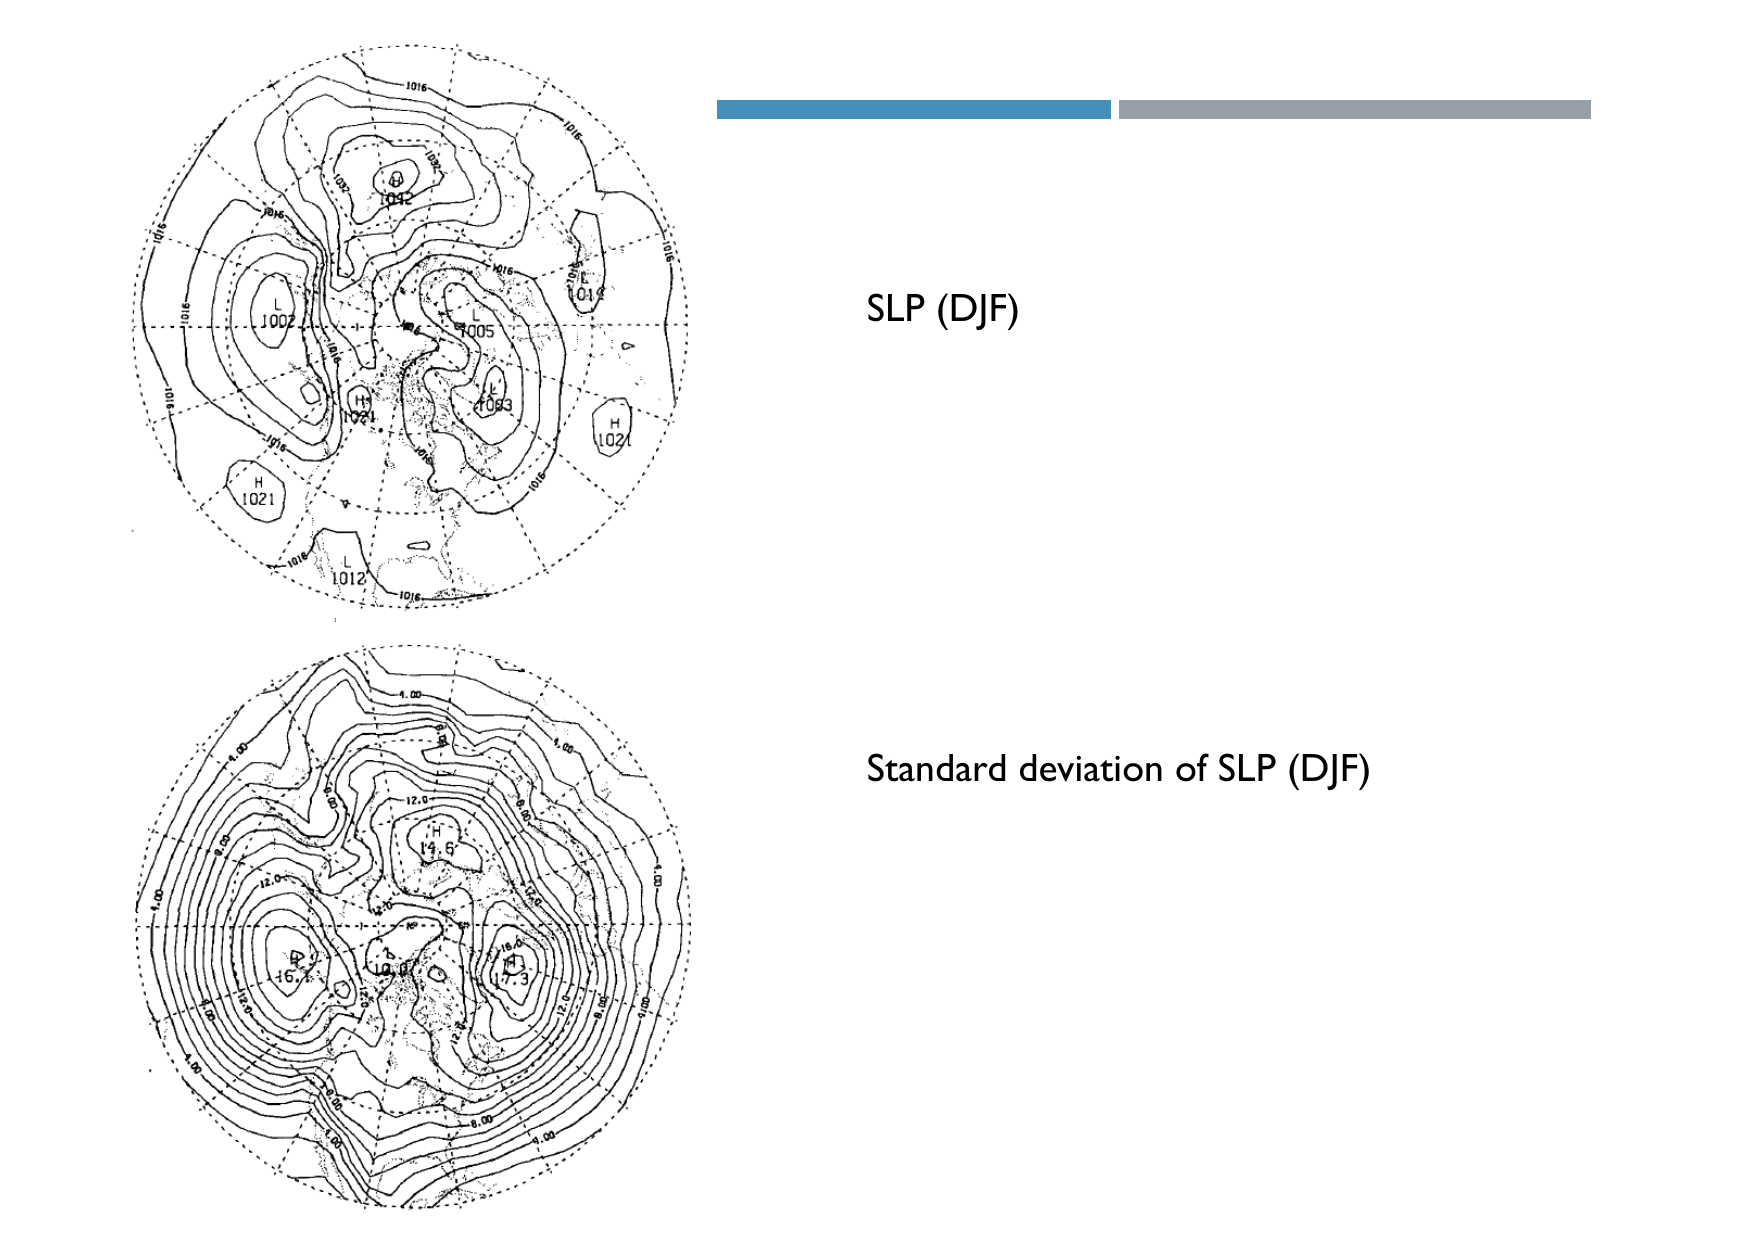
\includegraphics[width=0.85\textwidth]{images/ch06/p04_img01.png}
  \caption{Time-mean sea-level pressure (SLP) over the Northern Hemisphere
  for boreal winter (DJF).  Two dominant low-pressure centers are seen over
  the North Pacific (Aleutian Low) and the North Atlantic (Icelandic Low),
  while a massive surface high (Siberian High) dominates the Eurasian
  continent.  These zonally asymmetric features are the surface signature
  of the stationary wave pattern. \hisu{북반구 겨울 평균 해면 기압도.
  알류샨 저기압, 아이슬란드 저기압이 두 storm track의 종점이고, 시베리아
  고기압은 대륙 위 열적 고기압이다 — stationary wave의 지표 모습이다.}}
  \label{fig:ch06_nh_slp_djf}
\end{figure}

세 가지 특징을 강조하자.

\begin{enumerate}
  \item \textbf{Aleutian Low}와 \textbf{Icelandic Low}는 두 storm track
        (Pacific, Atlantic)의 \textit{사이클론 종착지}이다.  Baroclinic
        wave가 동쪽으로 전파하다 약화/소멸하면서 그 시간 평균 효과로
        지표 저기압이 고정된다.
  \item \textbf{Siberian High}는 차가운 대륙 위 \textit{radiative cooling}
        과 안정한 경계층 형성에 의한 열적 고기압이다.  대륙-해양 열
        contrast가 가장 큰 겨울에 가장 강하다.
  \item 이 SLP 패턴은 \textbf{시간 평균}이지만 그 안에는 (a) 진짜로 거의
        움직이지 않는 stationary 성분과 (b) 시간 평균이 우연히 비대칭으로
        나오는 transient 사이클론의 누적 효과가 \textit{둘 다} 포함되어
        있다.  이를 분리하는 것이 다음 항목의 목표이다.
\end{enumerate}

\begin{hisublock}
SLP만으로는 stationary wave와 transient의 기여를 분리할 수 없다.  알류샨
저기압의 강도가 ``전선이 자주 지나가서 평균이 낮은 것''인지 아니면 ``평균
순환 자체에 저기압이 고정되어 있는 것''인지 답하려면 \textit{시간 필터링}이
필요하다.  Blackmon et al.\ (1977)이 도입한 low-pass / band-pass 분리법이
바로 이 질문에 대한 정량적 답을 제공한다 (§1.2 참조).
\end{hisublock}

% --------------------------------------------------------------------------
\subsubsection{Time Filtering: Low-Pass, High-Pass, Band-Pass}

NH 겨울 순환에서 \textgr{stationary wave}와 \textgr{transient eddy}를
분리하는 핵심 도구는 \textgr{time filtering}이다.  Blackmon et al.\ (1977)이
표준화한 framework를 따라 세 가지 필터를 정의한다.

\begin{definition}[Low-pass, High-pass, Band-pass Filters]
임의의 시계열 $X(t)$를 주파수 $\omega$ 성분으로 Fourier 분해하여
$X(t) = \int \widehat{X}(\omega)e^{i\omega t}d\omega$로 표현할 때, 필터 $F$의
\textgr{response function} $R_F(\omega)$를 통해 필터링된 시계열을
\begin{equation}\label{eq:ch06_nh_filter_def}
  X^F(t) = \int R_F(\omega)\,\widehat{X}(\omega)\,e^{i\omega t}\,d\omega
\end{equation}
로 정의한다.  세 가지 표준 필터는 다음과 같다:
\begin{itemize}
  \item \textbf{Low-pass} $R_L(\omega)$: $|\omega| < \omega_c$에서 $\approx 1$,
        그 이상에서 $\approx 0$ (느린 변동만 통과).
  \item \textbf{High-pass} $R_H(\omega) = 1 - R_L(\omega)$ (빠른 변동만 통과).
  \item \textbf{Band-pass} $R_B(\omega) = R_{L_1}(\omega) - R_{L_2}(\omega)$,
        $\omega_{c,1} > \omega_{c,2}$ — 두 low-pass의 차로 정의된 특정 대역.
\end{itemize}
\end{definition}

\hisu{Low-pass = 느린 신호만 통과 (stationary, 30일 이상);  High-pass = 빠른
신호 (2일 이하의 mesoscale);  Band-pass = 그 사이 (synoptic 2--7일,
baroclinic wave가 사는 대역).}

\begin{proposition}[Equivalent Forms of the Band-pass Response]
$R_H \equiv 1 - R_L$로 정의하면, band-pass 응답함수는
\begin{equation}\label{eq:ch06_nh_filter_eq}
  R_B(\omega) = R_H(\omega) \cdot R_{L'}(\omega)
              = R_{L_1}(\omega) - R_{L_2}(\omega),
\end{equation}
두 가지 동등한 표현이 가능하다.  앞은 ``빠른 성분에 다시 느린 cutoff를
씌운 것''이고, 뒤는 ``두 cutoff를 가진 low-pass의 차''이다.
\end{proposition}

\begin{proof}
정의에 의해 $R_H = 1 - R_L$이므로
$R_B = R_H R_{L'} = (1 - R_L) R_{L'} = R_{L'} - R_L R_{L'}$.
$\omega_{c,2} < \omega_{c,1}$인 경우 product $R_L R_{L'} \approx R_{L_2}$로
근사되며 결과적으로 $R_B \approx R_{L'} - R_{L_2} = R_{L_1} - R_{L_2}$이다.
\end{proof}

\begin{figure}[ht]
  \centering
  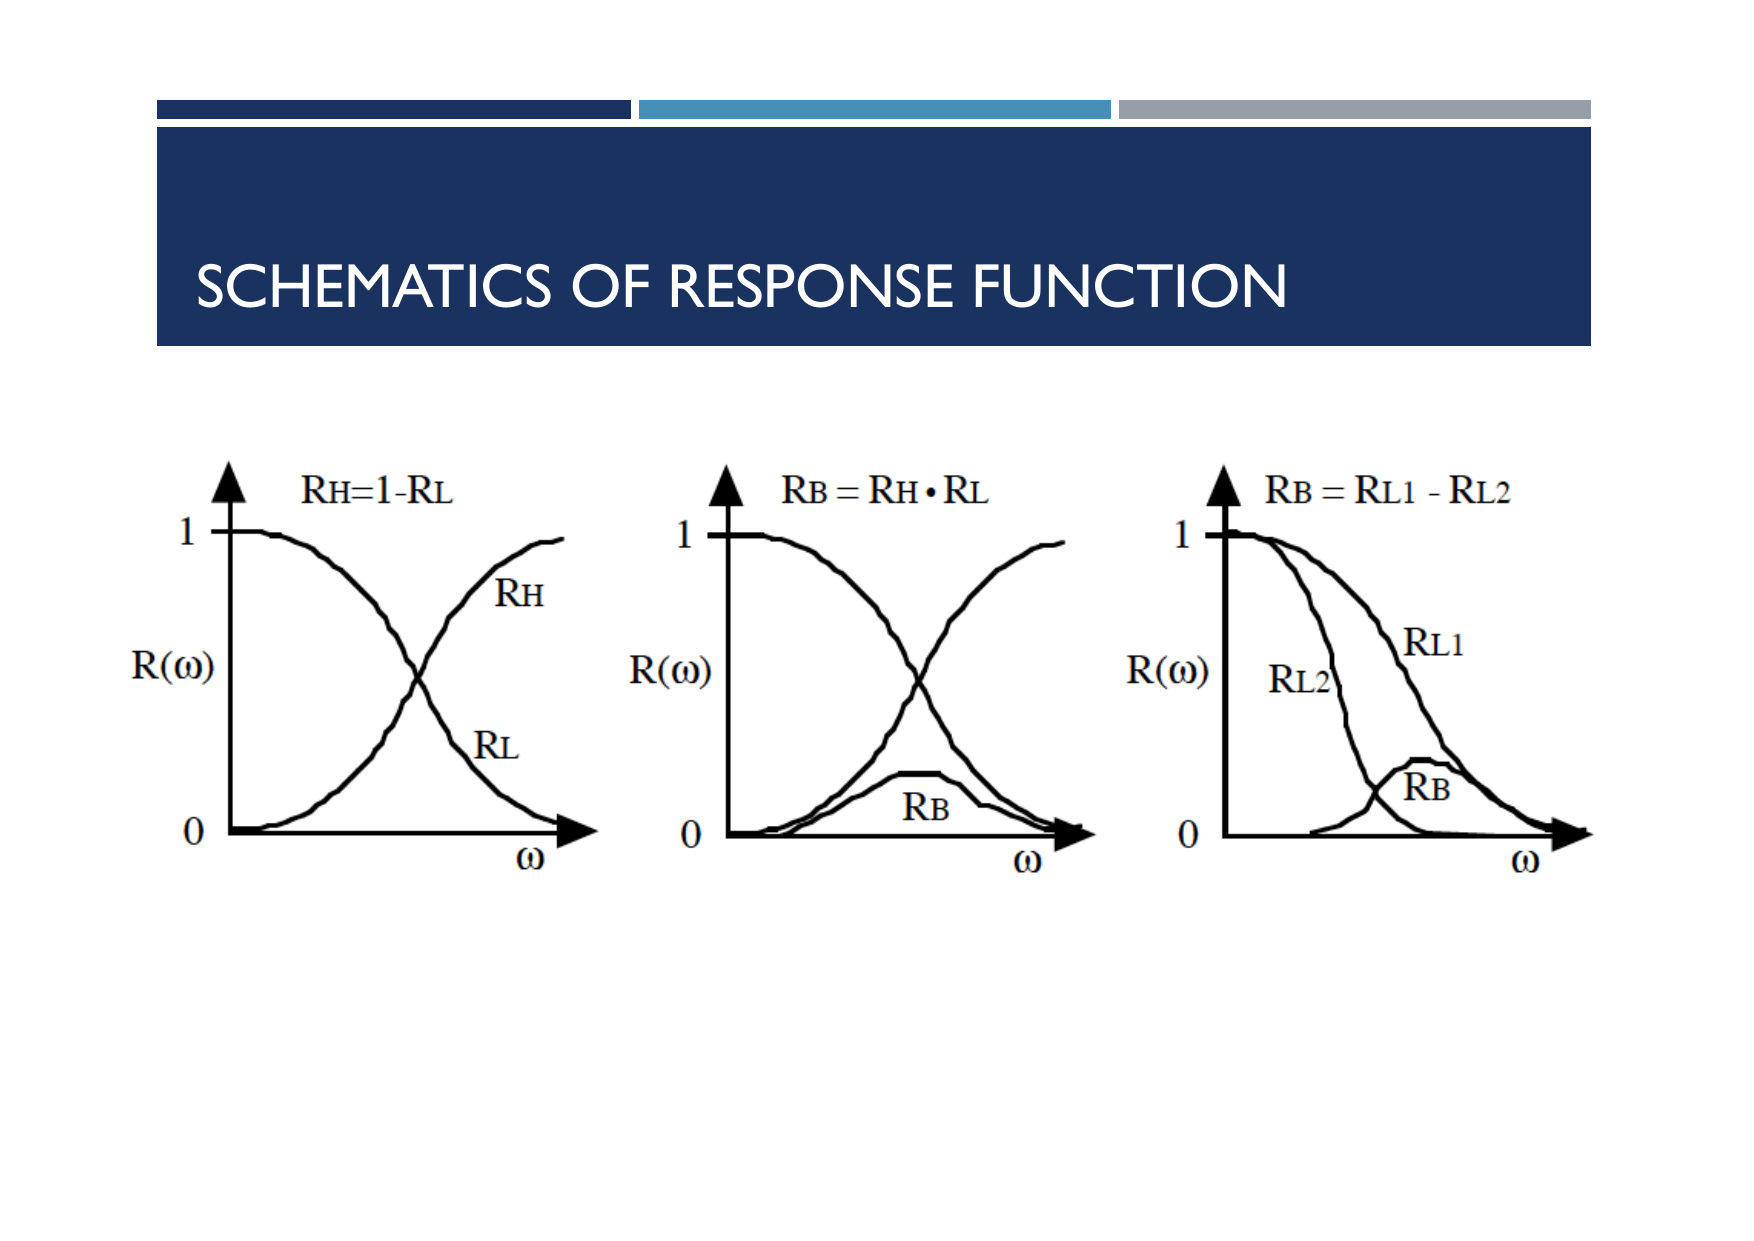
\includegraphics[width=0.5\textwidth]{images/ch06/p06_img01.png}
  \caption{Schematics of low-pass, high-pass, and band-pass response
  functions in the frequency domain.  The band-pass response, conventionally
  used to isolate synoptic-scale (2--7 day) baroclinic eddies, can be
  obtained either as the product $R_H \cdot R_L$ or as the difference of two
  low-pass filters with different cutoff frequencies. \hisu{응답함수 개념도.
  Band-pass는 (a) high-pass에 추가로 low-pass를 곱하거나, (b) 두 low-pass의
  차로 만들 수 있다 — Blackmon et al.\ (1977) 방식.}}
  \label{fig:ch06_nh_response}
\end{figure}

\begin{example}[Application to 50-yr GCM Pre-Industrial Run]
Blackmon et al.\ (1977)이 NCEP 관측 자료에 적용한 방식을 그대로 50년 GCM
pre-industrial control run의 일일 SLP에 적용하면 다음과 같은 분리가
가능하다.

\begin{itemize}
  \item \textbf{Low-pass} (cutoff $\sim 10$일): 30일 이상 시간 스케일의 변동.
        이것의 시간 평균이 \textit{stationary wave} 성분이다.
  \item \textbf{Band-pass} (2--7일): synoptic-scale baroclinic eddies.
        이 성분의 \textit{분산}이 storm track의 정의이다.
  \item \textbf{High-pass} ($<2$일): mesoscale 및 noise 성분.  일반적으로
        SLP에서는 작다.
\end{itemize}
\end{example}

\begin{figure}[ht]
  \centering
  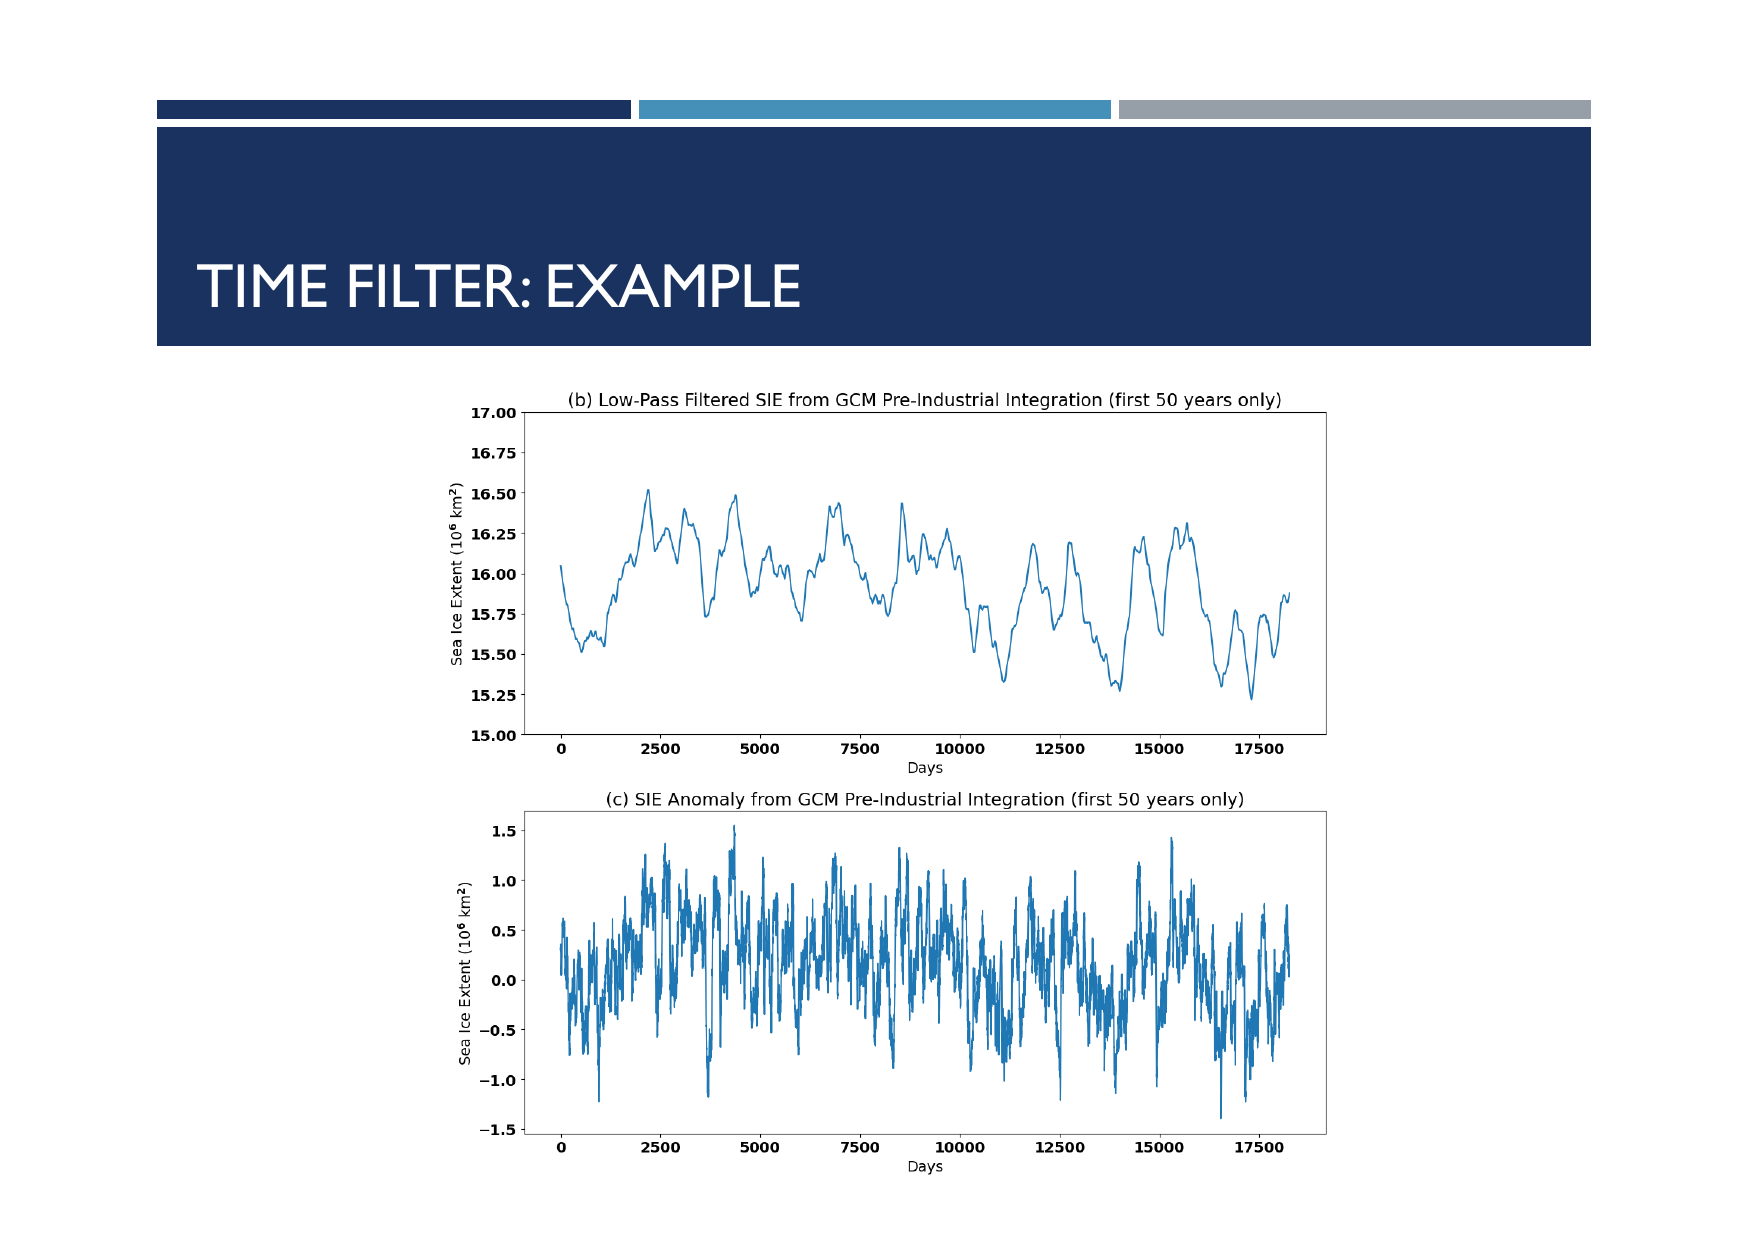
\includegraphics[width=0.85\textwidth]{images/ch06/p05_img01.png}
  \caption{Example application of a low-pass filter to a 50-yr
  pre-industrial GCM run.  The raw daily Sea Ice Extent (or analogous SLP)
  time series shows high-frequency noise, while the low-pass-filtered series
  reveals the slow climate-mode variability suitable for stationary-wave
  diagnosis. \hisu{시계열 필터링 예시 — 원시 일일자료에서 빠른 잡음을
  걸러내고 느린 기후 변동만 남기면 stationary 성분 분석이 가능해진다.}}
  \label{fig:ch06_nh_filter_example}
\end{figure}

\begin{remark}[Stationary vs.\ Transient Variance Decomposition]
표준편차 (분산의 제곱근) 지도를 low-pass와 band-pass에 대해 각각 그리면
물리적 의미가 명확하다.  Low-pass std는 ``느리게 변하는 기후 모드''의
지리적 분포 (PNA, NAO 등의 흔적)를 보여주고, band-pass std는
\textit{storm track} 그 자체이다.
\end{remark}

\begin{figure}[ht]
  \centering
  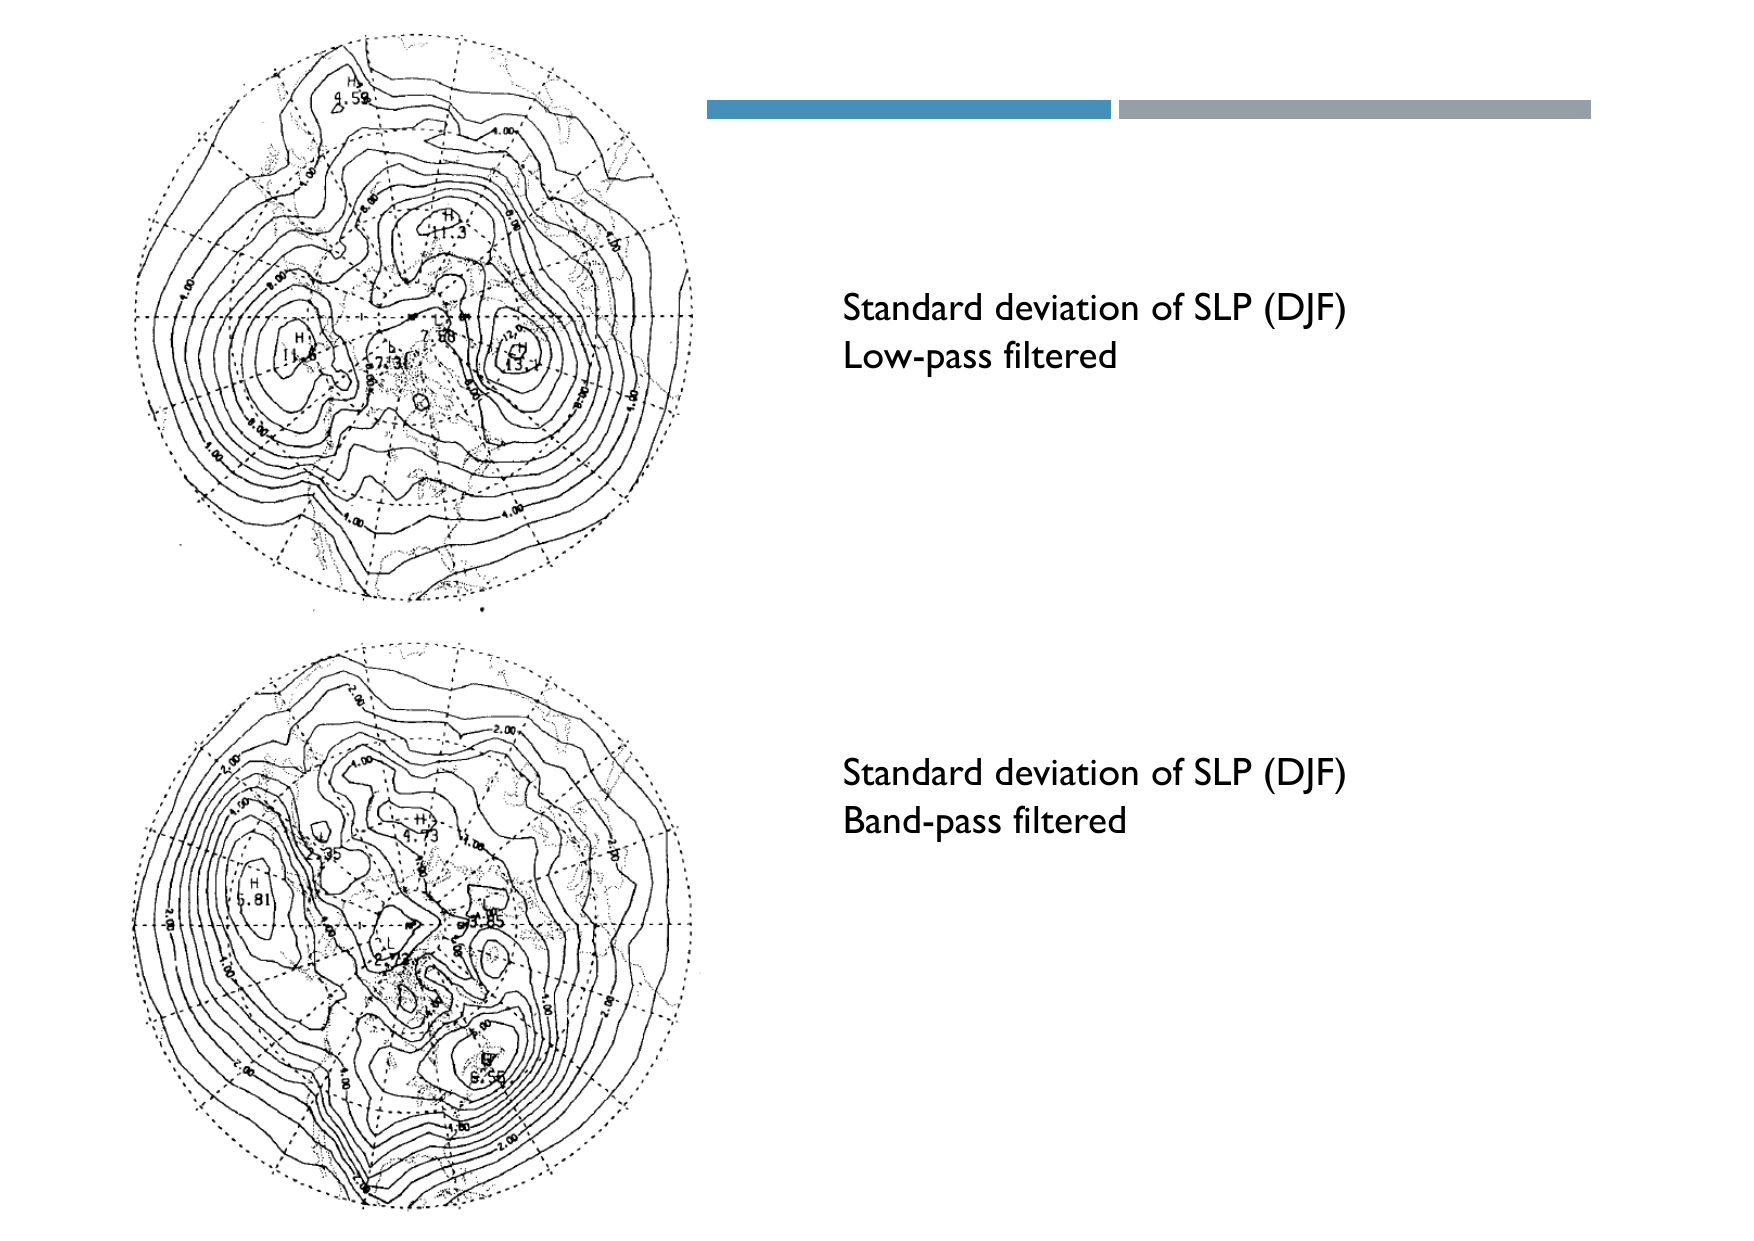
\includegraphics[width=0.85\textwidth]{images/ch06/p07_img01.png}
  \caption{Standard deviation of DJF SLP after low-pass filtering (left)
  and band-pass filtering (right).  Low-pass variance peaks over the
  high-latitude oceans and reflects slow climate modes, while band-pass
  variance peaks downstream of Japan and Newfoundland — these maxima
  \textit{define} the Pacific and Atlantic storm tracks. \hisu{Low-pass
  분산은 느린 기후 모드 (NAO 등)의 분포, band-pass 분산은 storm track 그
  자체의 정의 — 두 극대가 Pacific과 Atlantic storm track이다.}}
  \label{fig:ch06_nh_slp_std}
\end{figure}

\begin{hisublock}
Blackmon et al.\ (1977) Fig.~3과 비교하라.  원 논문에서는 500~hPa
geopotential height에 적용했지만, 본 figure는 SLP 버전이다.  결론은
동일하다: \textit{transient 분산은 시간 평균 등압선과 다른 위치에 극대를
가지며}, 이는 storm track이 평균 trough 위에 정확히 자리잡지 \textit{않음}
을 의미한다 (downstream-shifted, ageostrophic dynamics에 의해 — §1.4 참조).
\end{hisublock}

% --------------------------------------------------------------------------
\subsubsection{Eddy Flux Maps and Storm Tracks}

Transient eddy를 정량화하는 다음 단계는 \textit{flux}의 분포를 보는
것이다.  Eddy momentum flux $\overline{u'v'}$와 eddy heat flux
$\overline{v'T'}$는 storm track의 \textit{역학적} 특징을 정의한다.

\begin{definition}[Eddy Fluxes]
시간 평균을 $\overline{(\cdot)}$로, 그로부터의 편차 (high-pass 또는
band-pass) 성분을 $(\cdot)'$로 표기할 때,
\begin{equation}\label{eq:ch06_nh_eddy_def}
  u = \overline{u} + u',\qquad
  v = \overline{v} + v',\qquad
  T = \overline{T} + T'.
\end{equation}
\textgr{Eddy momentum flux}와 \textgr{eddy heat flux}는 각각
\begin{equation}\label{eq:ch06_nh_flux_def}
  \overline{u'v'}\quad(\text{poleward flux of zonal momentum}),\qquad
  \overline{v'T'}\quad(\text{poleward flux of heat})
\end{equation}
로 정의된다.  여기서 ``poleward''는 $v' > 0$일 때 양수가 됨을 뜻한다.
\end{definition}

\hisu{$\overline{u'v'}$는 ``동쪽 운동량을 북쪽으로 얼마나 운반하는가''
$\overline{v'T'}$는 ``열을 북쪽으로 얼마나 운반하는가''.  중위도에서 둘
다 양수이며, 이것이 baroclinic eddy의 본질이다.}

\begin{figure}[ht]
  \centering
  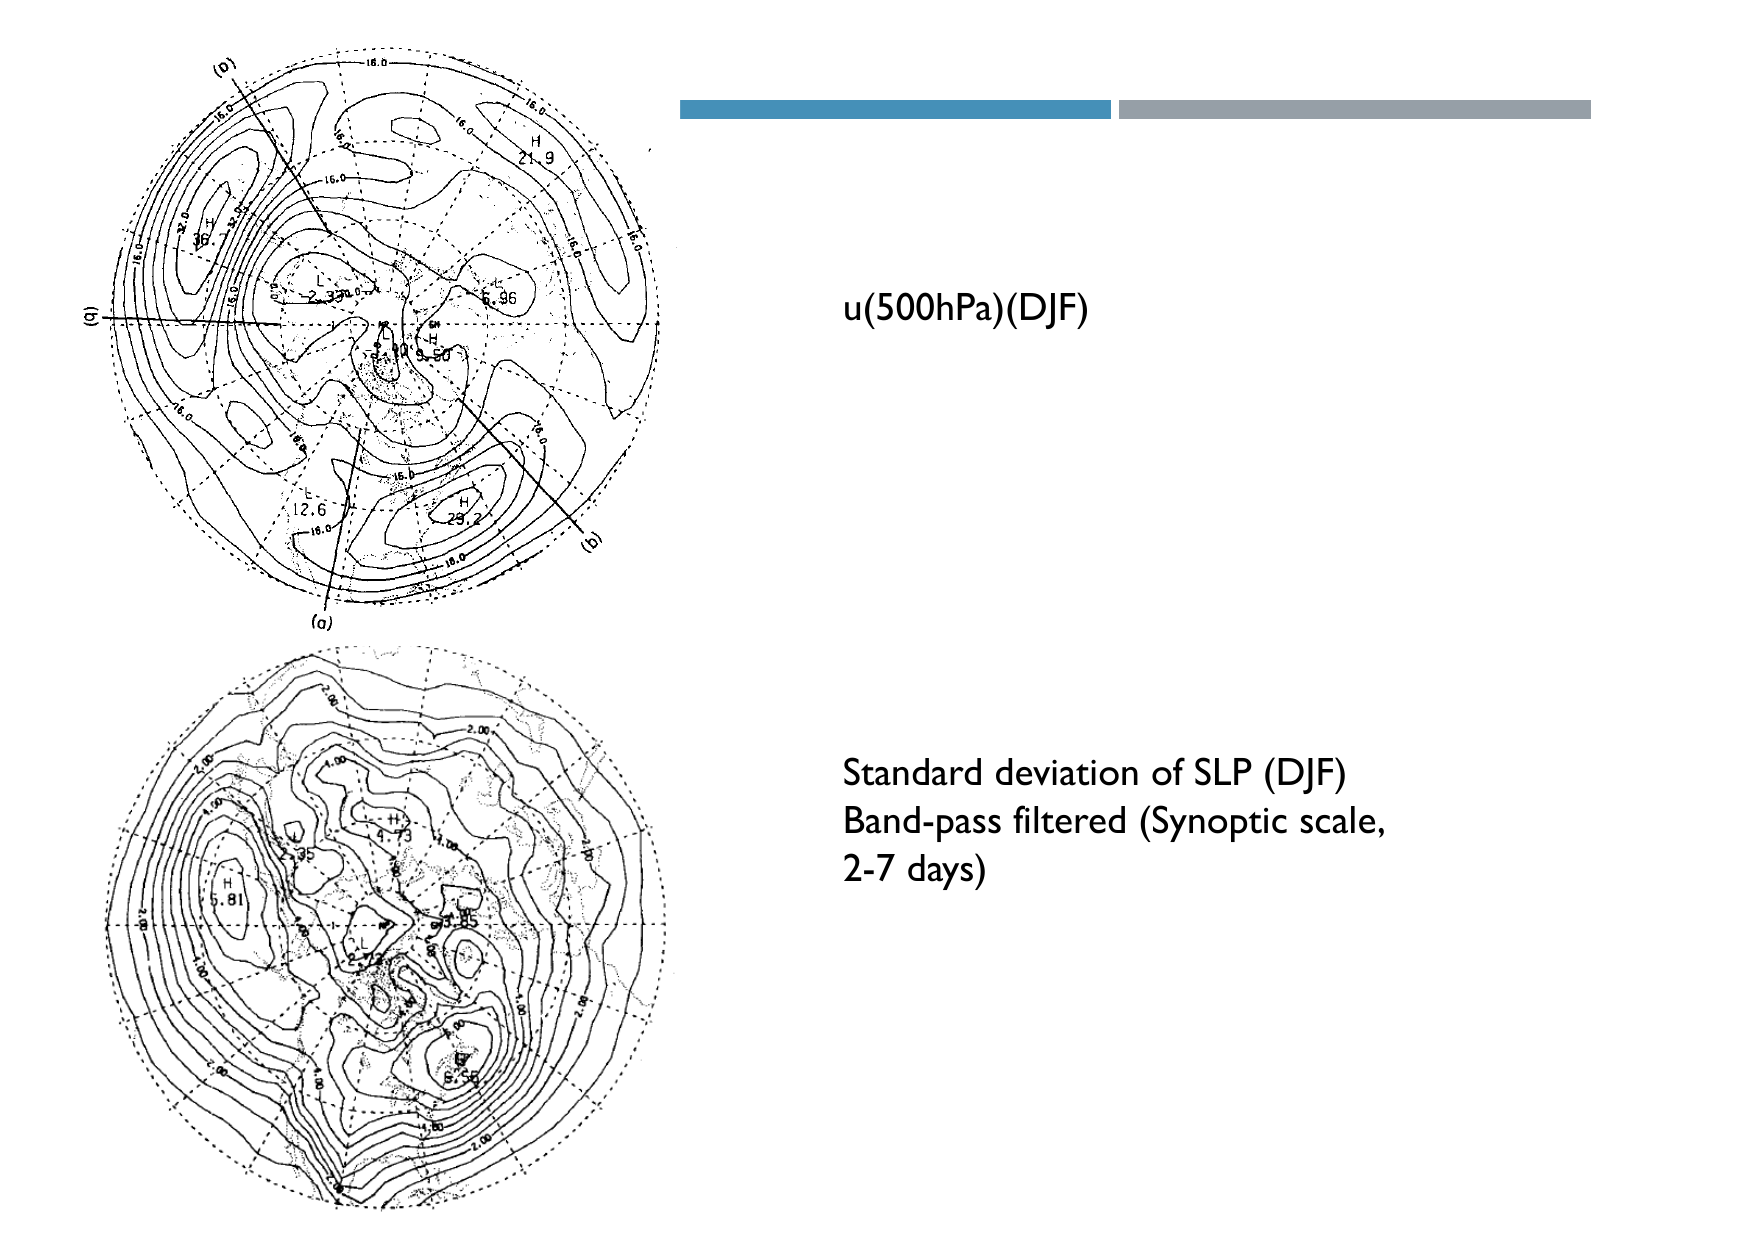
\includegraphics[width=0.85\textwidth]{images/ch06/p08_img01.png}
  \caption{Top: DJF time-mean zonal wind at 500~hPa, showing the two
  upper-tropospheric jet maxima over East Asia and the western Atlantic.
  Bottom: Standard deviation of band-pass (2--7 day) filtered $u$ at
  500~hPa, identifying the synoptic-scale storm tracks.  Note that the
  storm-track maxima lie \textit{downstream and slightly poleward} of the
  jet exit regions. \hisu{500~hPa zonal wind 평균과 synoptic band-pass 분산.
  Storm track 극대가 jet exit의 \textit{북동쪽}에 위치한다 — 이것이
  ageostrophic 메커니즘과 jet downstream maintenance를 시사한다.}}
  \label{fig:ch06_nh_u500_band}
\end{figure}

\begin{figure}[ht]
  \centering
  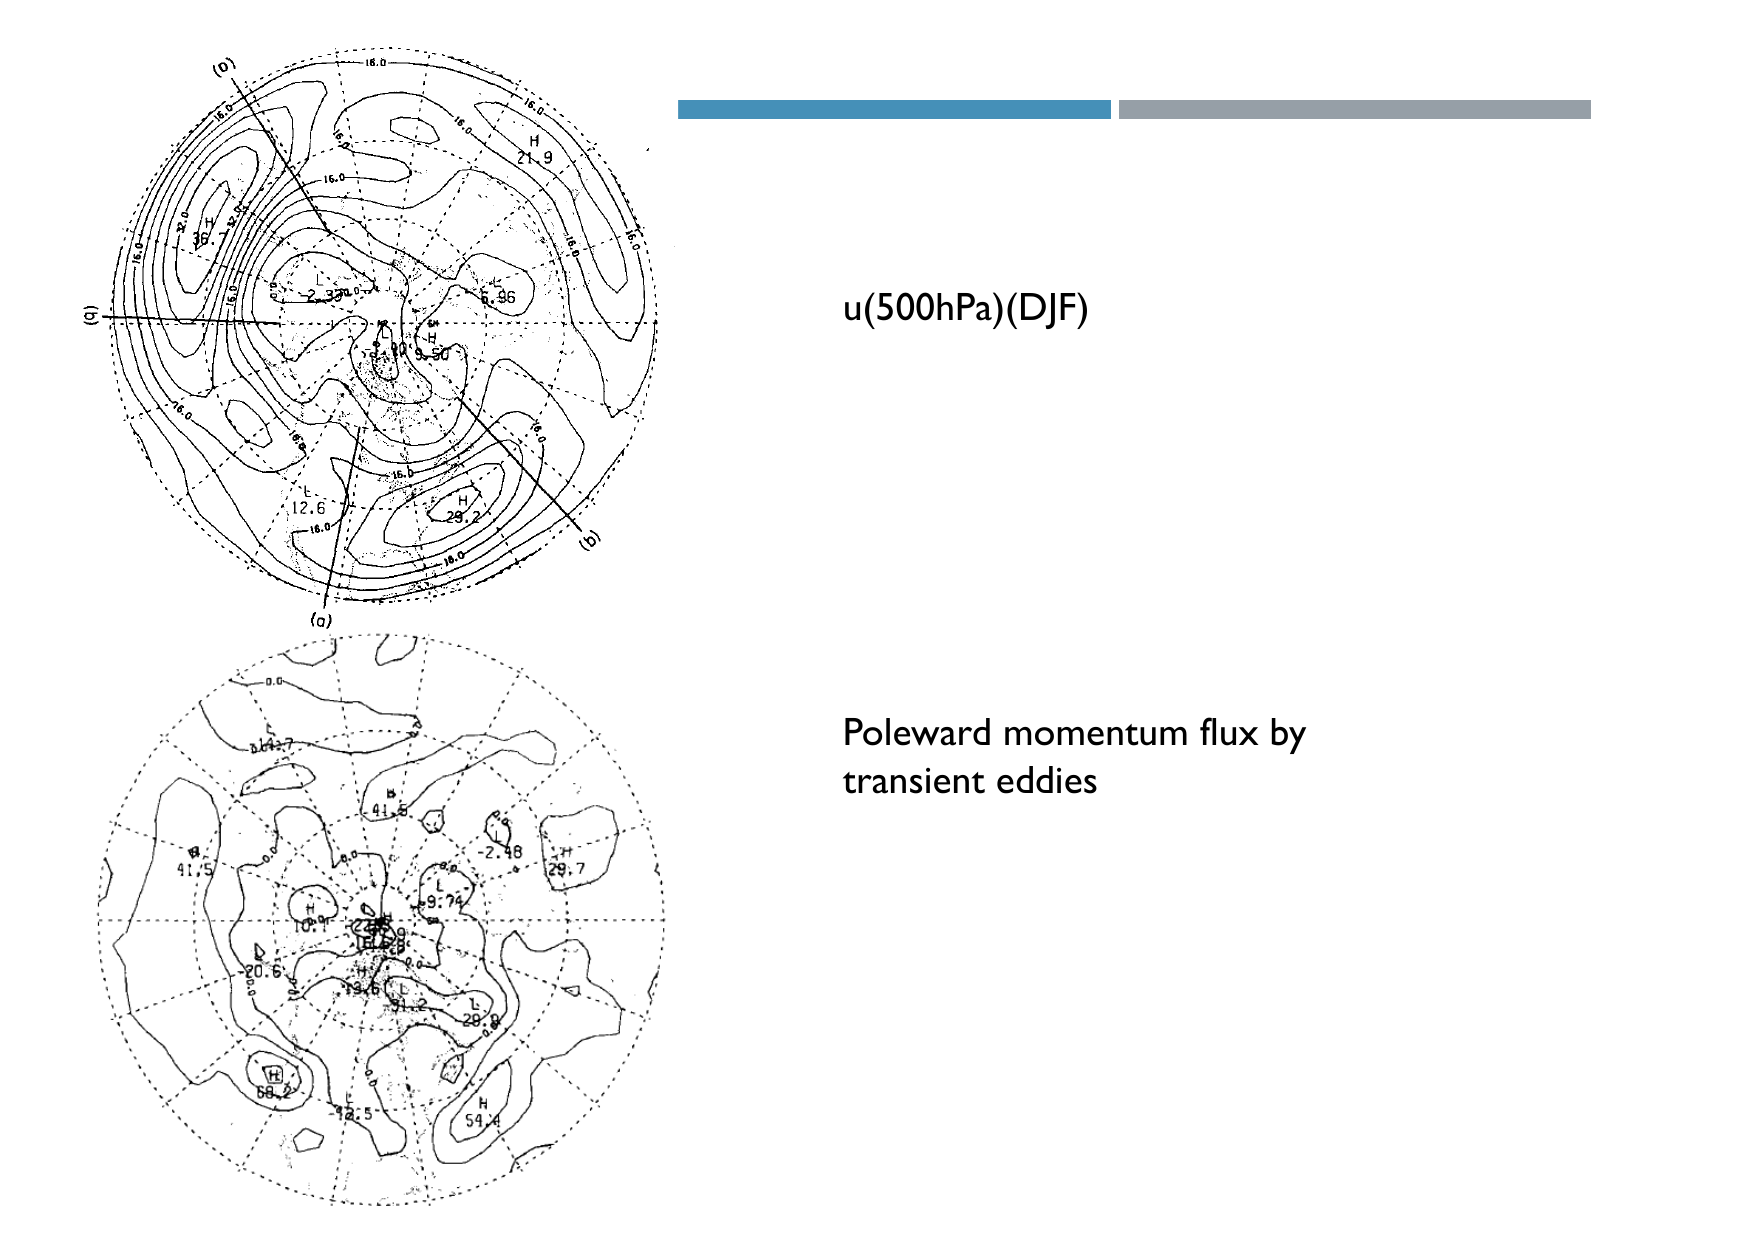
\includegraphics[width=0.85\textwidth]{images/ch06/p09_img01.png}
  \caption{Poleward eddy momentum flux $\overline{u'v'}$ at 300~hPa (top)
  and poleward eddy heat flux $\overline{v'T'}$ at 850~hPa (bottom) for DJF,
  using band-pass (2--7 day) filtered fields.  Both fluxes are predominantly
  \textit{positive} (poleward) in the storm-track regions, consistent with
  baroclinic conversion: eddies extract available potential energy from the
  mean equator-to-pole temperature gradient and transport heat poleward,
  while simultaneously fluxing westerly momentum into the jet core. \hisu{
  300~hPa의 $\overline{u'v'}$와 850~hPa의 $\overline{v'T'}$ 모두 storm track
  에서 양수 (북쪽 방향).  열은 북쪽으로, 운동량은 jet core 쪽으로 — 이것이
  baroclinic eddy가 평균 흐름을 \textit{유지}하는 메커니즘이다.}}
  \label{fig:ch06_nh_eddy_flux}
\end{figure}

\begin{remark}[Why the Eddy Fluxes Are Positive in Mid-latitudes]
중위도에서 $\overline{u'v'} > 0$인 이유는 baroclinic wave의 위상이
북동-남서 (SW--NE) 방향으로 기울어져 있기 때문이다.  trough 서쪽에서는
$u' > 0$이고 $v' > 0$ (남서풍 가속), 동쪽에서는 $u' < 0$이고 $v' < 0$.
둘 다 곱 $u'v' > 0$이 되어 시간 평균이 양수로 나온다.  $\overline{v'T'}$도
유사하게, 따뜻한 공기가 북쪽으로 (warm $v' > 0$), 찬 공기가 남쪽으로
($T' < 0$이면서 $v' < 0$) 이동하므로 둘 다 양수 곱이 된다.
\end{remark}

\begin{hisublock}
Blackmon et al.\ (1977) Fig.~6과 Lau (1979a) Figs.~2, 4가 이 figure의
원본이다.  특히 Lau (1979a)는 두 storm track의 \textit{vertical structure}
까지 다루며 baroclinic conversion $C(\overline{P}_M, P_T)$와
$C(P_T, K_T)$의 지리적 분포를 보여준다 — 이는 본 챕터 §2에서 다룬다.
관측 사실 한 가지: poleward heat flux 극대는 \textit{lower troposphere}
(850~hPa), poleward momentum flux 극대는 \textit{upper troposphere}
(300~hPa)에 있다.  이 vertical 분리가 §3의 stationary wave maintenance
논의에 핵심 단서이다.
\end{hisublock}

\begin{proposition}[Eddy Kinetic Energy and Heat Variance]
Band-pass 필터된 $u', v', T'$로부터 다음 두 진단량을 정의한다:
\begin{equation}\label{eq:ch06_nh_KT_def}
  K_T \;\equiv\; \tfrac{1}{2}\,\overline{(u'^2 + v'^2)},
\end{equation}
\begin{equation}\label{eq:ch06_nh_TT_def}
  \overline{T'^2}
  \;=\; \text{eddy temperature variance.}
\end{equation}
$K_T$는 \textgr{transient (eddy) kinetic energy}이며, $\overline{T'^2}$는
storm track의 thermal intensity를 측정한다.
\end{proposition}

\hisu{$K_T = \tfrac{1}{2}\overline{(u'^2+v'^2)}$는 ``요란의 운동에너지 밀도'',
$\overline{T'^2}$는 ``요란의 온도 분산'' — 강의 슬라이드의 표기 $\tfrac{1}{2}
\overline{(u'^2 v'^2)}$는 명백한 typo이며 본 책에서는 표준 형식
\eqref{eq:ch06_nh_KT_def}을 사용한다.}

\begin{remark}[Heat Flux and Baroclinicity]
$\overline{v'T'} > 0$ (북쪽으로 열 운반)이 발생하는 \textit{물리적 조건}은
$\partial \overline{T}/\partial y < 0$ — 즉 평균 온도가 북쪽으로 갈수록
낮아지는 \textit{baroclinic} mean state이다.  이 mean gradient를 ``소비''
하면서 eddy가 자라며, 이때 eddy potential energy $P_T$가 생성된다.
$\overline{v'T'}$ 지도와 평균 등온선 지도를 겹쳐 그리면 두 storm track이
가장 강한 baroclinic 영역과 정확히 일치함을 확인할 수 있다.
\end{remark}

% --------------------------------------------------------------------------
\subsubsection{Jet Stream Geometry and the Ageostrophic Wind}

Jet stream은 \textit{지역적으로} 강한 zonal wind maximum이다.  중요한
질문: 왜 jet entrance에서 \textit{입자가 가속}되고 exit에서 \textit{감속}
되는가?  이 비대칭은 \textgr{ageostrophic wind} $\mathbf{v}_a$에 의해
조정된다.

\begin{definition}[Ageostrophic Wind]
전체 수평 바람을 geostrophic 성분과 그 편차로 분해하면
\begin{equation}\label{eq:ch06_nh_ageo_def}
  \mathbf{v} = \mathbf{v}_g + \mathbf{v}_a,\qquad
  \mathbf{v}_g \equiv \frac{1}{f}\,\hat{\mathbf{k}}\times\nabla\Phi,
\end{equation}
여기서 $\Phi$는 geopotential, $f$는 Coriolis parameter이다.
$\mathbf{v}_a$를 \textgr{ageostrophic wind}라 부른다.
\end{definition}

\hisu{Geostrophic wind: 등압선에 평행 (PGF와 CoF가 정확히 균형).
Ageostrophic wind: 그 균형이 살짝 깨졌을 때의 작은 편차 — 그러나 이
작은 편차가 jet entrance/exit의 입자 가속·감속을 \textit{전부} 만든다.}

\begin{figure}[ht]
  \centering
  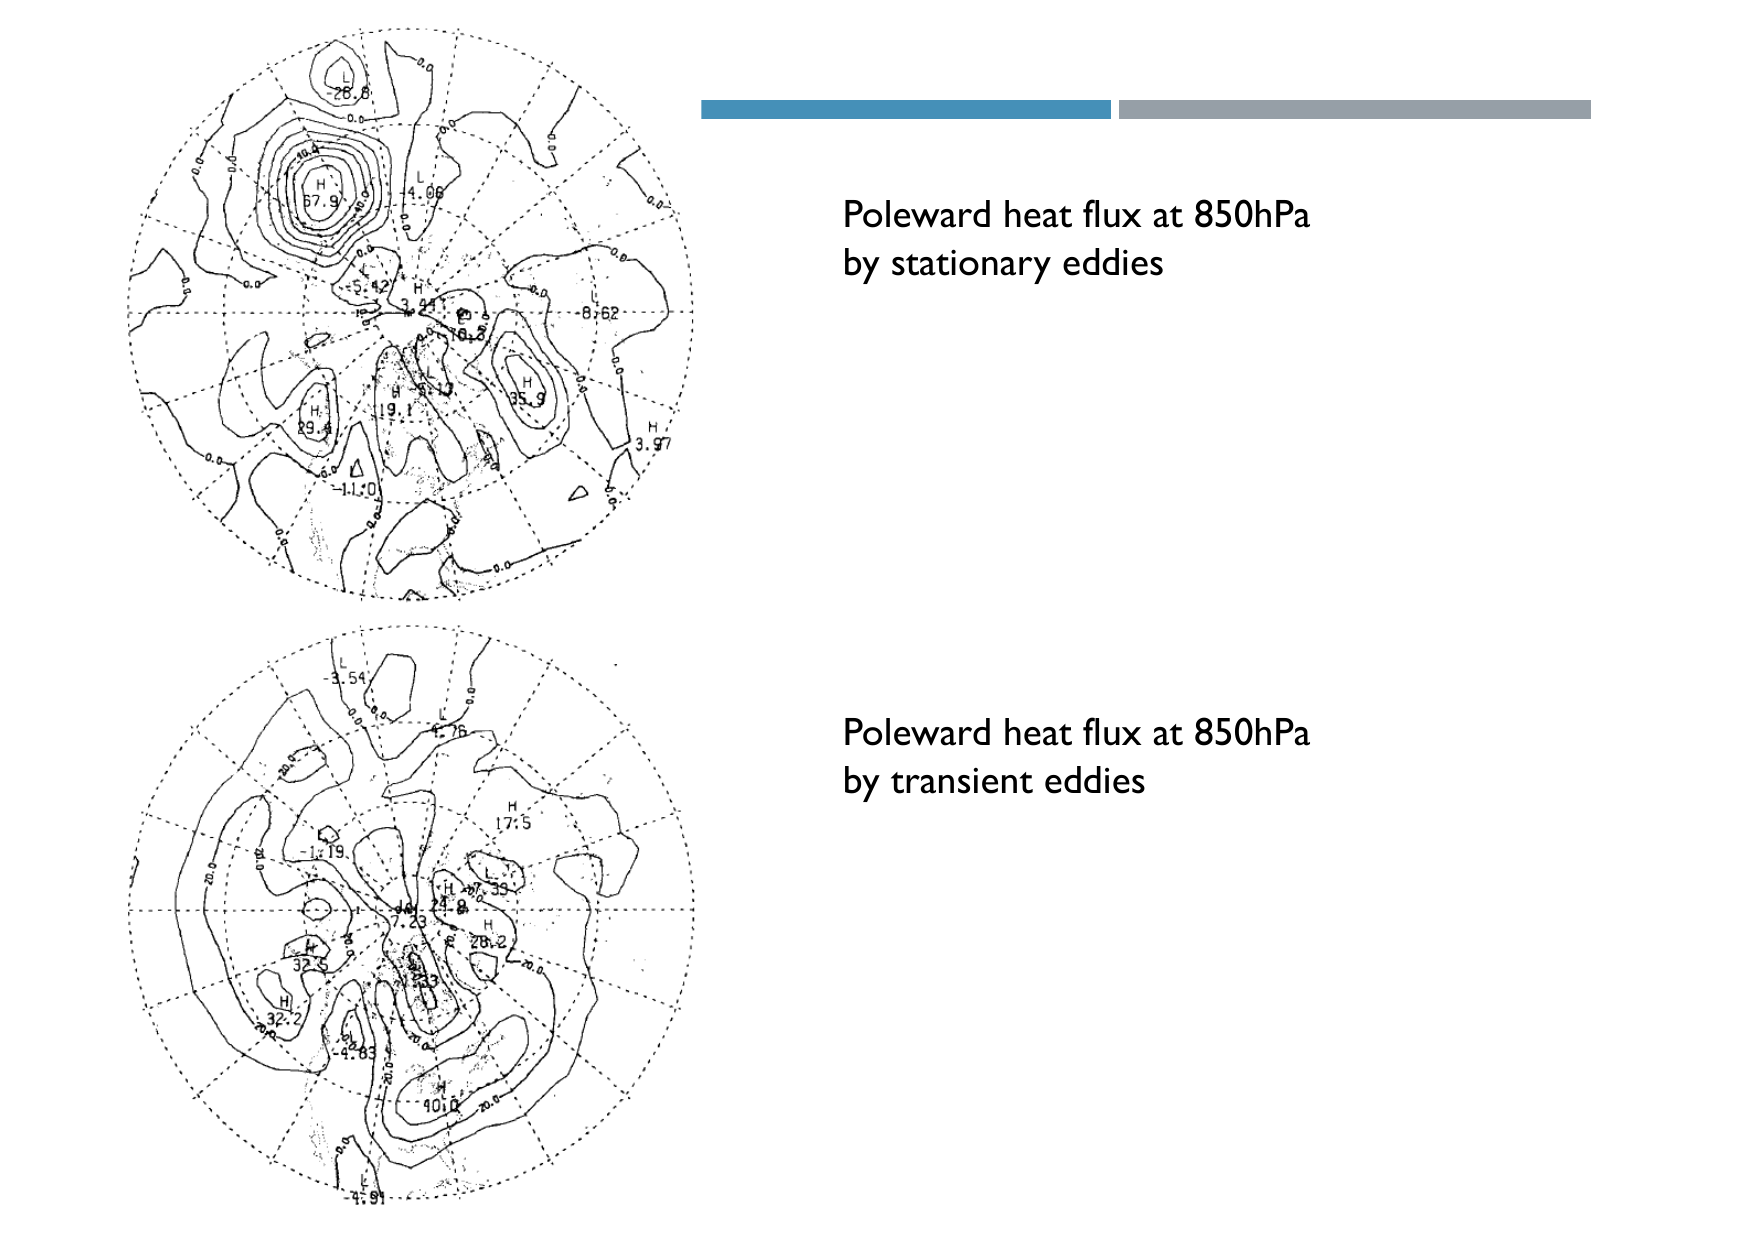
\includegraphics[width=0.85\textwidth]{images/ch06/p10_img01.png}
  \caption{Schematic of the ageostrophic wind associated with a localized
  jet streak.  At the \textbf{jet entrance}, parcels accelerate as they
  enter higher-wind region; the pressure-gradient force (PGF, poleward)
  exceeds the Coriolis force (CoF, equatorward), inducing a poleward
  ageostrophic component $v_a > 0$ in the entrance region.  At the
  \textbf{jet exit}, the situation reverses, producing $v_a < 0$
  (equatorward). \hisu{Jet entrance: PGF가 CoF보다 커서 입자가 \textit{북쪽으로}
  벗어남 ($v_a > 0$).  Exit: 반대로 \textit{남쪽으로} ($v_a < 0$).  이
  비대칭이 jet streak 주변의 4-cell vertical motion pattern을 만든다.}}
  \label{fig:ch06_nh_ageo_schem}
\end{figure}

물리적 직관은 다음과 같다.  Jet entrance에서 공기 입자는 약한 wind 지역에서
강한 wind 지역으로 진입한다.  진입 직전 입자는 약한 등압면 경사에 맞춰 약한
PGF와 약한 CoF가 균형을 이루는 상태이다.  그러나 강한 jet core 쪽으로 다가
가면 등압면 경사가 급해지므로 \textit{PGF는 즉시 강해지지만} (지위 분포에 의해
결정), Coriolis 힘은 입자의 \textit{실제 속도}에 비례하므로 입자가 아직 충분히
가속되지 않은 상태에서 약하게 남는다.  따라서 PGF $>$ CoF가 되어 입자는
PGF 방향으로 (북반구에서는 일반적으로 \textit{북쪽}으로) 미세하게 가속되는
ageostrophic 성분 $v_a > 0$을 갖는다.  Exit에서는 반대로 입자가 속도를 잃기
전에 CoF가 여전히 크므로 PGF $<$ CoF, 따라서 $v_a < 0$ (남쪽).

\begin{figure}[ht]
  \centering
  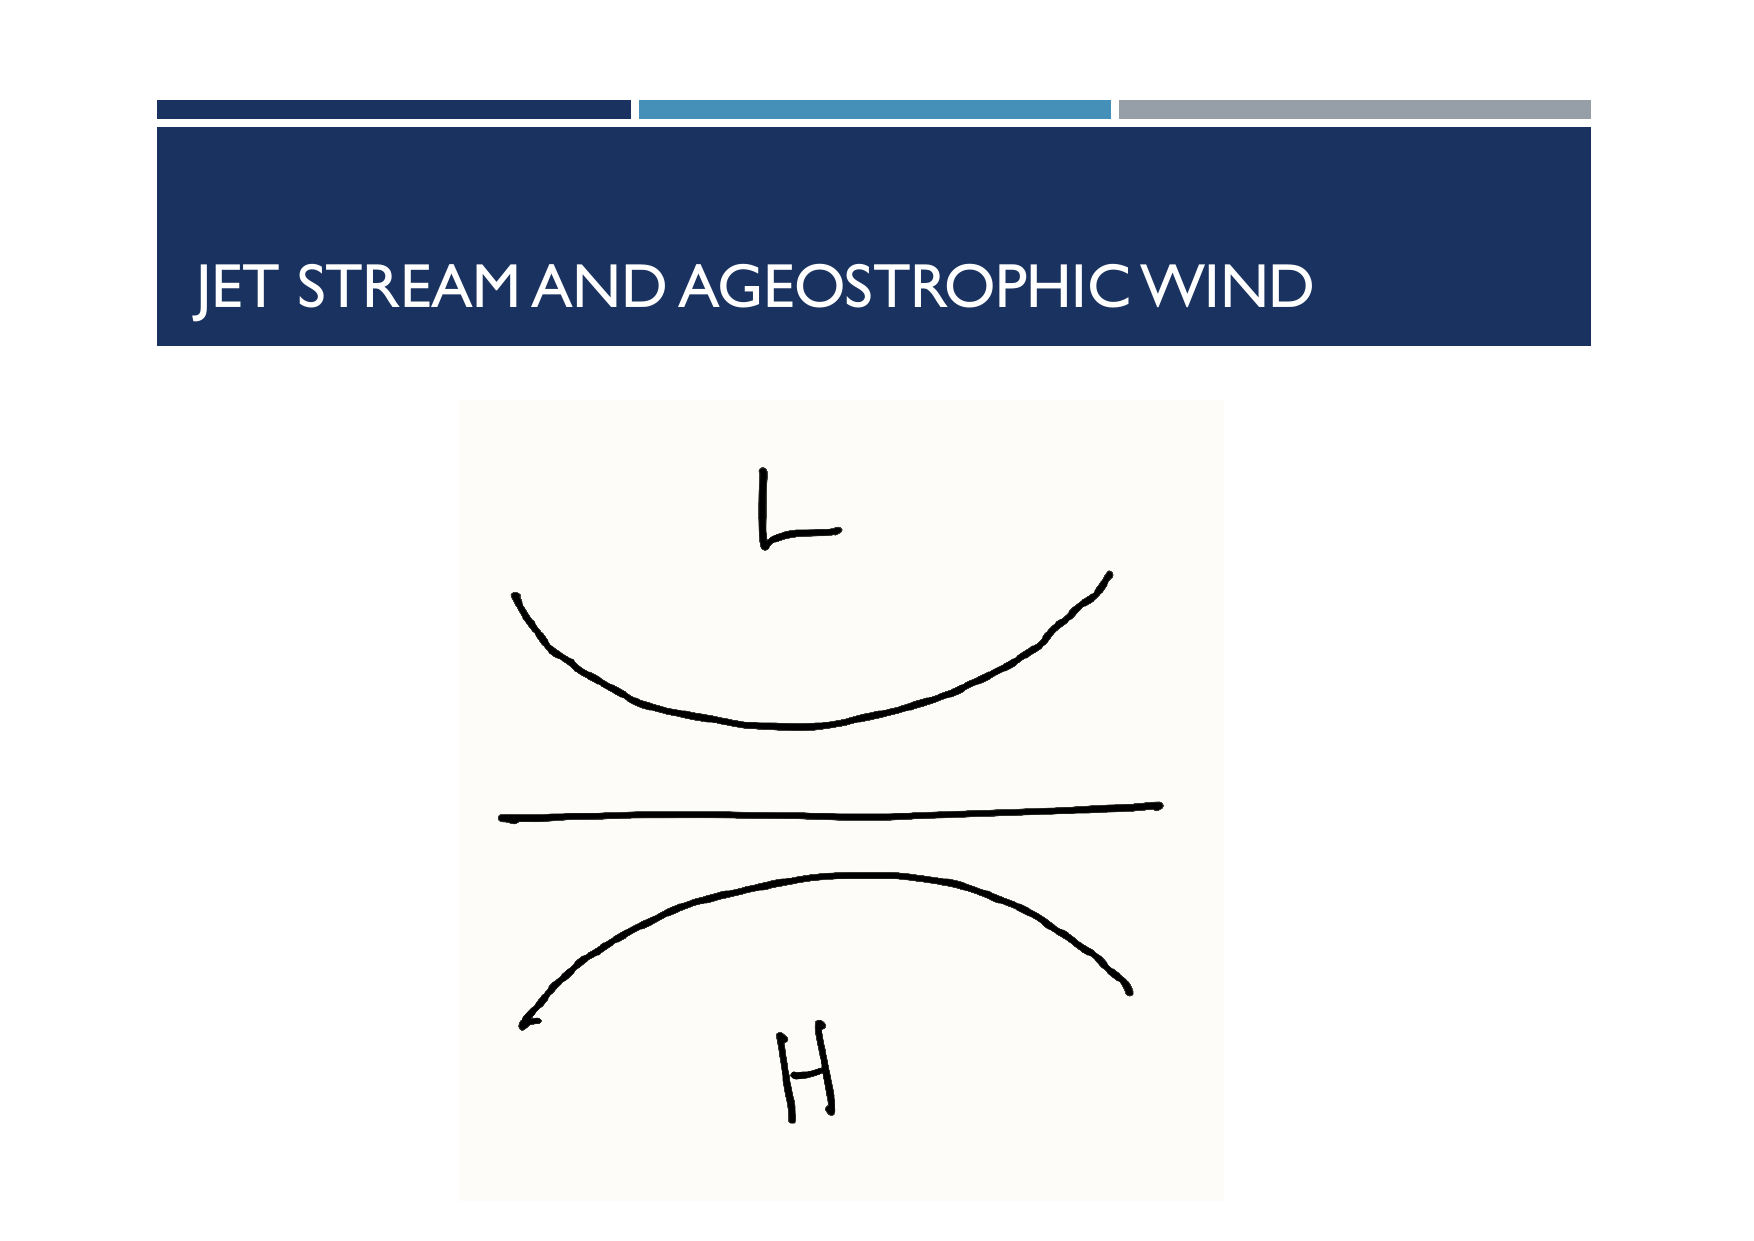
\includegraphics[width=0.85\textwidth]{images/ch06/p12_img01.png}
  \caption{Force balance in jet entrance versus jet exit regions.
  \textbf{Entrance:} PGF (poleward) $>$ CoF (equatorward), so the net force
  is poleward, producing $v_a > 0$ and parcel acceleration along the jet.
  \textbf{Exit:} PGF $<$ CoF, net force is equatorward, producing $v_a < 0$
  and parcel deceleration.  The associated ageostrophic divergence/convergence
  pattern drives vertical motion: ascent at the entrance equatorward side
  and exit poleward side, descent at the entrance poleward side and exit
  equatorward side. \hisu{Entrance에서 PGF $>$ CoF (북향 net force), exit에서
  PGF $<$ CoF (남향 net force).  이 두 ageostrophic 영역이 jet streak 주변
  대각선 4-cell rising/sinking 패턴을 만들고, 이것이 storm track 강화에 기여
  한다.}}
  \label{fig:ch06_nh_jet_force}
\end{figure}

\begin{hisublock}
이 그림의 4-cell 패턴은 단순한 도식이 아니다.  Entrance equatorward와 exit
poleward에서의 상승 (ascent)은 baroclinic instability에 필요한 vertical
motion을 \textit{이미 mean state로부터 공급}한다.  따라서 storm track이
``jet exit의 북동쪽''에 자리잡는 관측 사실 (Fig.~\ref{fig:ch06_nh_u500_band}
참조)이 자연스럽게 설명된다 — Pacific storm track은 일본 동쪽 (Pacific jet
exit), Atlantic storm track은 뉴펀들랜드 동쪽 (Atlantic jet exit) 부근에서
극대를 가진다.
\end{hisublock}

% --------------------------------------------------------------------------
\subsubsection{Q-G Momentum Equation Interpretation}

위에서 그림으로 설명한 ageostrophic wind와 jet entrance/exit dynamics를
이제 \textgr{quasi-geostrophic (Q-G) momentum equation}으로 정량화하자.
Beta-plane 근사에서 출발한다.

\begin{definition}[Quasi-Geostrophic Momentum Equations]
$f = f_0 + \beta y$로 전개하고 $|\mathbf{v}_a| \ll |\mathbf{v}_g|$의 scaling
하에서, $x$- 및 $y$-momentum 방정식의 \textgr{Q-G approximation}은
\begin{align}
  \frac{d_g u_g}{dt} - f_0 v_a - \beta y\,v_g &= 0, \label{eq:ch06_nh_qg_u}\\
  \frac{d_g v_g}{dt} + f_0 u_a + \beta y\,u_g &= 0, \label{eq:ch06_nh_qg_v}
\end{align}
여기서 $d_g/dt \equiv \partial/\partial t + \mathbf{v}_g\cdot\nabla$는
geostrophic material derivative이다.
\end{definition}

\hisu{Q-G 운동방정식: 평균 흐름은 geostrophic, 가속·감속은 ageostrophic
$\mathbf{v}_a$가 담당.  $\beta y$ 항은 $f$의 위도 변화 효과.}

\begin{proposition}[Local Acceleration in Jet Entrance/Exit]
시간 평균이 아닌 \textit{국지적} 시간 변화율을 고려할 때,
\eqref{eq:ch06_nh_qg_u}은
\begin{equation}\label{eq:ch06_nh_qg_simple}
  \frac{\partial u_g}{\partial t} \approx f_0\, v_a
\end{equation}
로 단순화된다 (이류 항과 $\beta y v_g$ 항이 다른 항들에 비해 작은 영역에서).
\end{proposition}

\begin{proof}
\eqref{eq:ch06_nh_qg_u}을 전개하면
$\partial u_g/\partial t + \mathbf{v}_g\cdot\nabla u_g - f_0 v_a - \beta y v_g = 0$.
Jet entrance 부근에서는 본질적으로 시간 변화 ($\partial u_g/\partial t > 0$,
즉 \textit{가속})와 ageostrophic 항이 가장 크고 나머지는 부차적이므로,
\eqref{eq:ch06_nh_qg_simple}이 leading-order balance가 된다.
\end{proof}

\begin{example}[Magnitude of $v_a$ at 30°N]
$f_0 = 2\Omega\sin 30° = 2 \times 7.292\times 10^{-5} \times 0.5
= 7.292 \times 10^{-5}~\mathrm{s}^{-1}$로 평가하자.  Jet entrance에서 입자가
하루 ($\sim 86400$~s) 동안 $\Delta u_g = 10~\mathrm{m\,s^{-1}}$ 정도 가속된다고
하면,
\begin{align*}
  \frac{\partial u_g}{\partial t}
    &\approx \frac{10~\mathrm{m\,s^{-1}}}{86400~\mathrm{s}}
     \approx 1.16\times 10^{-4}~\mathrm{m\,s^{-2}}.
\end{align*}
\eqref{eq:ch06_nh_qg_simple}에서
\begin{equation}\label{eq:ch06_nh_va_estimate}
  v_a \approx \frac{1}{f_0}\frac{\partial u_g}{\partial t}
    \approx \frac{1.16\times 10^{-4}}{7.292\times 10^{-5}}
    \approx 1.6~\mathrm{m\,s^{-1}}.
\end{equation}
\end{example}

\hisu{$v_a \sim 1$--$2~\mathrm{m\,s^{-1}}$ — 전체 wind $\sim 30~\mathrm{m\,s^{-1}}$의
5\% 정도.  작지만 무시할 수 없는 양으로, 이것이 jet entrance/exit의 가속을
유지한다.}

\begin{remark}[Connection to Vertical Motion]
\eqref{eq:ch06_nh_qg_v}로부터 유사하게
$\partial v_g/\partial t \approx -f_0 u_a$를 얻는다.  Continuity equation
$\nabla\cdot\mathbf{v}_a + \partial\omega/\partial p = 0$과 결합하면 (mass
continuity, ageostrophic이 divergence를 담당),
\begin{equation}\label{eq:ch06_nh_omega_div}
  \frac{\partial \omega}{\partial p}
    = -\nabla\cdot\mathbf{v}_a
    = -\left(\frac{\partial u_a}{\partial x} + \frac{\partial v_a}{\partial y}\right).
\end{equation}
즉 ageostrophic wind의 divergence가 vertical motion $\omega$를 직접 만든다.
Jet entrance equatorward쪽에서 $v_a > 0$ (북쪽) 성분의 발산은 상층에서
divergence, 따라서 $\partial\omega/\partial p < 0$ — 상승 운동을 의미한다.
\end{remark}

\begin{example}[Scale Analysis: Why Q-G Approximation Holds]
중위도 30°N에서 typical synoptic scale을 $L \sim 10^6$~m, 풍속을 $U \sim
30~\mathrm{m\,s^{-1}}$로 잡으면 \textgr{Rossby number}는
\begin{equation}\label{eq:ch06_nh_rossby}
  \mathrm{Ro} \;\equiv\; \frac{U}{f_0 L}
  \;\approx\; \frac{30}{7.292\times 10^{-5} \times 10^6}
  \;\approx\; 0.41.
\end{equation}
$\mathrm{Ro} \ll 1$이라는 strict한 의미에서 매우 작지는 않지만 ($\sim 0.4$),
\eqref{eq:ch06_nh_va_estimate}에서 본 $|v_a|/|v_g| \sim 1.5/30 \approx 0.05
\sim \mathrm{Ro}^{1/2}$ 정도이며, Q-G 근사의 leading-order balance가
중위도 jet 부근에서 정량적으로 합리적임을 정당화한다.
\end{example}

\hisu{Rossby number $\sim 0.4$가 ``크지도 작지도 않은'' 값이지만, Q-G가
실제로 매우 잘 작동하는 것은 ageostrophic 성분이 추가로 작아서이다.
중위도 synoptic dynamics의 ``축복''.}

\begin{remark}[Beta Term and Sverdrup-Like Balance]
\eqref{eq:ch06_nh_qg_u}의 $\beta y v_g$ 항을 잠시 leading order에 포함시키면,
\textit{시간 평균} ($\partial u_g/\partial t = 0$) 상태에서
\begin{equation}\label{eq:ch06_nh_meanbalance}
  f_0 \overline{v}_a \;=\; -\,\beta y\,\overline{v}_g
  + \overline{\mathbf{v}_g\cdot\nabla u_g},
\end{equation}
즉 시간 평균된 ageostrophic meridional wind는 (i) $\beta$ 효과와 (ii) 흐름의
운동량 advection으로부터 결정된다.  이것이 §3에서 다룰 \textit{stationary
wave 유지 방정식}의 출발점이며, Held (1983)가 mountain-forced wave에서
체계적으로 다룬 framework이다.
\end{remark}

\begin{hisublock}
이 절의 결론을 종합하면:
\begin{enumerate}
  \item DJF SLP의 비대칭 패턴 (Aleutian Low, Siberian High, Icelandic Low)은
        stationary wave + transient eddy 누적의 결과이다.
  \item 시간 필터링 (Blackmon et al.\ 1977 방식, 식
        \eqref{eq:ch06_nh_filter_def}, \eqref{eq:ch06_nh_filter_eq})으로
        둘을 정량적으로 분리할 수 있다.
  \item Band-pass 분산의 극대는 \textit{storm track}을 정의하며 (Pacific,
        Atlantic), 그 위치는 jet exit의 북동쪽이다 (Fig.~\ref{fig:ch06_nh_u500_band}).
  \item Eddy fluxes $\overline{u'v'}, \overline{v'T'}$는 storm track에서
        양수 (poleward); 열은 850~hPa에서, 운동량은 300~hPa에서 극대.
  \item Jet streak 주변의 ageostrophic wind ($v_a \sim 1$--$2~\mathrm{m\,s^{-1}}$)
        가 Q-G momentum eq.\ \eqref{eq:ch06_nh_qg_simple}을 통해 jet
        entrance/exit의 가속·감속을 책임지고, 동시에
        \eqref{eq:ch06_nh_omega_div}을 통해 4-cell vertical motion을 만든다.
\end{enumerate}

\medskip
\textbf{다음 절(§2)로의 연결}: storm track에 살고 있는 transient eddies의
\textit{내부} 구조와 에너지학 — 즉 vertical tilting, baroclinic conversion
$C(\overline{P}_M, P_T)$ 그리고 $C(\overline{K}_M, K_T)$ — 를 다룰 것이다.
본 절에서 본 eddy flux는 그 에너지 변환의 \textit{지도상 모습}에 해당한다.
\end{hisublock}

% =============================================================================
%   END OF SECTION 1
% =============================================================================
% =============================================================================
%   Chapter 6 — Section 2: Structure and Energetics of Transient Disturbances
% =============================================================================

\subsection{Structure and Energetics of Transient Disturbances}

\S1에서는 storm track의 통계적 분포와 jet stream과의 관계를 살펴보았다.
이제는 그 storm을 구성하는 \textgr{synoptic-scale transient eddy}의 내부 구조와
이들이 평균 흐름과 주고받는 에너지 교환을 정량적으로 다룬다.
중위도 대류권에서의 transient disturbance는 단순한 진동이 아니라
연직 방향으로 기울어진 (vertically tilted) 구조를 가지며,
이 기울기는 \textgr{baroclinic instability}를 통해 평균 가용 위치 에너지
(available potential energy, APE)를 transient 운동 에너지 ($K_T$)로
변환하는 과정의 직접적인 증거이다.

\hisu{이 절의 핵심 질문: 폭풍의 연직 구조가 왜 서쪽으로 기울어져 있고, 평균 흐름은 어떻게 폭풍을 ``먹여 살리는가''?}

본 절의 관측적 기반은 주로 Lau (1979a, b)의 두 편의 고전적 논문이다.
Lau는 NMC analysis로부터 산출한 두 종류의 transient eddy ---
synoptic-scale (band-pass, $2$--$7$일) 과 low-frequency
(low-pass, $> 10$일) --- 각각에 대해 3차원 구조, 운동량/열 수송,
그리고 에너지 교환 항을 체계적으로 진단하였다.
본 절에서 인용하는 그림들은 모두 그 진단 결과를 단순화한 schematic이다.

% =============================================================================
%   §2.1  Vertical Velocity Structure of Storms
% =============================================================================

\subsubsection{Vertical Velocity Structure of Storms}

먼저 중위도 storm track 영역에서 관측되는 $\omega(500\text{hPa})$
시간 평균과 표준편차의 지리적 분포를 살펴본다.
시간 평균 $\overline{\omega}$ 자체는 약하나, 표준편차
$\sigma_\omega = \overline{\omega'^2}^{1/2}$는 storm track 위에서 크게 증폭된다.
이는 시간 평균 자체로는 보이지 않는 \textit{변동성}이 storm 중심에
집중되어 있다는 것을 의미한다.

\begin{figure}[ht]
  \centering
  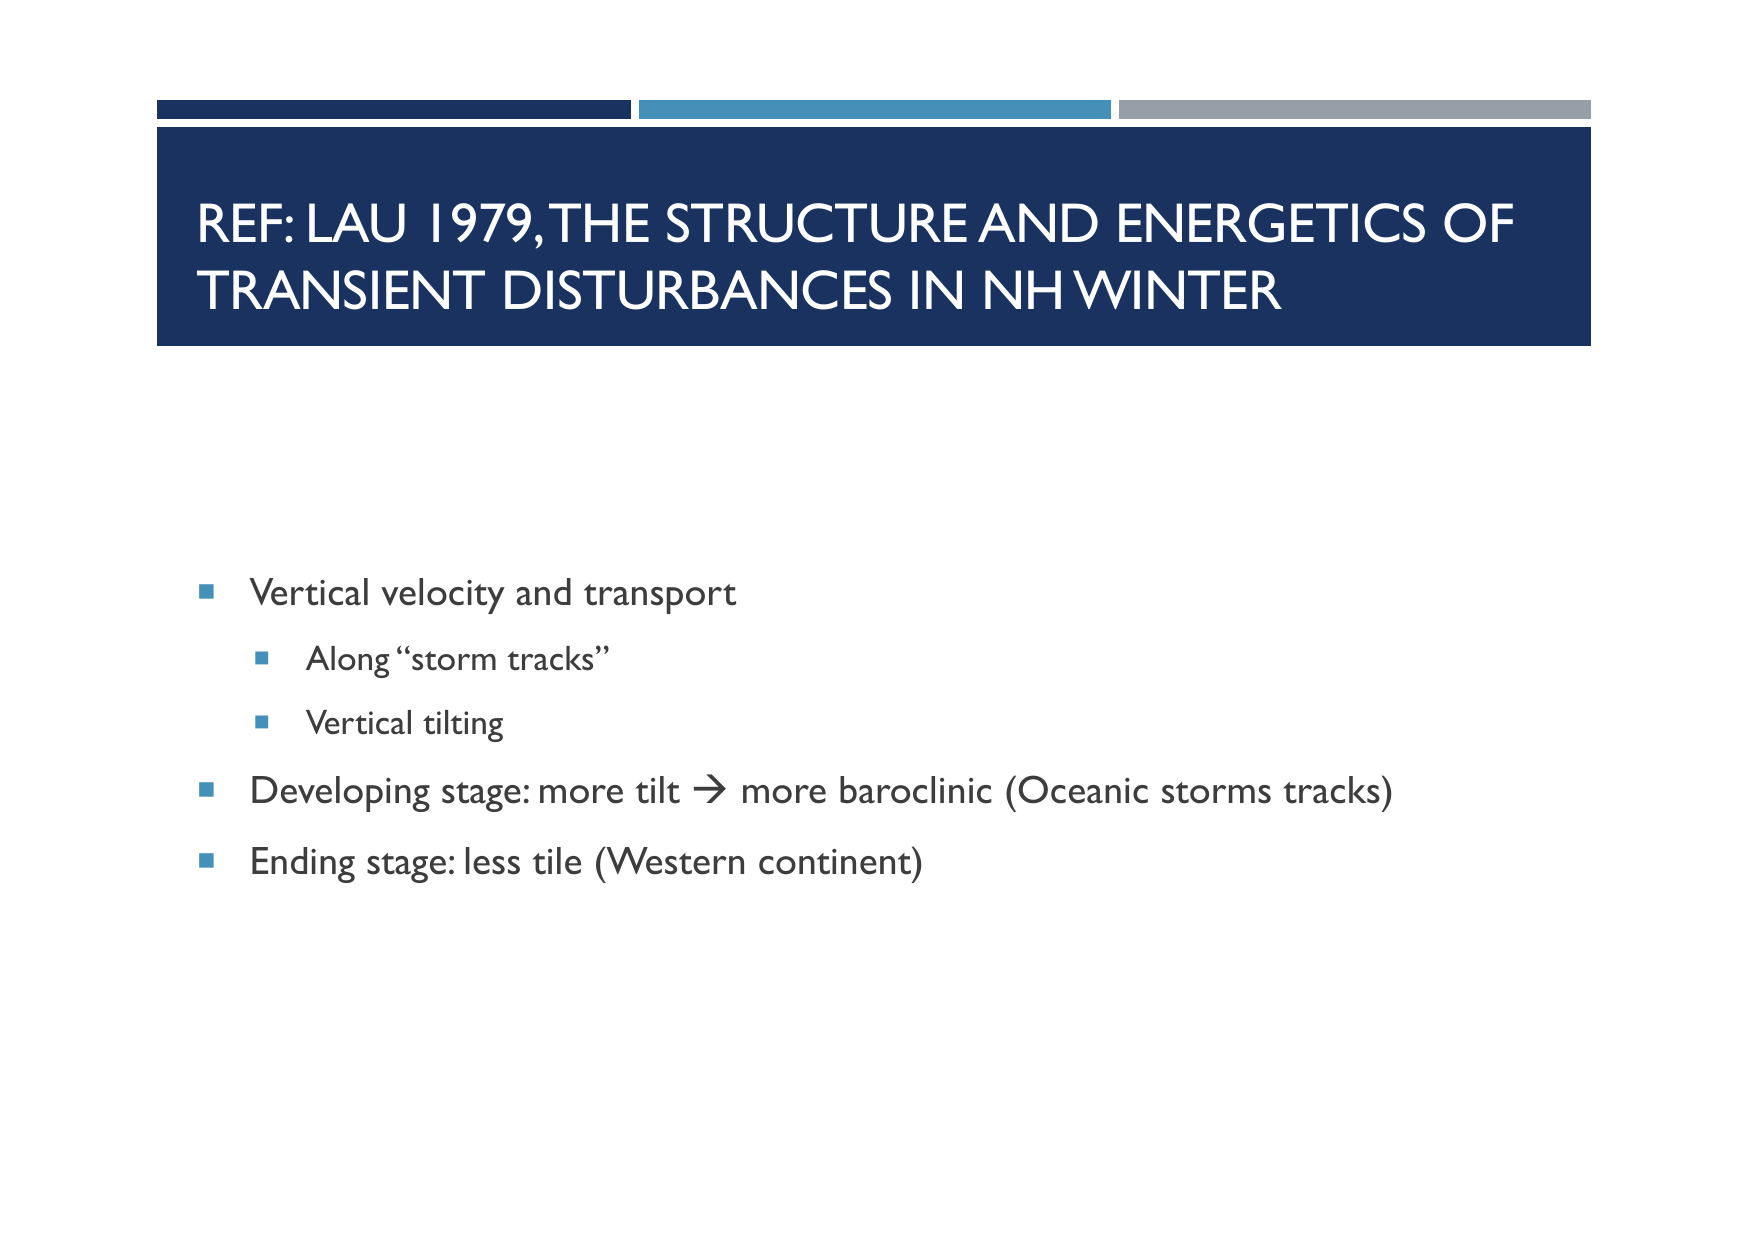
\includegraphics[width=0.85\textwidth]{images/ch06/p16_img01.png}
  \caption{Time-mean $\overline{\omega}(500\,\text{hPa})$ (top) and its band-pass
  standard deviation $\sigma_{\omega'}$ (bottom) for DJF.  The mean field is
  weak and spatially smooth, while the variability is sharply concentrated
  over the Pacific and Atlantic storm tracks.  This contrast shows that
  transient disturbances --- not the mean circulation --- are the dominant
  contributors to mid-tropospheric vertical motion in mid-latitudes.
  \hisu{시간 평균 $\omega$는 약하지만 표준편차는 storm track 위에서
  매우 크다.  중위도 연직운동은 평균 순환이 아니라 transient eddy가 주도한다.}}
  \label{fig:ch06_te_omega500_djf}
\end{figure}

\begin{definition}[Transient Vertical Velocity Variance]\label{def:ch06_te_omega_var}
For any field $a$ decomposed as $a = \overline{a} + a'$ where $\overline{(\cdot)}$
denotes a time mean (typically seasonal mean), the \textgr{transient variance}
of vertical velocity is
\[
  \sigma_{\omega'}^2 \equiv \overline{\omega'^2}
  = \overline{\omega^2} - \overline{\omega}^2.
\]
Large values of $\sigma_{\omega'}$ delineate regions where time-mean fields
are inadequate descriptions of the local circulation.
\end{definition}

\hisu{표준편차가 크다는 것은 시간 평균만으로는 그 지역의 대기를 설명할 수 없다는 뜻.
그래서 transient eddy를 따로 진단해야 한다.}

\begin{figure}[ht]
  \centering
  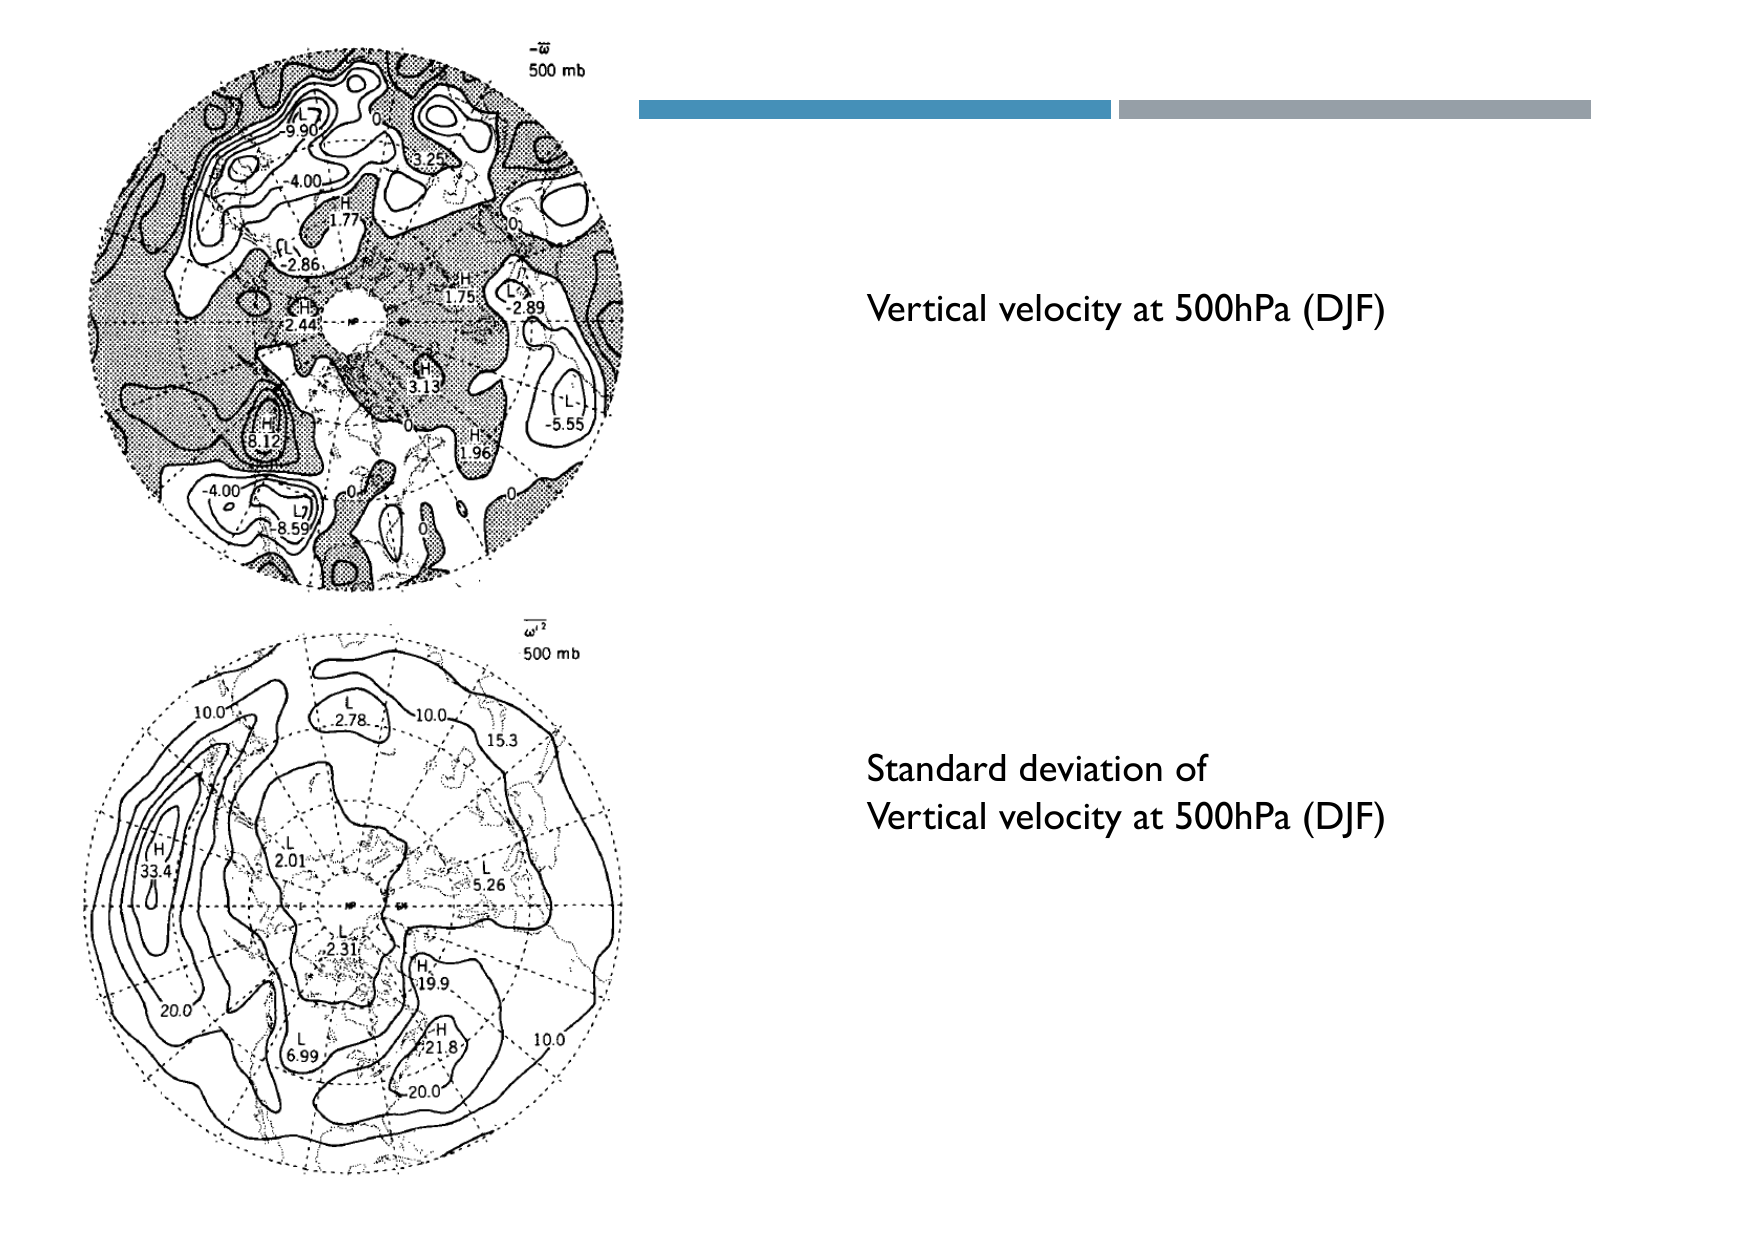
\includegraphics[width=0.85\textwidth]{images/ch06/p17_img01.png}
  \caption{Composite structure of synoptic-scale transient temperature
  fluctuations at $300\,\text{hPa}$ (top) and $700\,\text{hPa}$ (bottom) for
  DJF, after Lau (1979).  Note the characteristic spatial co-location of
  warm and cold anomalies with the storm-track regions, but with a small
  westward shift of the upper-tropospheric anomalies relative to those at
  $700\,\text{hPa}$.  \hisu{상층 ($300\,\text{hPa}$)의 온도 편차가
  하층 ($700\,\text{hPa}$)에 비해 서쪽으로 약간 밀려 있다.
  이 ``서쪽으로 기울어진 연직 구조''가 바로 baroclinic growth의 표식이다.}}
  \label{fig:ch06_te_T_300_700}
\end{figure}

\begin{remark}[Why $\omega$ and not $w$?]
Pressure-coordinate vertical velocity $\omega = Dp/Dt$ has the opposite sign
of geometric $w$ (upward $w$ corresponds to $\omega<0$).  In synoptic
practice $\omega$ at $500\,\text{hPa}$ is the canonical measure of large-scale
vertical motion because it appears directly in the QG omega equation and is
easily diagnosed from radiosonde divergence.
\end{remark}

\hisu{상층 발산이 강하면 $\omega < 0$ (상승), 수렴이 강하면 $\omega > 0$ (하강).
하층 폭풍의 warm sector 위에서 일관되게 $\omega < 0$이 나타난다.}

% =============================================================================
%   §2.2  Developing and Decaying Stages
% =============================================================================

\subsubsection{Developing and Decaying Stages}

이번에는 storm의 \textit{life cycle}에 따른 연직 구조 변화를 살펴본다.
관측과 idealized model이 일치하여 보여주는 가장 중요한 사실은,
\textgr{developing stage}의 polar front cyclone은 연직 방향으로
서쪽으로 강하게 기울어져 (\textgr{westward phase tilt with height}) 있으며,
\textgr{decaying (mature/occluded) stage}에서는 그 기울기가 점차 사라져
수직 정렬 (\textgr{vertical alignment})로 수렴한다는 점이다.

\begin{figure}[ht]
  \centering
  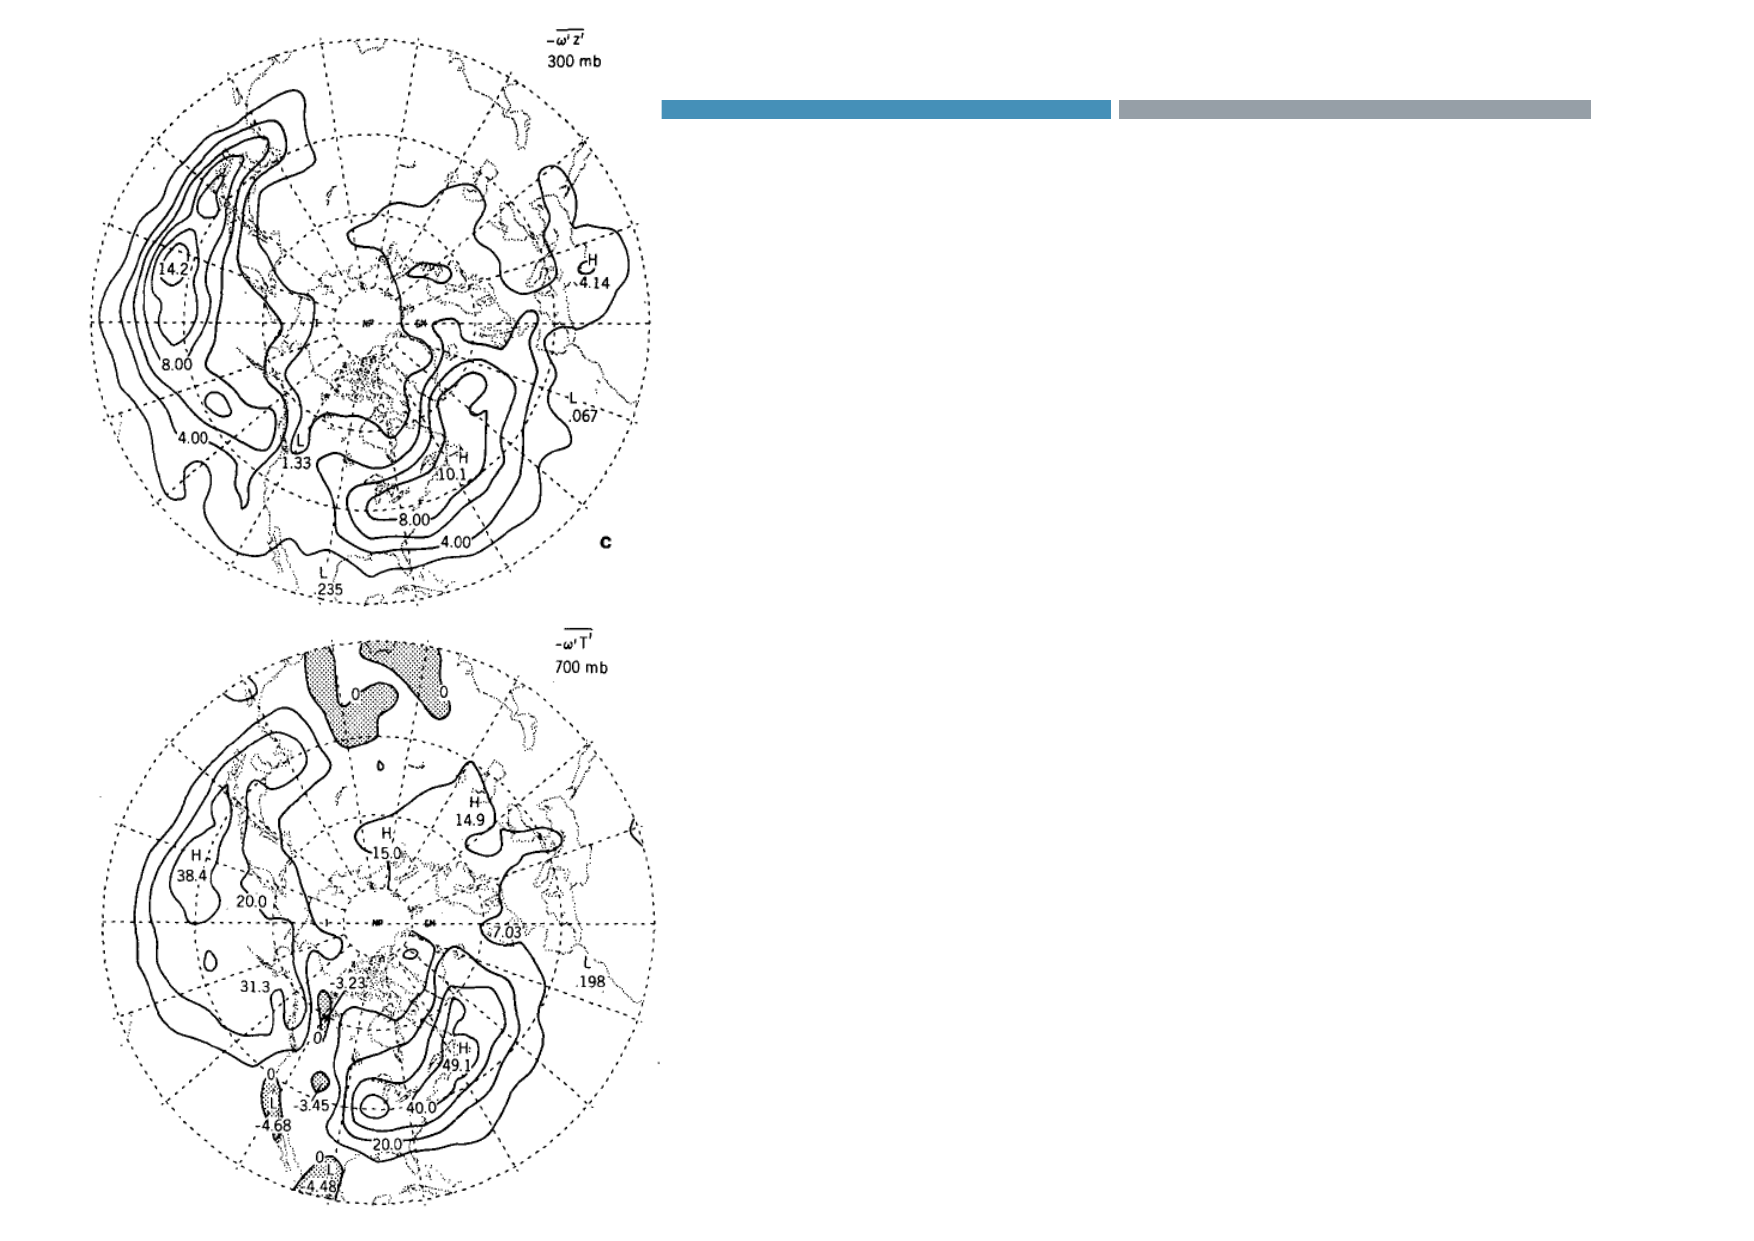
\includegraphics[width=0.85\textwidth]{images/ch06/p18_img01.png}
  \caption{Vertical cross-section (longitude--pressure) of a developing
  baroclinic disturbance.  Solid lines: geopotential height anomalies
  (trough/ridge); dashed lines: temperature anomalies (WARM, COLD); arrows:
  $\omega$ vector.  The upper-level trough is located \textbf{west of} the
  surface trough, and the warm anomaly is east of the surface low.  The
  resulting configuration places rising motion ($\omega<0$) over warm air
  and sinking motion ($\omega>0$) over cold air.  \hisu{발달기에는 상층
  trough가 지상 trough보다 서쪽에 위치한다.  warm air 위에서 상승,
  cold air 위에서 하강이 일어나 가용 위치 에너지가 운동 에너지로 변환된다.}}
  \label{fig:ch06_te_developing_xsec}
\end{figure}

\begin{theorem}[Westward Tilt and Baroclinic Energy Conversion]
\label{thm:ch06_te_tilt}
For a quasi-geostrophic wave of zonal wavenumber $k$ riding on a
vertically-sheared zonal flow $\overline{u}(p)$ with
$\partial \overline{u}/\partial p < 0$ (westerly shear with height),
the wave grows in time \emph{if and only if} its geopotential perturbation
$\Phi'$ tilts westward with height, i.e.\ the upper-level pressure trough
lies upstream (west) of the lower-level pressure trough.  Equivalently, the
poleward eddy heat flux satisfies
\[
  \overline{v'T'} > 0
  \quad\Longleftrightarrow\quad
  \text{westward phase tilt with height}.
\]
\end{theorem}

\begin{hisublock}
이 정리는 Holton \& Hakim (2012) Ch.~8 (baroclinic instability)의
Eady model과 Charney model에서 유도되는 결과이다.  Eady model에서는
edge wave가 $-\pi/2 < \theta < 0$ 범위의 phase shift를 가질 때 성장한다.
물리적으로는 (i) eddy가 warm air를 북쪽으로, cold air를 남쪽으로 수송하여
($\overline{v'T'}>0$) 평균 자오선 온도 경도를 약화시키고,
(ii) 그 줄어든 APE가 eddy의 $K_T$로 변환된다.
즉 \textbf{서쪽 기울기 = 양의 자오선 열 플럭스 = baroclinic growth}의
삼위일체이다.
\end{hisublock}

\begin{figure}[ht]
  \centering
  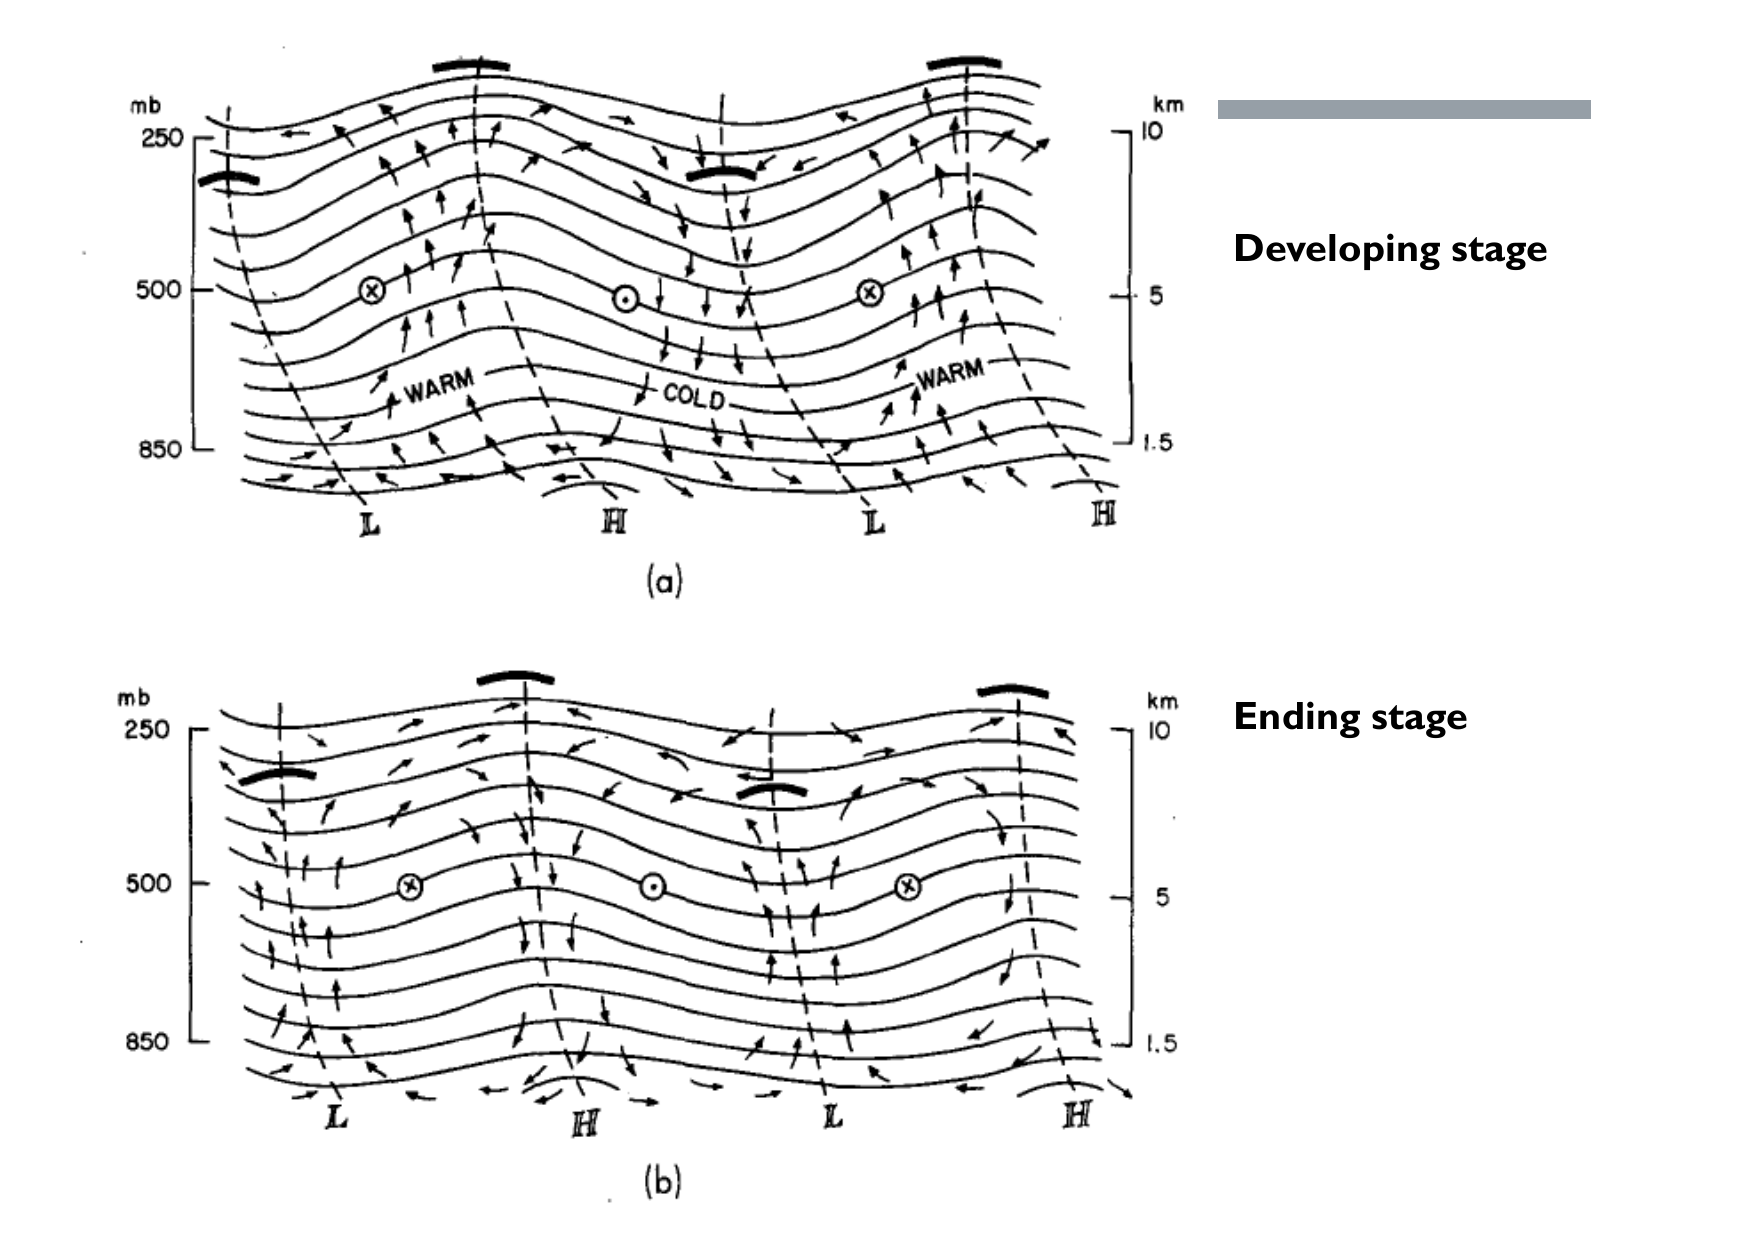
\includegraphics[width=0.85\textwidth]{images/ch06/p19_img01.png}
  \caption{Same as Fig.~\ref{fig:ch06_te_developing_xsec} but for the
  decaying (occluded) stage.  The vertical tilt has largely disappeared:
  upper and surface troughs are nearly co-located, warm and cold anomalies
  have wrapped around the surface low, and the $\omega$ couplet has
  weakened.  \hisu{쇠퇴기에는 상하층 trough가 거의 일직선상에 정렬되어
  baroclinic conversion이 멈춘다.  이제 폭풍은 마찰과 확산에 의해
  소산된다.}}
  \label{fig:ch06_te_decaying_xsec}
\end{figure}

\begin{remark}[Lifecycle Interpretation]
The transition from developing to decaying state is the canonical
nonlinear lifecycle of a baroclinic eddy (Simmons \& Hoskins, 1978):
the wave first extracts $K_T$ from the mean flow via westward tilt,
saturates as the tilt collapses, and ultimately deposits its energy
back into the zonal flow at upper levels (\emph{barotropic decay}).
\end{remark}

\hisu{발달기에는 평균에서 에디로, 쇠퇴기에는 에디에서 평균으로 ---
이것이 baroclinic life cycle의 ``쌍방향 에너지 흐름''이다.}

% =============================================================================
%   §2.3  The Kinetic Energy Budget
% =============================================================================

\subsubsection{The Kinetic Energy Budget}

앞의 정성적 그림을 정량화하기 위해 \textgr{kinetic energy (KE) budget}을
구성한다.  속도장을 $\mathbf{V} = \overline{\mathbf{V}} + \mathbf{V}'$로
분해하면 ($\overline{(\cdot)}$는 시간 평균),
평균 운동 에너지와 transient 운동 에너지를 각각 다음과 같이 정의한다.

\begin{definition}[Mean and Transient Kinetic Energy]\label{def:ch06_te_KE}
\begin{align}
  \overline{K_M}
    &\equiv \tfrac{1}{2}\left(\overline{u}^2 + \overline{v}^2\right),
    \label{eq:ch06_te_KM_def}\\
  K_T
    &\equiv \tfrac{1}{2}\,\overline{u'^2 + v'^2}.
    \label{eq:ch06_te_KT_def}
\end{align}
$\overline{K_M}$은 시간 평균 흐름 자체의 운동 에너지이며,
$K_T$는 시간 평균 흐름으로부터 편차의 분산 (즉 transient eddy의
운동 에너지)이다.
\end{definition}

\hisu{강의 슬라이드에 $K_T = \tfrac{1}{2}\overline{(u'^2 v'^2)}$로 표기된 부분이
있는데 이는 명백한 typo이다.  올바른 표기는 $\tfrac{1}{2}\overline{(u'^2+v'^2)}$.}

각각의 시간 진화 방정식을 NS 방정식과 시간평균/편차 분해로부터 유도하면
다음과 같다.  자세한 유도는 Holton \& Hakim (2012) Ch.~10 또는
Peixoto \& Oort (1992) Ch.~13을 참조하라.

\begin{theorem}[Mean and Transient KE Equations]\label{thm:ch06_te_KE_budget}
\begin{align}
  \frac{\partial \overline{K_M}}{\partial t}
    &= -\nabla\!\cdot\!\bigl(H_0 + H_1\bigr)
       - \frac{\partial}{\partial p}\!\left[\overline{K_M}\,\overline{\omega}
         + \overline{(\overline{u'v'} + \overline{v'u'})\,\omega'}\right]
       \nonumber\\
    &\quad
       - \overline{\mathbf{V}}\cdot\nabla\overline{\Phi}
       + \overline{\mathbf{V}}\cdot\overline{\mathbf{F}}
       - C\!\bigl(\overline{K_M},\,K_T\bigr),
       \label{eq:ch06_te_KM_eq}\\[4pt]
  \frac{\partial K_T}{\partial t}
    &= -\nabla\!\cdot\!\bigl(H_2 + H_3\bigr)
       - \frac{\partial}{\partial p}\!\left(K_T\,\overline{\omega}\right)
       \nonumber\\
    &\quad
       - \overline{\mathbf{V}'\!\cdot\nabla\Phi'}
       + \overline{\mathbf{V}'\!\cdot\mathbf{F}'}
       + C\!\bigl(\overline{K_M},\,K_T\bigr),
       \label{eq:ch06_te_KT_eq}
\end{align}
where the four horizontal flux terms are defined as
\begin{align}
  H_0 &= \overline{\mathbf{V}}\;\overline{K_M},
    \label{eq:ch06_te_H0}\\
  H_1 &= \overline{\bigl(\overline{u'v'} + \overline{v'u'}\bigr)\,\omega'},
    \label{eq:ch06_te_H1}\\
  H_2 &= \overline{\mathbf{V}'}\,K_T,
    \label{eq:ch06_te_H2}\\
  H_3 &= \tfrac{1}{2}\,\overline{(u'^2 + v'^2)\,v'}.
    \label{eq:ch06_te_H3}
\end{align}
The cross-term $C(\overline{K_M},K_T)$ is the \textgr{barotropic conversion}
between mean and eddy KE.
\end{theorem}

\begin{hisublock}
네 개의 수송 항 $H_0$--$H_3$의 물리적 의미를 한 줄씩 정리하면:
\begin{itemize}
  \item $H_0 = \overline{\mathbf{V}}\,\overline{K_M}$:
        평균 흐름이 \emph{스스로의} KE를 advect.
        대규모 jet에 의한 KE 재분배가 여기에 들어간다.
  \item $H_1 = \overline{(\overline{u'v'}+\overline{v'u'})\omega'}$:
        eddy 운동량 플럭스가 \emph{eddy 연직속도} $\omega'$와 결합되어
        만드는 cross-correlation.  jet streak 부근에서 두드러진다.
  \item $H_2 = \overline{\mathbf{V}'}\,K_T$:
        eddy meridional 흐름 $\overline{\mathbf{V}'}$ (즉 시간 평균이 아닌
        eddy 자체의 평균)이 $K_T$를 운반.  실제로는 보통 작다.
  \item $H_3 = \tfrac{1}{2}\,\overline{(u'^2+v'^2)v'}$:
        eddy가 \emph{자기 자신의} KE를 자오선 방향으로 self-transport.
        storm track에서 가장 중요한 항.
\end{itemize}
이 분해는 Lau (1979a)의 Eqs.~(2)--(3)에 대응하며, NCEP/NCAR reanalysis
기반 진단치는 그의 Fig.~6 (300 hPa)에서 확인할 수 있다.
\end{hisublock}

\begin{remark}[Sign Convention of $C(\overline{K_M},K_T)$]
\label{rem:ch06_te_CKMKT_sign}
By construction
\[
  C\!\bigl(\overline{K_M},\,K_T\bigr)
  = -\,\overline{u'v'}\frac{\partial \overline{u}}{\partial y}
    -\,\overline{u'\omega'}\frac{\partial \overline{u}}{\partial p}
    + \text{(meridional analogues)},
\]
so that the same term enters \eqref{eq:ch06_te_KM_eq} with a \emph{minus}
sign and \eqref{eq:ch06_te_KT_eq} with a \emph{plus} sign.  Therefore
\[
  C\!\bigl(\overline{K_M},\,K_T\bigr) > 0
  \quad\Longleftrightarrow\quad
  \text{mean KE is being drained to feed eddies.}
\]
\end{remark}

\hisu{핵심: $C > 0$이면 평균 흐름이 운동 에너지를 잃고 에디가 얻는다.
이것이 \textbf{baroclinic instability의 운동학적 정의}이다.
중위도 storm track에서 일관되게 $C > 0$이 관측된다.}

\begin{example}[Typical Magnitudes]\label{ex:ch06_te_magnitudes}
DJF 평균 NH mid-latitude jet level (300 hPa) 에서의 관측치 (Lau, 1979a;
Peixoto \& Oort, 1992 Table~13.1):
\begin{itemize}
  \item Mean KE: $\overline{K_M} \approx 250\text{--}400\;\text{m}^2/\text{s}^2$
        (jet core에서 최대).
  \item Transient KE: $K_T \approx 80\text{--}150\;\text{m}^2/\text{s}^2$
        (storm track에서 최대; jet core의 $\sim$$30$--$40\%$).
  \item Vertically integrated barotropic conversion:
        $C(\overline{K_M},K_T) \approx 0.5\text{--}1.5\;\text{W}/\text{m}^2$
        in the storm-track core.
  \item Self-transport flux: $H_3$의 zonal 평균 자오선 성분
        $\sim 5\text{--}10\;\text{m}^2/\text{s}^2 \cdot \text{m/s}$
        (poleward of $40^\circ\text{N}$에서 적도 방향, equatorward에서 극 방향
        --- 즉 storm track latitude에서 발산).
\end{itemize}
\end{example}

\hisu{Storm track의 KE는 평균 jet의 약 30--40\% 정도.
$C(\overline{K_M},K_T)$가 약 $1\,\text{W/m}^2$이므로,
$K_T$가 $100\,\text{m}^2/\text{s}^2$이라면 $e$-folding time이
$10^5\,\text{s} \approx 1\,\text{day}$ --- 관측된 baroclinic eddy의
성장률과 일치!}

\begin{remark}[Why Four Transports?]\label{rem:ch06_te_four_H}
Each $H_i$ corresponds to a distinct physical pathway:
\begin{itemize}
  \item $H_0$: \emph{mean by mean} (no eddy involvement),
  \item $H_1$: \emph{mean--eddy} cross (eddy momentum transported by mean $\omega'$
        and stretched by mean field),
  \item $H_2, H_3$: \emph{eddy by eddy} (self-transport and triple correlation).
\end{itemize}
이러한 4-term decomposition은 에너지 cycle의 generation, transport,
dissipation을 별도로 진단할 수 있게 해 준다.  Lau (1979a) Tables~1--2
에서는 각 항을 격자별로 평가하여, storm track entrance 영역에서
$C > 0$ (eddy 성장), exit 영역에서 $\nabla\cdot H_3$ 발산 (eddy KE
배출)이 명확히 분리됨을 보였다.
\end{remark}

% =============================================================================
%   §2.4  Energy Cycle Diagram
% =============================================================================

\subsubsection{Energy Cycle Diagram}

위의 KE budget을 도식적으로 정리하면 Lorenz (1955)의 고전적
\textgr{atmospheric energy cycle} 그림이 얻어진다.

\begin{figure}[ht]
  \centering
  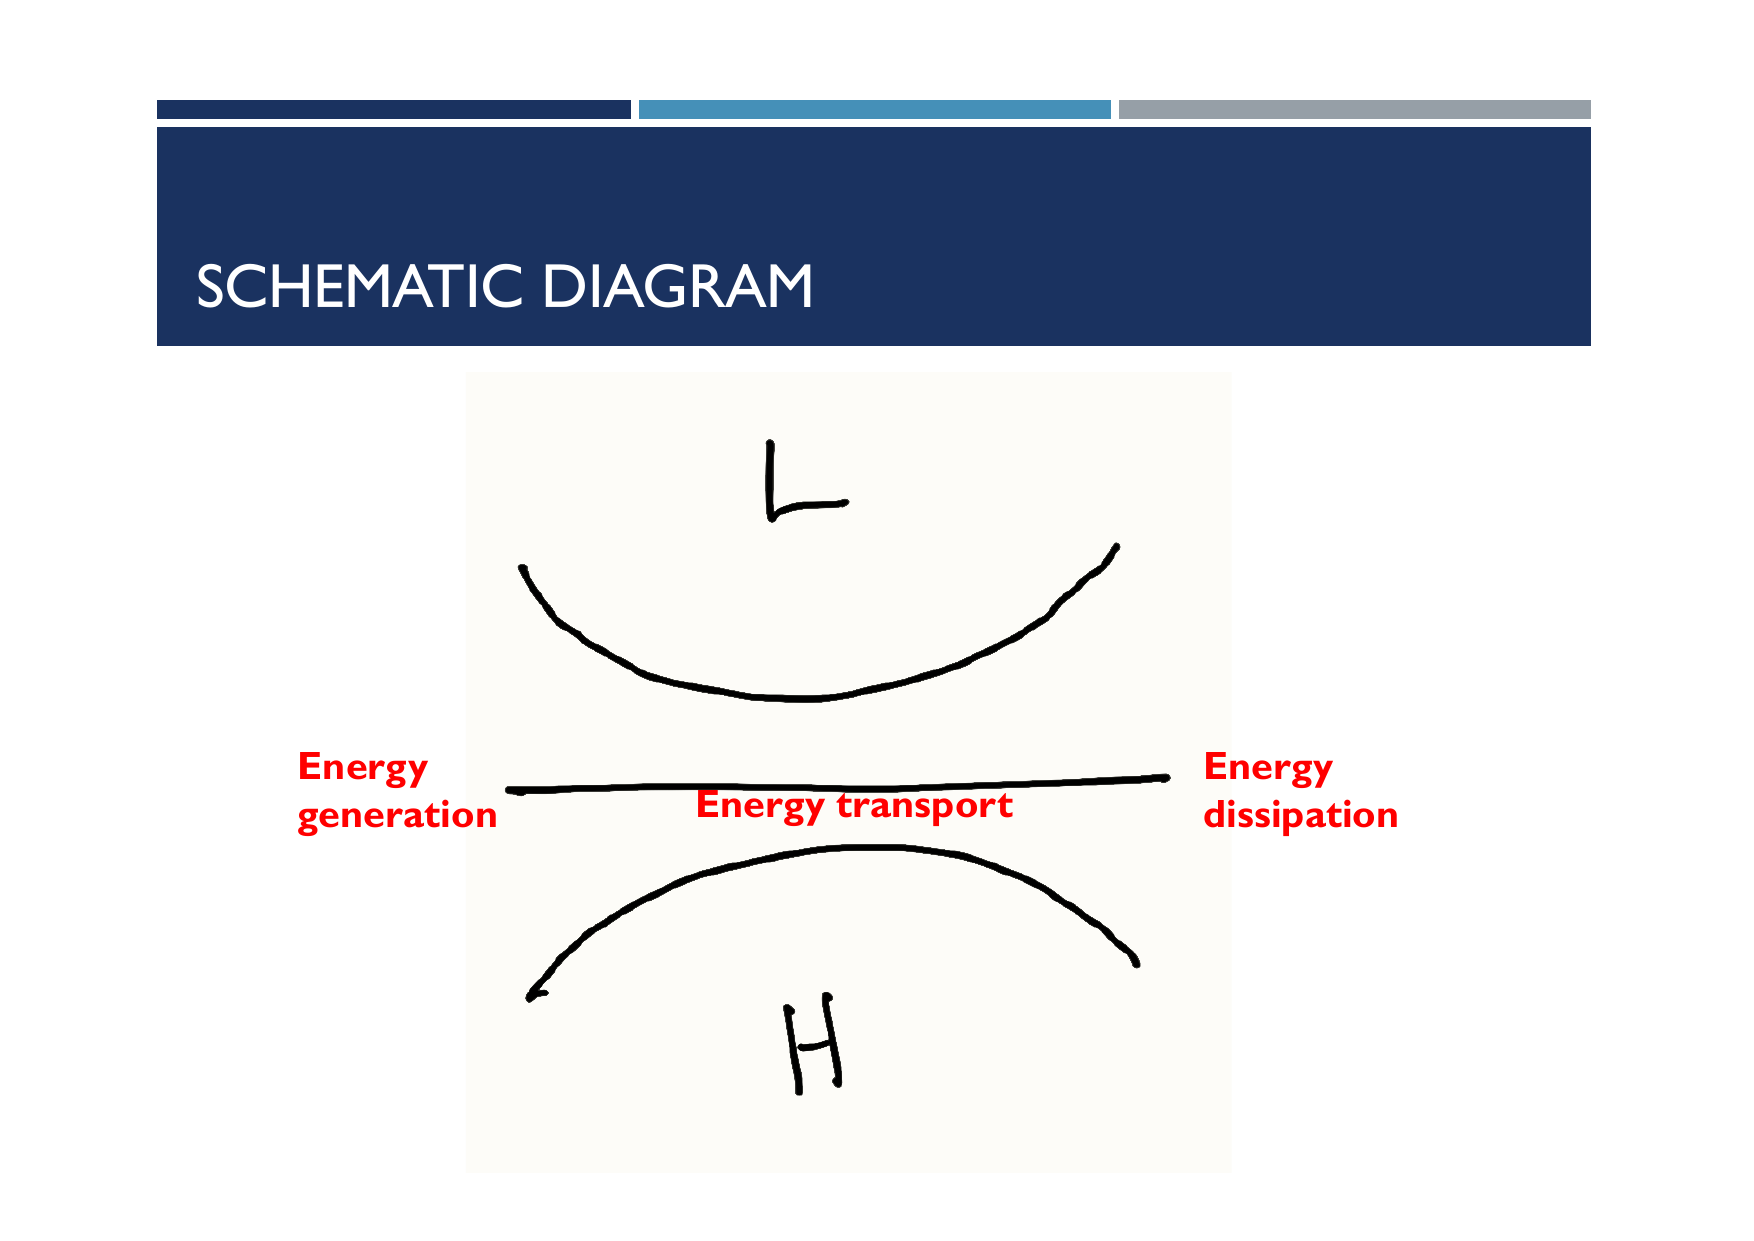
\includegraphics[width=0.85\textwidth]{images/ch06/p22_img01.png}
  \caption{Schematic atmospheric energy cycle following Lorenz (1955),
  adapted for the mean--transient partition discussed in
  Theorem~\ref{thm:ch06_te_KE_budget}.  The four reservoirs are mean
  available potential energy ($\overline{P_M}$), transient available
  potential energy ($P_T$), mean kinetic energy ($\overline{K_M}$), and
  transient kinetic energy ($K_T$).  Arrows show the dominant pathways:
  diabatic generation $G_M$ creates $\overline{P_M}$;
  baroclinic conversion $C(\overline{P_M},P_T)$ via $\overline{v'T'}>0$
  transfers it to $P_T$;
  adiabatic conversion $C(P_T,K_T)$ via $-\overline{\omega'T'}>0$ feeds
  storm KE;
  barotropic conversion $C(\overline{K_M},K_T)$ in
  \eqref{eq:ch06_te_KM_eq}--\eqref{eq:ch06_te_KT_eq} closes the loop;
  frictional dissipations $D_M$ and $D_T$ ultimately remove KE.
  \hisu{대기 에너지의 4-box cycle. 화살표의 방향이 양수이면
  baroclinic instability에 의한 ``정상'' eddy 성장이고,
  반대 방향은 ``barotropic decay''에 해당한다.}}
  \label{fig:ch06_te_lorenz_cycle}
\end{figure}

\begin{hisublock}
이 cycle을 본문 \eqref{eq:ch06_te_KM_eq}--\eqref{eq:ch06_te_KT_eq}와
연결하면 다음과 같다:
\begin{itemize}
  \item $G_M$ (diabatic generation of $\overline{P_M}$): 적도--극 차등 가열.
        평균 자오선 온도 경도를 유지하는 원동력.
  \item $C(\overline{P_M},P_T)$: $\overline{v'T'}>0$
        (즉 westward-tilted eddy)에 의한 $\overline{P_M}\to P_T$ 변환.
        Theorem~\ref{thm:ch06_te_tilt}에서 본 것이 바로 이 항.
  \item $C(P_T,K_T)$: $-\overline{\omega'T'}>0$
        (warm air rises, cold air sinks)에 의한 $P_T\to K_T$ 변환.
        Section~\ref{fig:ch06_te_developing_xsec}의 schematic이 이를 보여준다.
  \item $C(\overline{K_M},K_T)$: 본문 \eqref{eq:ch06_te_KM_eq}의 마지막 항.
        Storm track 입구에서 양수, 출구에서 음수 (Lau 1979a Fig.~6).
  \item $D_M,\,D_T$: surface friction (Ekman dissipation)에 의한 KE 손실.
\end{itemize}
\textbf{4-term decomposition} ($H_0,\dots,H_3$)은 위 화살표 중
\textbf{transport} (즉 cycle 안에서의 에너지 \textit{재분배})를
공간적으로 정량화한 것이다.  Generation은 외부 입력 ($\dot{Q}$),
dissipation은 외부 방출 ($\mathbf{F}$), 그 사이의 redistribution이 $H_i$.
\end{hisublock}

\hisu{Lorenz cycle의 4개 박스가 어떻게 닫히는가:
태양 가열이 $\overline{P_M}$을 만들고, baroclinic eddy가 이를
$P_T \to K_T \to \overline{K_M}$ (또는 마찰로 소산)으로 변환한다.
$H_0$--$H_3$는 이 cycle의 ``공간적 흐름''을 표현한다.}

% =============================================================================
%   §2.5  Summary: Stationary vs Transient Contrast
% =============================================================================

\subsubsection{Summary: Stationary vs Transient Contrast}

\S2를 마무리하기에 앞서, transient eddy 와 \S3에서 다룰 stationary wave를
한 표로 대비한다.  두 component는 \textit{같은} 시간 평균 비대칭 (asymmetric
circulation)을 함께 구성하지만, 물리적 메커니즘과 지리적 분포가 매우 다르다.

\begin{table}[ht]
  \centering
  \begin{tabular}{p{0.28\textwidth}p{0.32\textwidth}p{0.32\textwidth}}
    \hline
    \textbf{Property}
      & \textbf{Transient eddies (\S2)}
      & \textbf{Stationary waves (\S3)} \\
    \hline
    Definition
      & Departures from time mean
      & Time-mean departures from zonal mean \\
    Timescale
      & $2$--$10$ days (synoptic)
      & Effectively infinite (DJF mean) \\
    Spatial signature
      & Concentrated in \textgr{storm tracks} (Pacific, Atlantic)
      & Locked to \textgr{forcing} (orography, land--sea heating) \\
    Vertical structure
      & Westward tilt with height (developing)
      & Equivalent-barotropic in extratropics \\
    Energy source
      & Baroclinic conversion $C(\overline{P_M},P_T)$, $C(\overline{K_M},K_T)$
      & Quasi-stationary forcing (mountain torque, diabatic heat) \\
    Local maintenance of KE
      & Dominant in storm-track regions
      & Dominant in continental and orographic regions \\
    Key flux signature
      & $\overline{v'T'}>0$, westward tilt
      & $\overline{v}_E\,\overline{T}_E \neq 0$, $\overline{u}_E\,\overline{v}_E \neq 0$ \\
    Reference figure
      & Fig.~\ref{fig:ch06_te_developing_xsec},
        Fig.~\ref{fig:ch06_te_decaying_xsec}
      & to follow in \S3 \\
    \hline
  \end{tabular}
  \caption{Contrast between transient eddies and stationary waves as
  contributors to the zonally asymmetric general circulation.
  \hisu{시간 스케일과 강제 메커니즘이 다른 두 ``비대칭 성분''의 비교표.
  Storm track은 transient의 영역, 산악/대륙 효과는 stationary의 영역.}}
  \label{tab:ch06_te_vs_stationary}
\end{table}

\begin{remark}[Why both matter]
관측된 시간 평균 비대칭 ($Z_E$, $T_E$, $u_E$, $v_E$)은 stationary 성분만
포함하므로, ``time mean이 어떻게 유지되는가?''를 따질 때 transient eddy의
flux convergence가 forcing 역할을 한다 (\S3.27의 vorticity budget,
\S3.30의 heat budget 참조).  따라서 \S3의 stationary wave 진단은
\S2에서 구축한 transient eddy 통계 위에 세워진다.
\end{remark}

\hisu{시간 평균의 ``파동'' = stationary wave.  그 평균이 \textit{유지되도록}
운동량과 열을 공급하는 것 = transient eddy.  두 성분은 서로 보완적이지
독립이 아니다.}

\begin{hisublock}
\textbf{§2 한국어 요약 정리}:
\begin{enumerate}
  \item \textbf{관측 사실}: storm track 위에서 $\sigma_{\omega'}$,
        $\sigma_{T'}$, $\sigma_{Z'}$ 모두 극대.  시간 평균이 아니라
        transient eddy가 중위도 대류권을 지배한다
        (Fig.~\ref{fig:ch06_te_omega500_djf}).
  \item \textbf{연직 구조}: developing stage에서는 상층 trough가 하층
        trough보다 \textit{서쪽}에 위치 (westward tilt with height).
        이 tilt가 양의 자오선 열 플럭스 $\overline{v'T'}>0$를 만들고
        baroclinic growth를 일으킨다
        (Fig.~\ref{fig:ch06_te_developing_xsec},
        Theorem~\ref{thm:ch06_te_tilt}).
  \item \textbf{Decaying stage}: tilt가 사라지고 상하층이 수직 정렬되면
        baroclinic conversion이 멈추고 폭풍은 소산된다
        (Fig.~\ref{fig:ch06_te_decaying_xsec}).
  \item \textbf{KE budget}: $\overline{K_M}$과 $K_T$의 진화 방정식은
        4개의 수송 항 $H_0,H_1,H_2,H_3$과 cross-term
        $C(\overline{K_M},K_T)$로 닫힌다
        (Theorem~\ref{thm:ch06_te_KE_budget}).
        $C > 0$이면 mean $\to$ eddy 에너지 흐름 = baroclinic
        instability.
  \item \textbf{에너지 cycle}: Lorenz 4-box diagram이 전체 cycle을
        통합 (Fig.~\ref{fig:ch06_te_lorenz_cycle}).
        $G \to \overline{P_M} \to P_T \to K_T \to \overline{K_M} \to D$.
\end{enumerate}

\medskip
\textbf{§3로의 연결}: \S2에서 본 transient eddy는 그 자체로 중요하지만,
시간 평균 자체의 비대칭 (= stationary wave)을 \textit{유지}하는 역할도
한다.  \S3에서는 stationary wave의 3차원 구조를 진단하고, vorticity
budget과 heat budget을 통해 그 local maintenance를 정량화한다.
표~\ref{tab:ch06_te_vs_stationary}는 두 component의 차이를 미리 정리한
것이다.
\end{hisublock}
% =============================================================================
%   Chapter 6, Section 3: Structure of Tropospheric Stationary Waves
%                          and Local Maintenance
%   Based on Ch06 lecture notes p.24-41
%   Primary reference: Lau (1979a, 1979b), Held (1983)
% =============================================================================

\subsection{Structure of Tropospheric Stationary Waves and Local Maintenance}\label{subsec:ch06_stationary}

§1과 §2에서 우리는 북반구 겨울철 순환의 zonally asymmetric 특성을 관측적으로 살펴보고,
이를 \textgr{transient eddies}(시간 평균에서의 편차)와 \textgr{stationary eddies}(지역적으로 고정된 시간 평균 비대칭)
두 성분으로 분해할 수 있음을 확인했다.
§3에서는 후자인 \textbf{tropospheric stationary waves}의 3차원 구조와,
그것이 \textgr{local maintenance}---즉 어떻게 한 지점에서 운동량·열·운동에너지가 균형을 이루며 유지되는지---를
어떻게 결정하는지를 본격적으로 분석한다.

핵심 통찰은 다음과 같다: 시간 분산(variance)의 관점에서는 transient eddies가 지배적이지만,
운동량·열·운동에너지의 \emph{지역적} 평균값을 유지하는 데에는 stationary eddies가 결정적 역할을 한다.
이 절에서는 Q-G vorticity balance, 시간 평균 vertical motion, heat budget,
rotational/divergent wind decomposition, 그리고 streamfunction과 velocity potential 사이의
\textbf{quarter-phase shift theorem}을 차례로 다루며,
마지막으로 Lau (1979)의 관측 단면도를 통해 stationary wave의 3차원 구조를 직접 확인한다.

\hisu{핵심 질문 한 줄: \emph{왜 stationary eddies가 평균 순환의 지역적 유지에 결정적인가?}}

% --------------------------------------------------------------------------
\subsubsection{Introduction: 3D Structure of Stationary Waves}
% --------------------------------------------------------------------------

\textbf{Lau (1979)}의 두 편의 논문(\textit{J. Atmos. Sci.}, vorticity/heat balance와 energetics)은
북반구 겨울철 stationary eddies의 3차원 구조를 NMC analyses에 근거해 처음으로 체계적으로 기술했다.
이 분석은 위도대별로 매우 다른 양상을 드러낸다.

\begin{itemize}
  \item \textgr{High latitudes} ($\sim 60^\circ$N): stationary eddies가 대류권 상층에서 \emph{성층권으로}
        에너지를 능동적으로 수송한다. 즉 stratosphere--troposphere coupling의 주된 통로다.
  \item \textgr{Mid-latitudes} ($\sim 45^\circ$N): 상층 대류권(200--300 hPa)에서 에너지 수송이 최대가 된다.
        Jet stream과 storm track의 동측에서 stationary wave의 진폭과 활동도가 정점에 도달한다.
  \item \textgr{Tropics} ($\sim 25^\circ$N 이남): 진폭은 작지만 mid-latitudes의 stationary wave와
        독특한 \emph{phase relationship}을 갖는다. Walker circulation과 monsoon system이
        이 위도대 stationary signal의 주요 원천이다.
\end{itemize}

\hisu{위도에 따라 stationary wave의 역할이 다르다: 고위도는 성층권 결합, 중위도는 상층에서 최대,
열대는 phase 관계가 핵심이다.}

\begin{hisublock}
\textbf{Stationary vs.\ Transient — General Circulation Statistics 관점}.
강의 노트 p.~26과 Lau (1979b)의 Table~1에 정리된 NMC 데이터에 따르면,
\emph{시간 분산(temporal variance)}의 대부분은 transient eddies가 차지한다(특히 storm track 위도에서
$\overline{u'^2}, \overline{v'^2}, \overline{T'^2}$의 90\,\% 이상이 transient 성분).
그러나 \emph{시간 평균} 운동량 플럭스 $-\overline{V'u'}$, 열 플럭스 $\overline{v'T'}$,
운동에너지 변환을 \emph{지역적으로} 가중평균하면 stationary eddies의 기여가
mid-latitude 일부 지점에서 transient에 필적하거나 능가한다.
즉 ``평균 상태를 \textbf{어디서} 유지하는가''라는 질문에 대한 답은 stationary eddies가 쥐고 있다.

이 두 관점---variance dominance vs.\ local maintenance dominance---의 차이가
§3 전체의 출발점이다.
\end{hisublock}

% --------------------------------------------------------------------------
\subsubsection{Time-Average Vorticity Balance}
% --------------------------------------------------------------------------

Stationary wave 유지의 출발점은 \textgr{quasi-geostrophic vorticity equation}이다.
Ch.5에서 유도한 표준형은 다음과 같다:
\begin{equation}\label{eq:ch06_sw_qgvort}
  \frac{\partial \zeta_g}{\partial t}
  \;=\; f_0\,\frac{\partial \omega}{\partial p}
       \;-\; \mathbf{V}_g\!\cdot\!\nabla \zeta_g
       \;-\; \beta\, v_g .
\end{equation}
여기서 $\zeta_g = \hat{k}\!\cdot\!\nabla\times \mathbf{V}_g$는 relative geostrophic vorticity,
$\omega = Dp/Dt$는 pressure-coordinate vertical velocity,
$\beta = df/dy$는 행성 vorticity의 자오 기울기다.

\begin{definition}[Reynolds Decomposition for Stationary-Transient]\label{def:ch06_sw_reynolds}
임의의 변수 $A(\lambda,\phi,p,t)$를 long-term time mean $\overline{A}$와 편차 $A'$으로 분해한다:
\begin{equation}\label{eq:ch06_sw_decomp}
  A \;=\; \overline{A} \;+\; A',\qquad \overline{A'} \equiv 0 .
\end{equation}
여기서 overbar는 한 계절 이상의 \emph{시간} 평균을 의미하며, zonal 평균이 아니라는 점에 유의한다.
따라서 $\overline{A}(\lambda,\phi,p)$는 여전히 경도 의존성을 가지는 stationary 부분이다.
\end{definition}
\hisu{시간 평균 후에도 경도 의존성이 남아 있는 부분이 stationary eddy다.}

\eqref{eq:ch06_sw_qgvort}에 시간 평균을 취하면 $\partial \zeta_g/\partial t$의 long-term 평균은 0에 수렴하므로,
\begin{equation}\label{eq:ch06_sw_vorbal_raw}
  0 \;=\; f_0\,\frac{\partial \overline{\omega}}{\partial p}
       \;-\; \overline{\mathbf{V}_g\!\cdot\!\nabla \zeta_g}
       \;-\; \beta\, \overline{v}_g .
\end{equation}
이때 nonlinear advection $\overline{\mathbf{V}_g\!\cdot\!\nabla\zeta_g}$를 평균과 편차로 풀어쓰면
\begin{equation}\label{eq:ch06_sw_advdecomp}
  \overline{\mathbf{V}_g\!\cdot\!\nabla\zeta_g}
  \;=\; \overline{\mathbf{V}}_g\!\cdot\!\nabla \overline{\zeta}_g
       \;+\; \overline{\mathbf{V}_g'\!\cdot\!\nabla \zeta_g'} .
\end{equation}
편차 항은 비발산 흐름의 항등식 $\mathbf{V}_g\!\cdot\!\nabla\zeta_g = \nabla\!\cdot\!(\mathbf{V}_g\zeta_g) - \zeta_g\nabla\!\cdot\!\mathbf{V}_g$
와 $\nabla\!\cdot\!\mathbf{V}_g \approx 0$ (Q-G 근사)에 의해
\begin{equation}\label{eq:ch06_sw_eddyflux}
  \overline{\mathbf{V}_g'\!\cdot\!\nabla \zeta_g'}
  \;\approx\; \nabla\!\cdot\!\overline{\mathbf{V}_g'\,\zeta_g'}
\end{equation}
형태의 \textgr{transient vorticity flux convergence}로 표현된다.

\eqref{eq:ch06_sw_vorbal_raw}--\eqref{eq:ch06_sw_eddyflux}를 정리하면 \textbf{time-mean vorticity balance}는
\begin{equation}\label{eq:ch06_sw_vorbal_final}
  \boxed{\;
  -\overline{\mathbf{V}}_g\!\cdot\!\nabla\overline{\zeta}_g
  \;-\; \beta\,\overline{v}_g
  \;-\; \nabla\!\cdot\!\overline{\mathbf{V}_g'\zeta_g'}
  \;\approx\;
  (f + \overline{\zeta}_g)\,\nabla\!\cdot\!\overline{\mathbf{V}}
  \;}
\end{equation}
이 된다. 우변은 평균 발산에 의한 \textgr{vortex stretching}이고,
좌변은 (1) 평균 흐름에 의한 평균 vorticity 이류, (2) beta 효과, (3) transient eddy의 vorticity flux convergence
세 항이다.

\begin{remark}[Physical Meaning of $-\nabla\!\cdot\!\overline{\mathbf{V}_g'\zeta_g'}$]\label{rem:ch06_sw_brake}
북반구 중위도 jet 출구 부근에서 transient eddies의 vorticity flux는
일반적으로 \emph{cyclonic vorticity를 평균 흐름의 cyclonic side로 수송}한다.
그 결과 $-\nabla\!\cdot\!\overline{\mathbf{V}_g'\zeta_g'} < 0$가 되어
평균 흐름에 \textbf{brake} 역할을 한다.
즉 transient eddies는 평균 jet을 \emph{가속}하기보다 \emph{감속}시키는 방향으로 작용한다는 점이
Lau (1979b)의 핵심 관측 결과 중 하나다.
\end{remark}
\hisu{transient eddy가 jet을 늦춘다 — 평균 순환의 brake다.}

\begin{hisublock}
\textbf{Ahead-of-trough 물리}.
북반구 중위도 trough의 \emph{ahead}(즉 동측, downstream)에서는
평균 흐름이 cyclonic vorticity 등치선을 가로지르며 흐른다.
\eqref{eq:ch06_sw_vorbal_final}의 첫 항 $-\overline{\mathbf{V}}_g\!\cdot\!\nabla\overline{\zeta}_g$는
이 위치에서 양의 값을 가져 ridge 쪽으로 vorticity가 이류되는 효과---즉 wave가
\emph{서쪽으로} 전파되려는 경향---를 만든다.
반대로 beta 항 $-\beta\,\overline{v}_g$는 ahead-of-trough에서 $\overline{v}_g > 0$이므로
음수가 되어 wave를 \emph{동쪽으로} 끌어당기는 효과를 준다.
두 항의 균형이 stationary wave의 ``정지'' 조건을 결정한다.
이것이 Rossby wave dispersion relation $c = \overline{u} - \beta/k^2$에서
$c = 0$ (stationary) 조건을 만족하는 wave가 선택적으로 살아남는 이유의 물리적 해석이다.
\end{hisublock}

% --------------------------------------------------------------------------
\subsubsection{Time-Mean Vertical Motion}
% --------------------------------------------------------------------------

Vorticity balance \eqref{eq:ch06_sw_vorbal_final}의 우변에는 평균 발산
$\nabla\!\cdot\!\overline{\mathbf{V}}$가 나타나며, 이는 continuity equation을 통해
시간 평균 vertical motion $\overline{\omega}$와 직접 연결된다.

\begin{equation}\label{eq:ch06_sw_continuity}
  \nabla\!\cdot\!\overline{\mathbf{V}} \;+\; \frac{\partial \overline{\omega}}{\partial p} \;=\; 0 .
\end{equation}
$p_0$(지표면 기압)에서부터 $p$까지 \eqref{eq:ch06_sw_continuity}을 연직 적분하면
\begin{equation}\label{eq:ch06_sw_omega_integral}
  \boxed{\;
  \overline{\omega}(p) \;=\; \overline{\omega}(p_0)
       \;-\; \int_{p_0}^{p} \nabla\!\cdot\!\overline{\mathbf{V}}\,dp'
  \;}
\end{equation}
이다. 따라서 임의 고도에서의 평균 vertical motion은
(i)~\textbf{하부 경계 조건} $\overline{\omega}(p_0)$와
(ii)~연직 적분된 평균 발산
두 가지에 의해 결정된다.

\medskip



\noindent\textbf{Lower boundary: mountain and friction.}
$\overline{\omega}(p_0)$는 지표면 부근에서 두 가지 메커니즘이 결정한다:
\begin{equation}\label{eq:ch06_sw_omega_lower}
  \overline{\omega}(p_0) \;=\; \overline{\omega}_M \;+\; \overline{\omega}_F .
\end{equation}

\begin{definition}[Mountain-induced and frictional vertical velocity]\label{def:ch06_sw_omegaMF}
\textgr{Mountain-induced} 성분은 지표면 흐름이 산악 경사를 거슬러 올라갈 때 발생하는
강제 상승/하강이다:
\begin{equation}\label{eq:ch06_sw_omegaM}
  \overline{\omega}_M \;=\; -\,\frac{1}{\rho g}\,\overline{\mathbf{V}}\!\cdot\!\nabla h ,
\end{equation}
여기서 $h(\lambda,\phi)$는 지표면 고도, $\rho$는 지표면 부근 공기 밀도다.
\textgr{Frictional (Ekman)} 성분은 마찰 경계층 안에서 발생하는 Ekman pumping/suction이다:
\begin{equation}\label{eq:ch06_sw_omegaF}
  \overline{\omega}_F \;=\; -\,\frac{\sin 2\beta_E}{\rho g}\,\sqrt{\frac{K_m}{2 f}}\;\overline{\zeta}_g ,
\end{equation}
여기서 $K_m$은 경계층 eddy viscosity, $\beta_E$는 cross-isobar 흐름 각도다.
\end{definition}
\hisu{지표의 산악 끌어올림과 마찰 펌핑이 자유 대기 vertical motion의 하부 입력값이다.}

\begin{remark}[Mountain Torque vs.\ Friction]\label{rem:ch06_sw_torque}
북반구 겨울철에 Himalaya--Tibetan Plateau와 Rocky Mountains는
\emph{서풍} 평균 흐름을 산악 경사에 부딪히게 만든다.
서측 사면($\overline{\mathbf{V}}\!\cdot\!\nabla h > 0$)에서 $\overline{\omega}_M < 0$, 즉 \textgr{forced ascent},
동측 사면에서는 $\overline{\omega}_M > 0$, 즉 forced descent가 일어난다.
이 \textbf{mountain torque}가 stationary wave의 가장 강력한 sources 중 하나다.
Friction 항 \eqref{eq:ch06_sw_omegaF}은 cyclonic vorticity 영역에서 ascent,
anticyclonic 영역에서 descent를 일으켜 평균 vorticity의 \emph{spin-down}에 기여한다.
\end{remark}

\begin{hisublock}
\textbf{Held (1983)}의 stationary wave 이론에서는 mountain forcing과 thermal forcing이
서로 비교 가능한 진폭의 stationary wave를 생성한다는 결론이 핵심이다.
Held (1983), \emph{J.\ Atmos.\ Sci.}, Eq.~(2.5)는 정확히 \eqref{eq:ch06_sw_omegaM}의 lower
boundary 효과를 linearized barotropic vorticity equation에 결합하여
Rossby wave train의 source로 다룬다.
본 책의 §4 References Deep Dive에서 자세히 비교한다.
\end{hisublock}

% --------------------------------------------------------------------------
\subsubsection{Heat Budget Analysis}
% --------------------------------------------------------------------------

Stationary wave 유지의 두 번째 축은 \textbf{thermodynamic equation}이다.
QG thermodynamic equation의 시간 평균은 다음과 같다:
\begin{equation}\label{eq:ch06_sw_heatfull}
  \boxed{\;
  \overline{\mathbf{V}}\!\cdot\!\nabla\overline{T}
  \;+\; \nabla\!\cdot\!\overline{\mathbf{V}'T'}
  \;+\; \sigma\,\overline{\omega}
  \;+\; \Bigl[\,\frac{\partial}{\partial p}\overline{\omega'T'} - \frac{R}{c_p}\,\overline{\omega'T'}\,\Bigr]
  \;=\; \overline{\dot{Q}}
  \;}
\end{equation}
여기서 각 항의 물리적 의미는:
\begin{itemize}
  \item $\overline{\mathbf{V}}\!\cdot\!\nabla\overline{T}$: 평균 흐름에 의한 평균 온도 \textgr{horizontal advection}.
  \item $\nabla\!\cdot\!\overline{\mathbf{V}'T'}$: transient eddy heat flux \textgr{convergence}.
  \item $\sigma\,\overline{\omega}$: \textgr{adiabatic} 가열/냉각 ($\sigma > 0$는 static stability).
  \item 사각 괄호 항: transient eddy vertical heat 수송 (보통 작음).
  \item $\overline{\dot{Q}}$: \textgr{diabatic heating} (radiation, latent heat, sensible heat flux).
\end{itemize}

\begin{remark}[Sign Cancellation: Advection vs.\ Adiabatic]\label{rem:ch06_sw_signcancel}
북반구 mid-latitudes의 stationary wave 영역에서
$\overline{\mathbf{V}}\!\cdot\!\nabla\overline{T}$와 $\sigma\,\overline{\omega}$는
일반적으로 \emph{반대 부호}를 갖는다.
예컨대 trough 동측(ridge 서측)에서는 남쪽 평균류가 음의 온도 이류
($\overline{\mathbf{V}}\!\cdot\!\nabla\overline{T} > 0$ 부근에서 ridge 쪽으로)와
ascent에 의한 adiabatic cooling ($\sigma\overline{\omega} < 0$)이 균형을 이룬다.
이 두 항이 거의 상쇄되고 남은 작은 잔차가 transient flux convergence와
diabatic heating에 의해 메워진다.
\end{remark}
\hisu{수평 이류와 단열 가열은 거의 상쇄된다 — 그 작은 차이가 stationary wave 열수지의 본질이다.}

\medskip



\noindent\textbf{How to estimate $\overline{\dot{Q}}$?}
관측적으로 $\overline{\dot{Q}}$를 \emph{직접} 측정하기는 매우 어렵다.
대신 \eqref{eq:ch06_sw_heatfull}의 좌변 네 항(평균 이류, eddy flux convergence, adiabatic, eddy vertical)을
관측 자료에서 평가한 뒤 \textbf{residual}로 $\overline{\dot{Q}}$를 추정하는 것이
Lau (1979b) 이래 표준 방법이다.
이 residual 분석을 통해 storm track 입구 부근의 latent heating,
극지방의 long-wave radiative cooling 같은 diabatic source/sink의 지리적 분포가 드러난다.

\begin{hisublock}
\textbf{Heat budget의 지역적 양상}.
\begin{itemize}
  \item \emph{Pacific storm track 입구} (동아시아 동쪽 해상):
        강한 latent heating + 해양에서의 sensible heat flux $\Rightarrow$
        $\overline{\dot{Q}} > 0$, 이를 ascent와 transient flux convergence가 균형.
  \item \emph{Continental cold lows} (Siberia, Canada):
        강한 long-wave radiative cooling $\Rightarrow$ $\overline{\dot{Q}} < 0$,
        이를 평균 흐름의 warm advection이 보상.
  \item \emph{Subtropical descending branches} (Pacific high, Atlantic high):
        $\sigma\overline{\omega} > 0$ (descent로 인한 adiabatic warming)이 지배,
        radiative cooling과 균형.
\end{itemize}
이 세 가지 패턴이 북반구 stationary wave의 thermal forcing 지도를 구성한다.
\end{hisublock}

% --------------------------------------------------------------------------
\subsubsection{Wind Decomposition: Rotational vs Divergent}
% --------------------------------------------------------------------------

지금까지의 분석에서 vorticity balance \eqref{eq:ch06_sw_vorbal_final}의 우변에
$\nabla\!\cdot\!\overline{\mathbf{V}}$가 등장했다. 이 발산 성분을 분리하기 위해서는
바람장을 \emph{전혀 다른 방식}으로 분해할 필요가 있다.

기존의 분해는 \textgr{geostrophic / ageostrophic} 분해였다:
\begin{equation}\label{eq:ch06_sw_geoageo}
  \overline{\mathbf{V}} \;=\; \overline{\mathbf{V}}_g \;+\; \overline{\mathbf{V}}_a ,
  \qquad \overline{\mathbf{V}}_g \;=\; \frac{1}{f}\,\hat{k}\!\times\!\nabla\overline{\Phi} .
\end{equation}
그러나 vorticity와 divergence를 따로 다루기 위해서는 \textbf{Helmholtz decomposition}이
훨씬 자연스럽다.

\begin{definition}[Rotational and Divergent Wind]\label{def:ch06_sw_helmholtz}
임의의 수평 바람장을 \textgr{rotational}(비발산) 성분과 \textgr{divergent}(비회전) 성분으로 분해한다:
\begin{equation}\label{eq:ch06_sw_helmholtz}
  \overline{\mathbf{V}} \;=\; \overline{\mathbf{V}}_R \;+\; \overline{\mathbf{V}}_D ,
\end{equation}
여기서
\begin{align}
  \overline{\mathbf{V}}_R &\;=\; \hat{k}\!\times\!\nabla\Psi
      \quad\Longrightarrow\quad \nabla\!\cdot\!\overline{\mathbf{V}}_R = 0,\quad
      \hat{k}\!\cdot\!\nabla\!\times\!\overline{\mathbf{V}}_R = \nabla^2 \Psi = \overline{\zeta},
      \label{eq:ch06_sw_rotwind}\\[2pt]
  \overline{\mathbf{V}}_D &\;=\; \nabla \chi
      \quad\Longrightarrow\quad \hat{k}\!\cdot\!\nabla\!\times\!\overline{\mathbf{V}}_D = 0,\quad
      \nabla\!\cdot\!\overline{\mathbf{V}}_D = \nabla^2 \chi = \overline{\delta} .
      \label{eq:ch06_sw_divwind}
\end{align}
$\Psi$는 \textbf{streamfunction}, $\chi$는 \textbf{velocity potential}이라 한다.
\end{definition}
\hisu{흐름을 회전 성분과 발산 성분으로 가르면 vorticity 식의 발산 항을 깔끔히 분리할 수 있다.}

지상풍이 Q-G 영역에서 거의 geostrophic이라는 관계 $\overline{\mathbf{V}}_g \approx \overline{\mathbf{V}}_R$와
$\Psi \approx \overline{\Phi}/f$를 사용하면,
ageostrophic 성분의 대부분이 divergent 부분 $\overline{\mathbf{V}}_D$로 흡수된다.
즉 jet entrance/exit 부근의 vertical motion을 일으키는 ageostrophic flow의 본질이
\emph{divergent wind}에 있음이 명확해진다.

\medskip



\noindent\textbf{Vorticity equation in rotational-divergent form.}
\eqref{eq:ch06_sw_qgvort}의 시간 평균 형태에서 advection을 분해하면
\begin{equation}\label{eq:ch06_sw_vorRD}
  0 \;=\; -\,\overline{\mathbf{V}}_R\!\cdot\!\nabla(\overline{\zeta}+f)
       \;-\; \overline{\mathbf{V}}_D\!\cdot\!\nabla(\overline{\zeta}+f)
       \;-\; (f+\overline{\zeta})\,\nabla\!\cdot\!\overline{\mathbf{V}}_D
       \;-\; \nabla\!\cdot\!\overline{\mathbf{V}'\zeta'} .
\end{equation}
2번째와 3번째 항은 묶을 수 있다:
\begin{equation}\label{eq:ch06_sw_vorflux}
  -\overline{\mathbf{V}}_D\!\cdot\!\nabla(\overline{\zeta}+f)
  \;-\; (f+\overline{\zeta})\,\nabla\!\cdot\!\overline{\mathbf{V}}_D
  \;=\; -\,\nabla\!\cdot\!\bigl[\overline{\mathbf{V}}_D\,(\overline{\zeta}+f)\bigr] .
\end{equation}
이 식의 우변을 \textgr{absolute vorticity source by divergent flow}라 부르며,
Sardeshmukh \& Hoskins (1988) 이후 \textgr{Rossby wave source} (RWS)로 알려진 양이다.

\begin{equation}\label{eq:ch06_sw_RWS}
  \mathrm{RWS} \;\equiv\; -\,\nabla\!\cdot\!\bigl[\overline{\mathbf{V}}_D\,(\overline{\zeta}+f)\bigr] .
\end{equation}

\begin{remark}[Why Decompose?]\label{rem:ch06_sw_whydecomp}
Rotational/divergent 분해의 진가는 두 가지다.
(1)~Vorticity 자체는 거의 $\overline{\mathbf{V}}_R$에 의해 결정되므로 ``vorticity의 source''라는
질문은 정확히 ``발산이 absolute vorticity를 어떻게 재분포시키는가''로 환원된다.
(2)~열대 강제력(예: ITCZ나 ENSO의 다양한 SST 패턴)은 발산장 $\overline{\mathbf{V}}_D$를 통해
중위도 stationary wave에 영향을 미치므로,
RWS \eqref{eq:ch06_sw_RWS}는 \textgr{tropical-extratropical teleconnection}의 정량적 다리가 된다.
\end{remark}

% --------------------------------------------------------------------------
\subsubsection{Quarter-Phase Shift Theorem}\label{subsubsec:ch06_sw_qps}
% --------------------------------------------------------------------------

이제 stationary wave의 가장 우아한 구조적 결과를 유도한다:
시간 평균 streamfunction $\Psi$와 velocity potential $\chi$ 사이의 \textbf{90$^\circ$ phase shift}.
이 결과는 nondivergent rotational wind와 divergent ageostrophic wind가
\emph{공간적으로 어떻게 끼어 있는가}를 한 줄로 말해준다.

\medskip



\noindent\textbf{Setup.}
중위도 stationary wave의 \emph{지배적 균형} (leading-order)을 가정한다.
시간 평균 vorticity equation \eqref{eq:ch06_sw_vorRD}에서 $\overline{\zeta} \ll f$,
transient flux는 일단 무시, 그리고 평균 흐름을 zonal $\overline{u}_z$로 단순화하면
\begin{equation}\label{eq:ch06_sw_qpsbalance}
  0 \;\approx\; -\,\overline{u}_z\,\frac{\partial \overline{\zeta}}{\partial x}
              \;-\; f\,\nabla\!\cdot\!\overline{\mathbf{V}}_D .
\end{equation}
이것이 stationary wave를 유지하는 \emph{기본 균형}이다:
zonal 평균 흐름에 의한 vorticity의 이류가 발산에 의한 stretching과 균형을 이룬다.

\begin{theorem}[$\Psi$--$\chi$ Quarter-Phase Shift]\label{thm:ch06_sw_qps}
선형, 일방향 정상파(plane-wave) ansatz
\begin{equation}\label{eq:ch06_sw_ansatz}
  \Psi(x,y,p) \;=\; \Psi_0(y,p)\,e^{ikx},\qquad
  \chi(x,y,p) \;=\; \chi_0(y,p)\,e^{ikx}
\end{equation}
하에서, 정상 균형 \eqref{eq:ch06_sw_qpsbalance}이 성립할 때
\begin{equation}\label{eq:ch06_sw_qps}
  \boxed{\;
  \Psi \;=\; -\,\frac{f}{\overline{u}_z\,k}\;\chi \cdot e^{-i\pi/2}
  \;}
\end{equation}
즉 streamfunction은 velocity potential보다 \emph{경도 방향으로} $90^\circ$
(서쪽으로 $\lambda/4$, 단 $\lambda = 2\pi/k$) 위상이 어긋난다.
\end{theorem}

\begin{proof}
\eqref{eq:ch06_sw_ansatz}으로부터
\begin{align}
  \overline{\zeta} \;=\; \nabla^2 \Psi
     &\;=\; \frac{\partial^2 \Psi}{\partial x^2} + \frac{\partial^2 \Psi}{\partial y^2}
     \;\approx\; -k^2\,\Psi
     \quad\text{(zonal 미분이 지배적)},
     \label{eq:ch06_sw_zetapsi}\\[2pt]
  \nabla\!\cdot\!\overline{\mathbf{V}}_D \;=\; \nabla^2\chi &\;\approx\; -k^2\,\chi .
  \label{eq:ch06_sw_divchi}
\end{align}
\eqref{eq:ch06_sw_qpsbalance}에 대입:
\begin{align}
  0 &\;\approx\; -\,\overline{u}_z\,\frac{\partial}{\partial x}(-k^2 \Psi)
              \;-\; f(-k^2 \chi)\\
    &\;=\; +k^2\,\overline{u}_z\,\frac{\partial \Psi}{\partial x}
        \;+\; f\,k^2\,\chi.
\end{align}
양변에서 $k^2$를 소거하고 $\partial\Psi/\partial x = i k \Psi$를 사용하면
\begin{equation}\label{eq:ch06_sw_proofkey}
  \overline{u}_z\,(i k)\,\Psi \;+\; f\,\chi \;=\; 0
  \quad\Longrightarrow\quad
  \Psi \;=\; -\frac{f}{i\,\overline{u}_z\,k}\,\chi
       \;=\; -\frac{f}{\overline{u}_z\,k}\,\chi \cdot \frac{1}{i} .
\end{equation}
복소수 항등식 $1/i = -i = e^{-i\pi/2}$를 이용해 정리하면
$\Psi = -(f/\overline{u}_z k)\,\chi\,e^{-i\pi/2}$, 곧 \eqref{eq:ch06_sw_qps}이 얻어진다.
$\square$
\end{proof}

\begin{remark}[Physical Interpretation]\label{rem:ch06_sw_qpsphys}
\eqref{eq:ch06_sw_qps}의 의미는 다음과 같다.
\begin{itemize}
  \item \textbf{Divergence maximum}이 일어나는 지점(즉 $\chi$의 양의 최댓값)에서
        $\Psi$의 \emph{극값}이 아니라 \emph{0점}이 위치한다.
  \item 따라서 \textbf{vorticity의 0점}(=$-k^2\Psi$의 0점)과 \textbf{divergence의 극값}이 정확히 일치한다.
  \item 다시 말해 stationary wave의 ridge-trough 축(geopotential 최대-최소)과
        divergent vertical motion의 ascent-descent 축이 \emph{사반파 분의 1}만큼 어긋나 있다.
\end{itemize}
이 구조는 §3.7에서 살펴볼 Lau (1979)의 관측 단면도에서 그대로 확인된다:
upper-tropospheric ridge의 동측에서 발산(상승)이 최대,
서측에서 수렴(하강)이 최대가 되는 패턴이 그것이다.
\end{remark}

\hisu{$\Psi$와 $\chi$는 $90^\circ$ 어긋나 있다 — vorticity 0점이 곧 divergence 극값 위치다.
이것이 stationary wave 구조의 기본 골격.}

\begin{hisublock}
\textbf{Sardeshmukh \& Hoskins (1988)} 이후, 정리 \ref{thm:ch06_sw_qps}는
\textgr{Rossby wave source} (RWS) 분석의 출발점으로 표준화되어 있다.
열대 강제력에 의한 divergent outflow는 subtropical 위도에서
\emph{수렴/발산}을 일으키고, 그 결과 \emph{quarter-phase shift된} 위치에서
중위도 Rossby wave train이 발생한다.
이것이 ENSO 강제 PNA pattern, AAO에 의한 SAM 패턴 등
오늘날 \textgr{teleconnection} 연구의 수학적 기둥이다.

본 책의 §4에서 Chen et al.\ (2005)의 westward propagation intraseasonal mode 분석은
정확히 이 정리를 시간 의존적으로 일반화한 결과이다.
\end{hisublock}

% --------------------------------------------------------------------------
\subsubsection{Observed 3D Structure of Stationary Waves}\label{subsubsec:ch06_sw_obs}
% --------------------------------------------------------------------------

이제까지의 이론적 골격---vorticity balance, vertical motion의 lower BC,
heat budget, 그리고 quarter-phase shift theorem---을 머릿속에 두고,
\textbf{Lau (1979)}가 NMC analyses로부터 추출한 관측 단면도를 차례로 검토한다.
모든 그림은 북반구 겨울 (DJF) 통계이며, eddy 부분 $X_E$는
\emph{zonal mean으로부터의 편차}로 정의된다.
$X_E$를 위도-경도 평면에서 시간 평균하면, 그 결과가 곧 stationary wave field다.

\medskip



\noindent\textbf{Thickness eddy field (DJF).}

\begin{figure}[htbp]
  \centering
  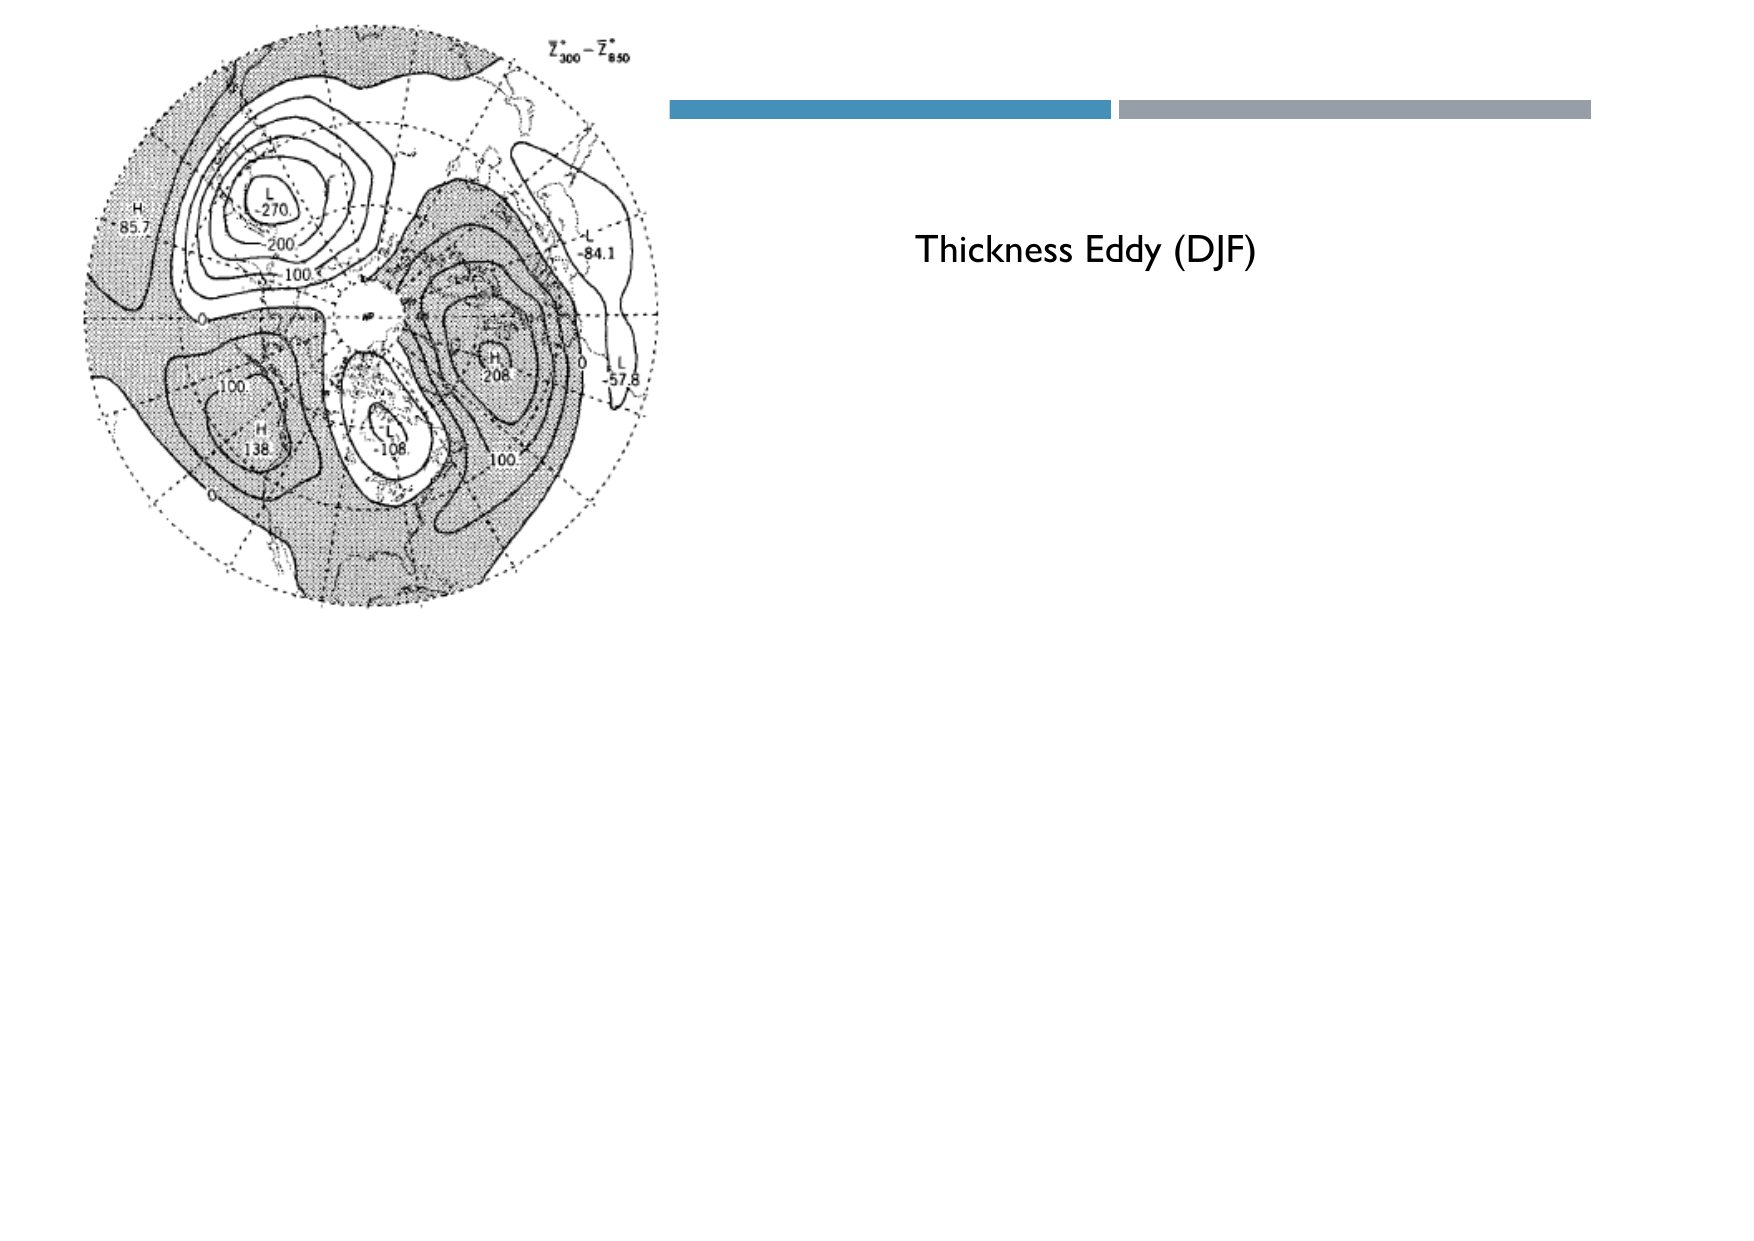
\includegraphics[width=0.85\textwidth]{images/ch06/p35_img01.png}
  \caption{Time-mean thickness eddy field $Z_E$ between 1000 and 500\,hPa
    for DJF (Lau, 1979).  Shaded high over central Asia (Tibetan Plateau region)
    and low centres over eastern North America and the North Atlantic
    delineate the planetary-scale zonally asymmetric component of the
    mid-troposphere.
    \hisu{1000--500\,hPa 두께장의 eddy 성분 (DJF).
          중앙아시아의 양의 thickness 이상과 북미 동부/북대서양의 음의 이상이
          행성 규모 stationary wave의 본체이다.}}
  \label{fig:ch06_sw_thickness_djf}
\end{figure}

Thickness $Z(1000\text{-}500)$는 1000--500 hPa 층의 \emph{평균 온도}에 비례한다
(hypsometric equation, Ch.3).
따라서 그림 \ref{fig:ch06_sw_thickness_djf}의 양의 thickness 이상은
대류권 중층까지의 \emph{평균 온도가 zonal mean보다 높은} 지역을,
음의 이상은 반대 지역을 나타낸다.
중앙아시아 위 양의 anomaly는 Tibetan Plateau의 상승된 지표면에서의
sensible heating, 북미 동부의 음의 anomaly는 강한 long-wave cooling 영향이 결합된 결과다.

\medskip



\noindent\textbf{Geopotential height eddy $Z_E$: latitudinal cross-sections.}

\begin{figure}[htbp]
  \centering
  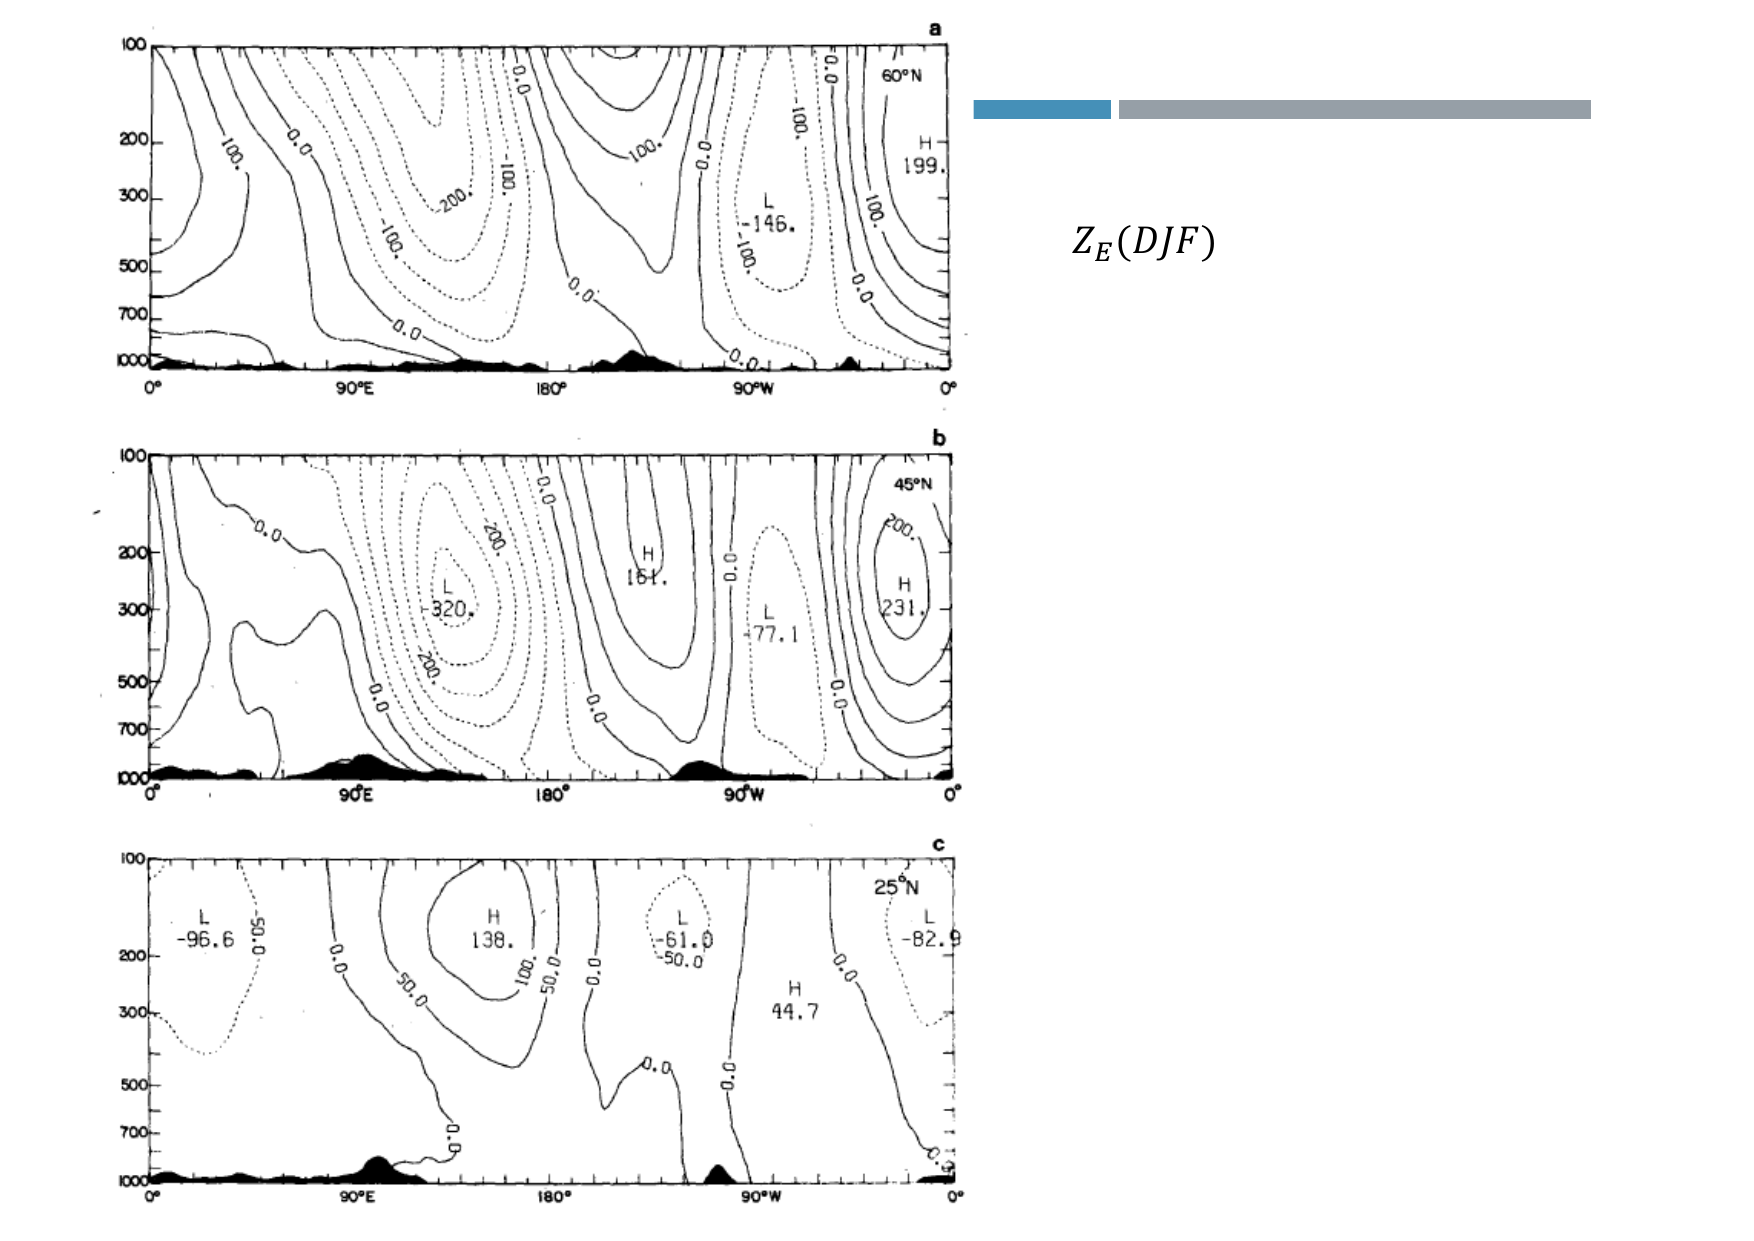
\includegraphics[width=0.85\textwidth]{images/ch06/p36_img01.png}
  \caption{Longitude--pressure cross-sections of the geopotential height eddy
    $Z_E$ for DJF at (top)~$60^\circ$N, (middle)~$45^\circ$N, and (bottom)~$25^\circ$N.
    Solid (dashed) contours denote positive (negative) anomalies.  At $60^\circ$N,
    the largest negative $Z_E$ (around $-193$\,m) appears in the upper troposphere
    near 200\,hPa over the North Pacific; at $45^\circ$N the amplitude is moderated
    (extremes near $+231$\,m and $-177$\,m); at $25^\circ$N the eddy is shallow
    and weak.
    \hisu{고도별 stationary wave 단면.  60$^\circ$N에서 상층 음의 이상이 매우 강하고,
          45$^\circ$N에서 진폭은 중간이지만 mid-troposphere까지 깊게 연장,
          25$^\circ$N에서는 진폭이 작고 phase 구조만 남는다.}}
  \label{fig:ch06_sw_zecross}
\end{figure}

그림 \ref{fig:ch06_sw_zecross}에서 가장 주목할 특징은 \emph{vertical alignment}이다.
$60^\circ$N과 $45^\circ$N 모두에서 $Z_E$ 등치선이 거의 수직, 즉 troposphere 전체에 걸쳐
같은 부호의 이상이 정렬되어 있다.
이것이 \textgr{barotropic} 수직 구조를 의미하며, 발달 단계의 transient eddy가 갖는
westward tilt(Ch.5)와 대비된다.
즉 stationary wave는 \emph{이미 성숙한, 베어보트로픽한 구조}로 평균 상태에 자리 잡고 있다.

\medskip



\noindent\textbf{Temperature eddy $T_E$: latitudinal cross-sections.}

\begin{figure}[htbp]
  \centering
  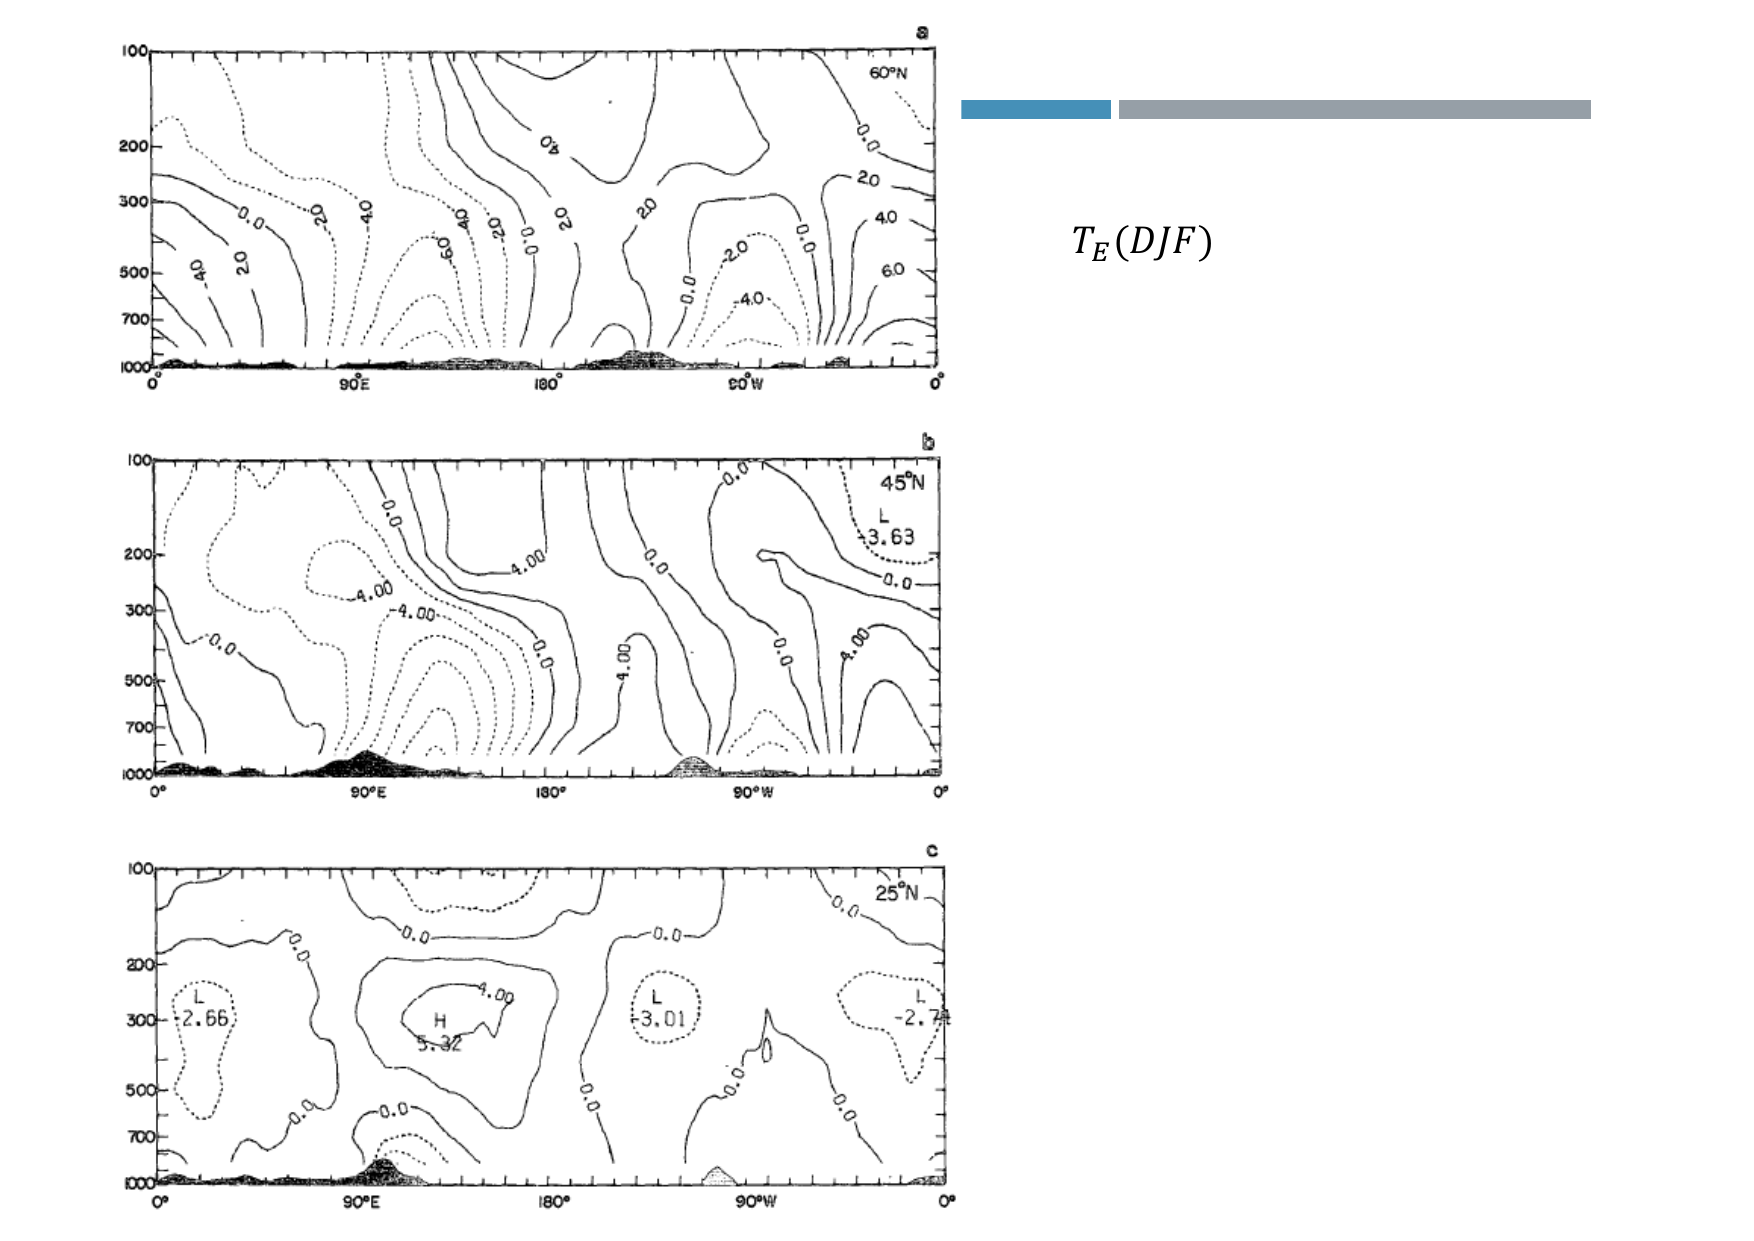
\includegraphics[width=0.85\textwidth]{images/ch06/p37_img01.png}
  \caption{Same as Fig.~\ref{fig:ch06_sw_zecross} but for the temperature eddy
    $T_E$.  Below $\sim 500$\,hPa, $T_E$ tends to be \emph{out of phase}
    with $Z_E$ (cold over the low, warm over the high) in mid-latitudes,
    consistent with the lower-tropospheric thermal forcing.  Above
    $\sim 300$\,hPa, the sign flips, reflecting the stratosphere--troposphere
    transition.
    \hisu{온도 이상 단면.  하층에서 $Z_E$와 위상이 반대 (저기압 위가 차고 고기압 위가 따뜻함),
          상층에서 부호 반전 — diabatic forcing의 흔적.}}
  \label{fig:ch06_sw_tecross}
\end{figure}

그림 \ref{fig:ch06_sw_zecross}와 \ref{fig:ch06_sw_tecross}을 결합하면
hypsometric eq.\ $\partial Z_E/\partial p = -RT_E/(gp)$ 와 일관된 결과가 얻어진다.
\textbf{Continental cold lows}(Siberia, Canada)는 lower troposphere의 $T_E < 0$와
upper troposphere의 $Z_E < 0$가 연직 정렬된 결과이다.

\medskip



\noindent\textbf{Momentum flux convergence.}

\begin{figure}[htbp]
  \centering
  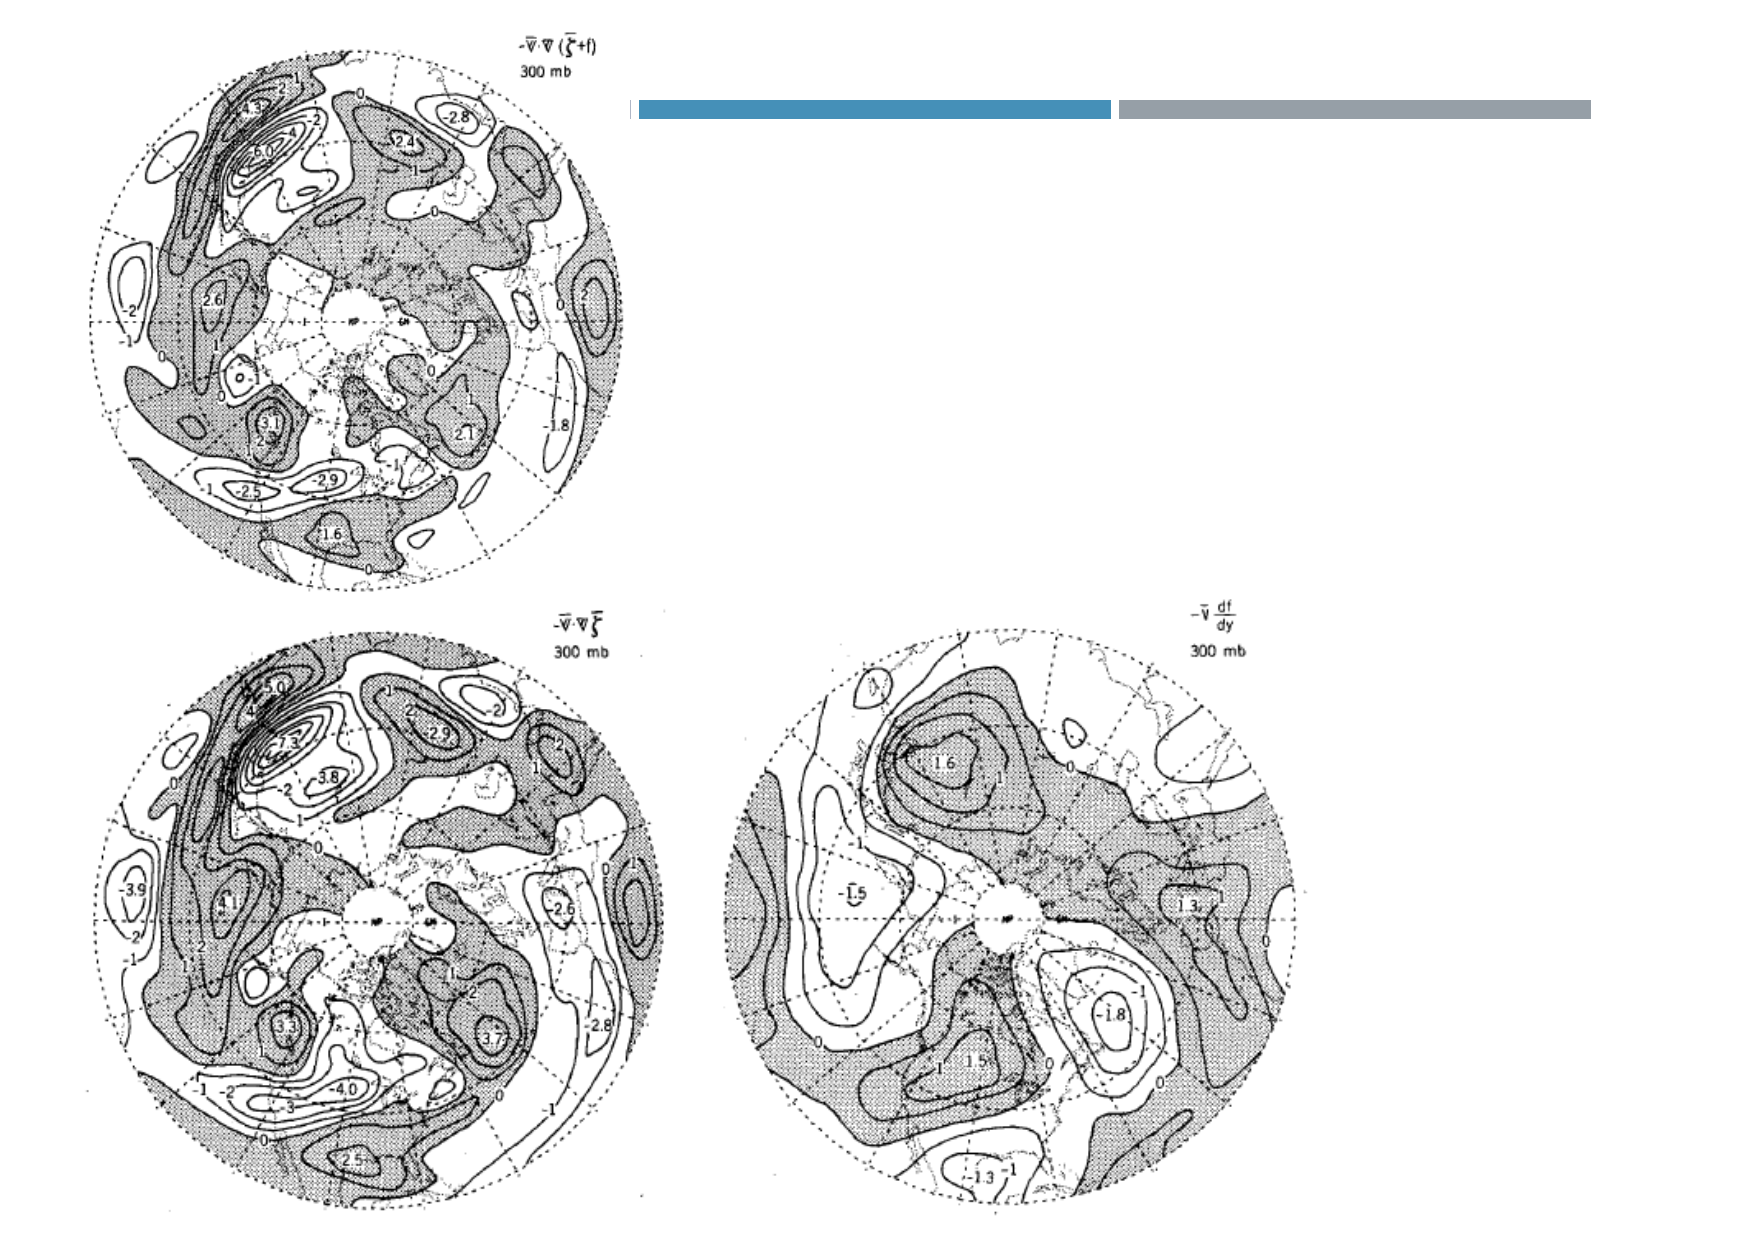
\includegraphics[width=0.85\textwidth]{images/ch06/p38_img01.png}
  \caption{Time-mean negative meridional momentum flux $-\overline{V'u'}$
    at 300\,hPa for DJF (four-panel by season/component).
    Positive values indicate poleward transport of westerly momentum.
    Maxima are anchored over the western Pacific and western Atlantic
    storm-track exit regions, consistent with the location of the
    upper-tropospheric jet maxima.
    \hisu{상층 momentum flux: storm track 출구 부근에서 최대 poleward westerly 수송.
          여기가 곧 jet stream을 유지하는 핵심 영역.}}
  \label{fig:ch06_sw_momflux}
\end{figure}

$-\overline{V'u'} > 0$는 westerly momentum의 \emph{poleward transport}를 뜻한다.
북반구 중위도에서 이 값은 storm track 출구 부근에서 양으로 최대가 되는데,
이는 §1에서 본 ageostrophic wind 분석과 일관된다:
jet exit에서 ageostrophic 남풍이 westerly 운동량을 북쪽으로 운반한다.
이 momentum flux의 \emph{convergence}가 곧 평균 jet의 \emph{유지} 메커니즘이다.

\medskip



\noindent\textbf{Heat flux at the lower troposphere.}

\begin{figure}[htbp]
  \centering
  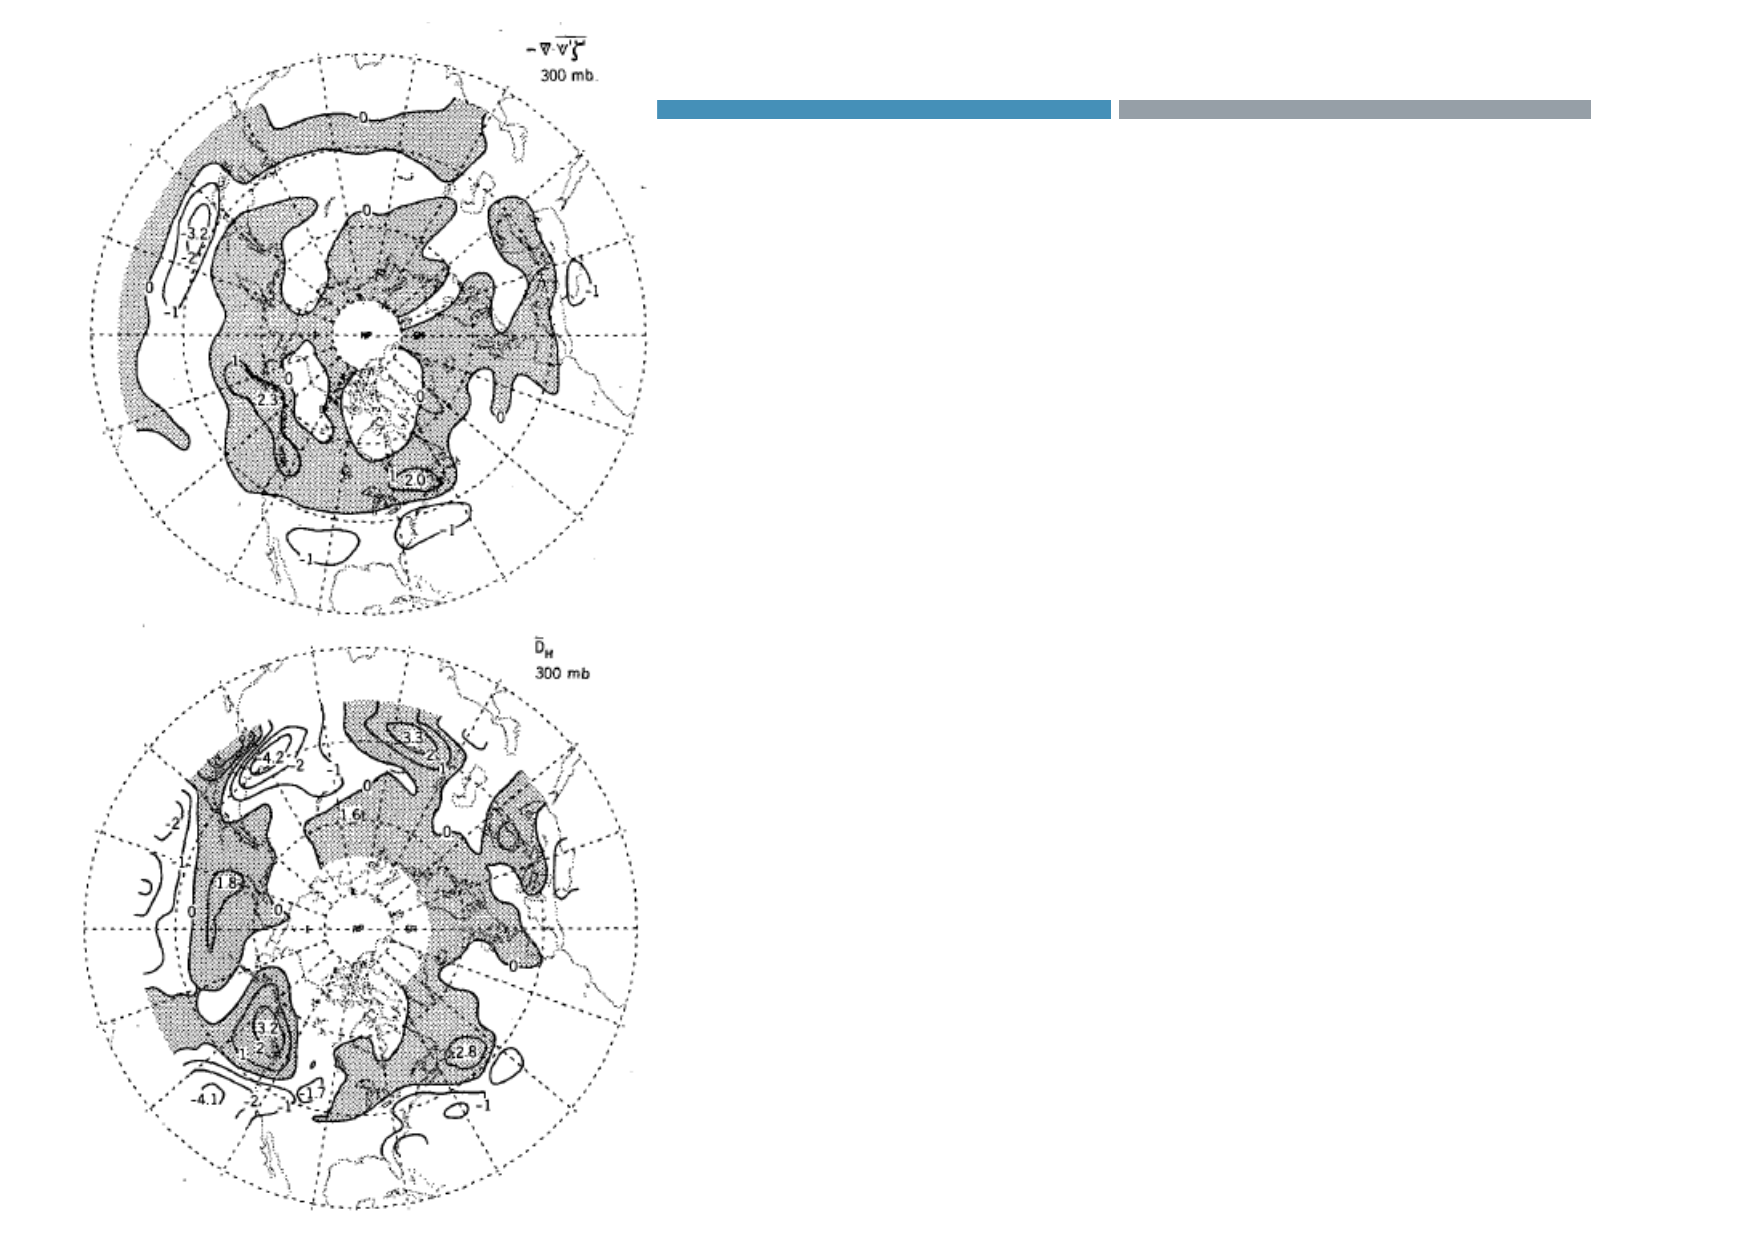
\includegraphics[width=0.85\textwidth]{images/ch06/p39_img01.png}
  \caption{Poleward eddy heat flux $\overline{v'T'}$ at 1000\,hPa for DJF
    (four-panel).  Positive maxima over the western boundary current regions
    (Kuroshio, Gulf Stream) indicate strong low-level heat transport by
    cyclones during their early development, where warm marine air is advected
    poleward ahead of the cold front.
    \hisu{지표 부근의 자오 열수송.  Kuroshio와 Gulf Stream 위에서 최대 — 해양에서
          공급된 따뜻한 공기가 cyclone 동측을 따라 극지로 운반된다.}}
  \label{fig:ch06_sw_heatflux1000}
\end{figure}

$\overline{v'T'}$의 양의 극값이 western boundary current 위에 위치한다는 사실은
\textbf{baroclinic instability}의 지리적 사인이다.
강한 SST gradient는 강한 lower-tropospheric baroclinicity를 만들고,
그 위에서 가장 활발한 transient eddy 성장이 일어난다.
이 heat flux의 convergence가 \eqref{eq:ch06_sw_heatfull}의 둘째 항을 통해
극지방의 stationary cold low 유지에 기여한다.

\medskip



\noindent\textbf{Multi-field composites: upper and lower troposphere.}

\begin{figure}[htbp]
  \centering
  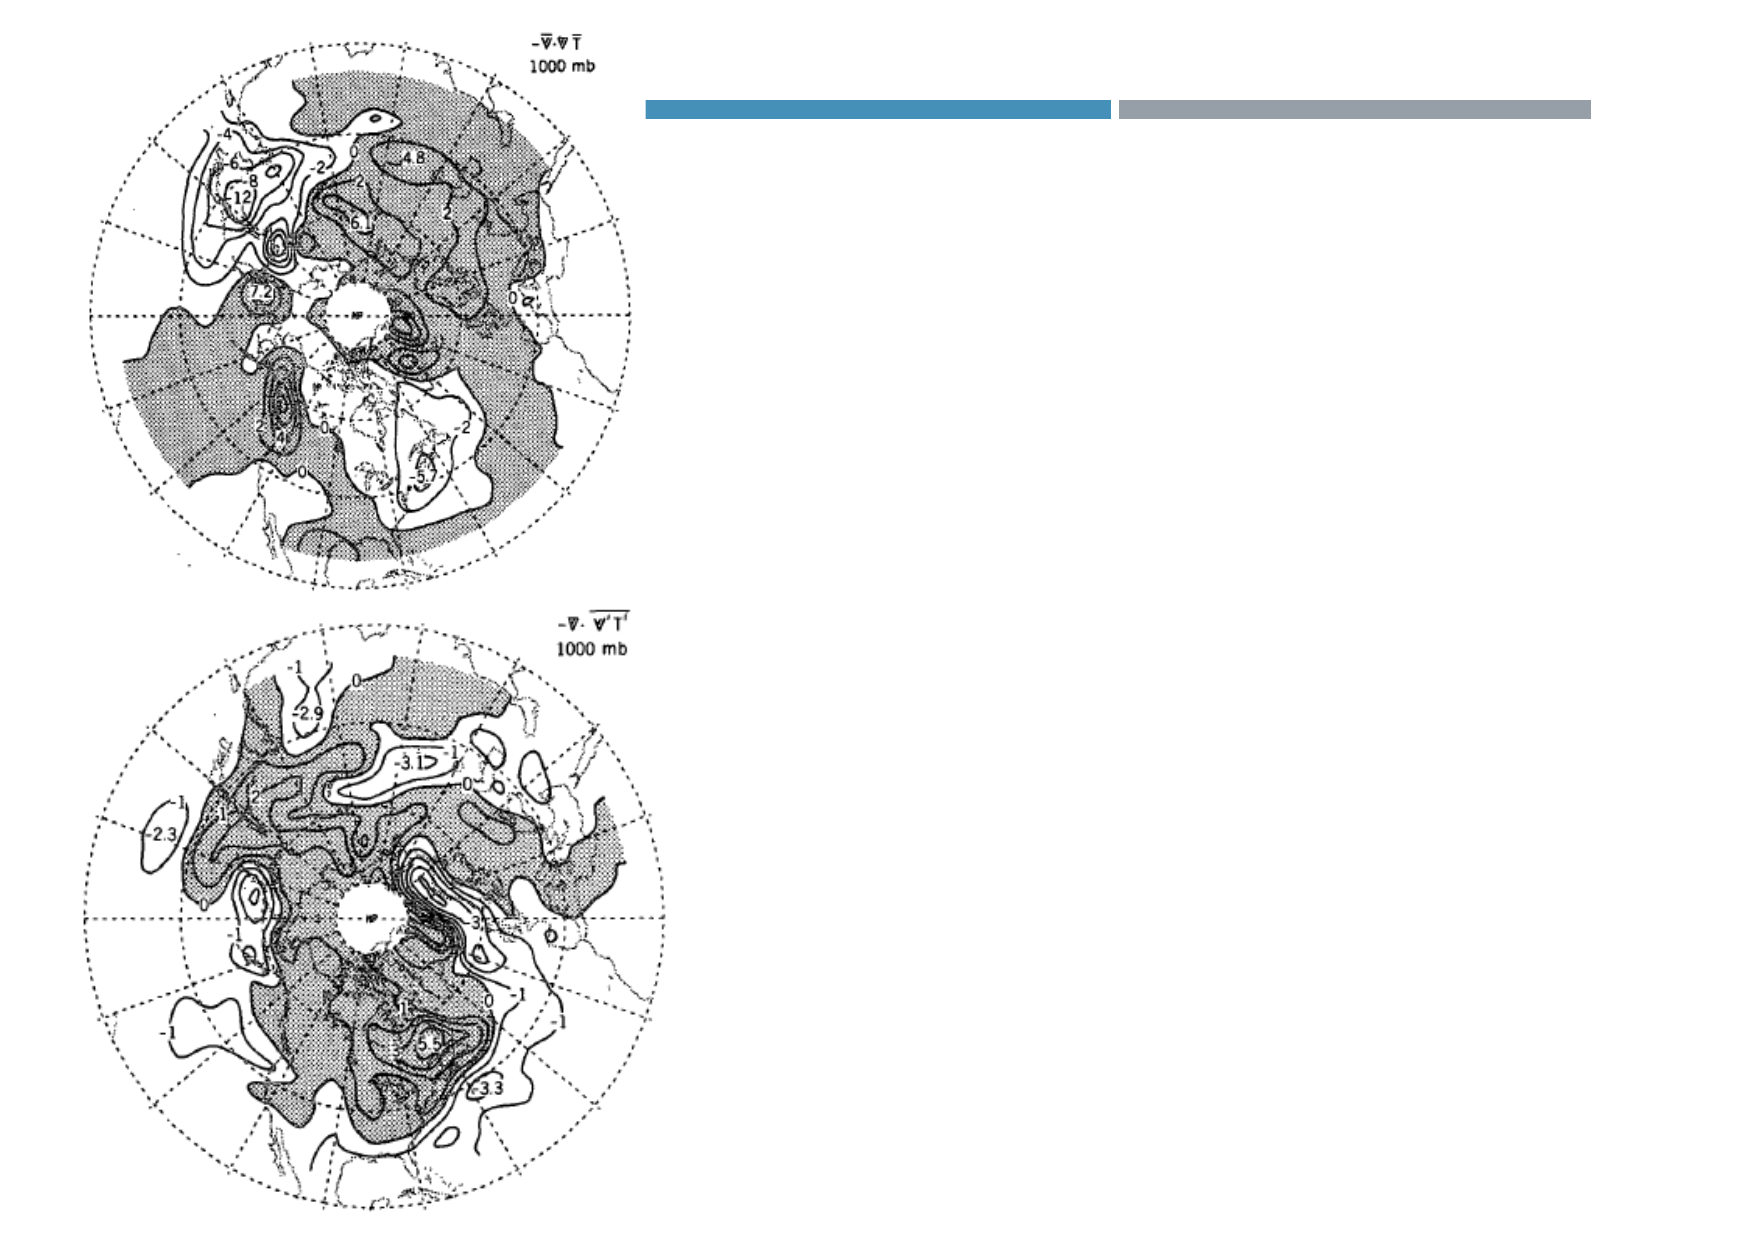
\includegraphics[width=0.85\textwidth]{images/ch06/p40_img01.png}
  \caption{Multi-field composites for DJF showing eddy fields at 300\,hPa
    (upper troposphere) and 1000\,hPa (lower troposphere) superposed.
    The displacement between the upper geopotential ridge/trough and the
    lower-tropospheric heat-flux/vorticity centres provides direct
    observational evidence for the quarter-phase shift between rotational
    and divergent components (Theorem~\ref{thm:ch06_sw_qps}).
    \hisu{상하층 다층 합성 — 상층 ridge/trough와 하층 vorticity/heat 패턴 사이의
          어긋남은 \ref{thm:ch06_sw_qps} 정리의 관측적 확인이다.}}
  \label{fig:ch06_sw_composites}
\end{figure}

이 그림은 본 절의 \emph{최종 종합도}로 읽혀야 한다.
상층 ridge ($Z_E > 0$의 중심)와 그 아래 lower-troposphere heat flux 극값,
그리고 surface vorticity 패턴이 \emph{경도 방향으로} 한 분의 1 파장만큼 어긋난 위치에 자리한 모습이
quarter-phase shift theorem \eqref{eq:ch06_sw_qps}의 관측적 검증이다.

\medskip



\noindent\textbf{Surface vorticity.}

\begin{figure}[htbp]
  \centering
  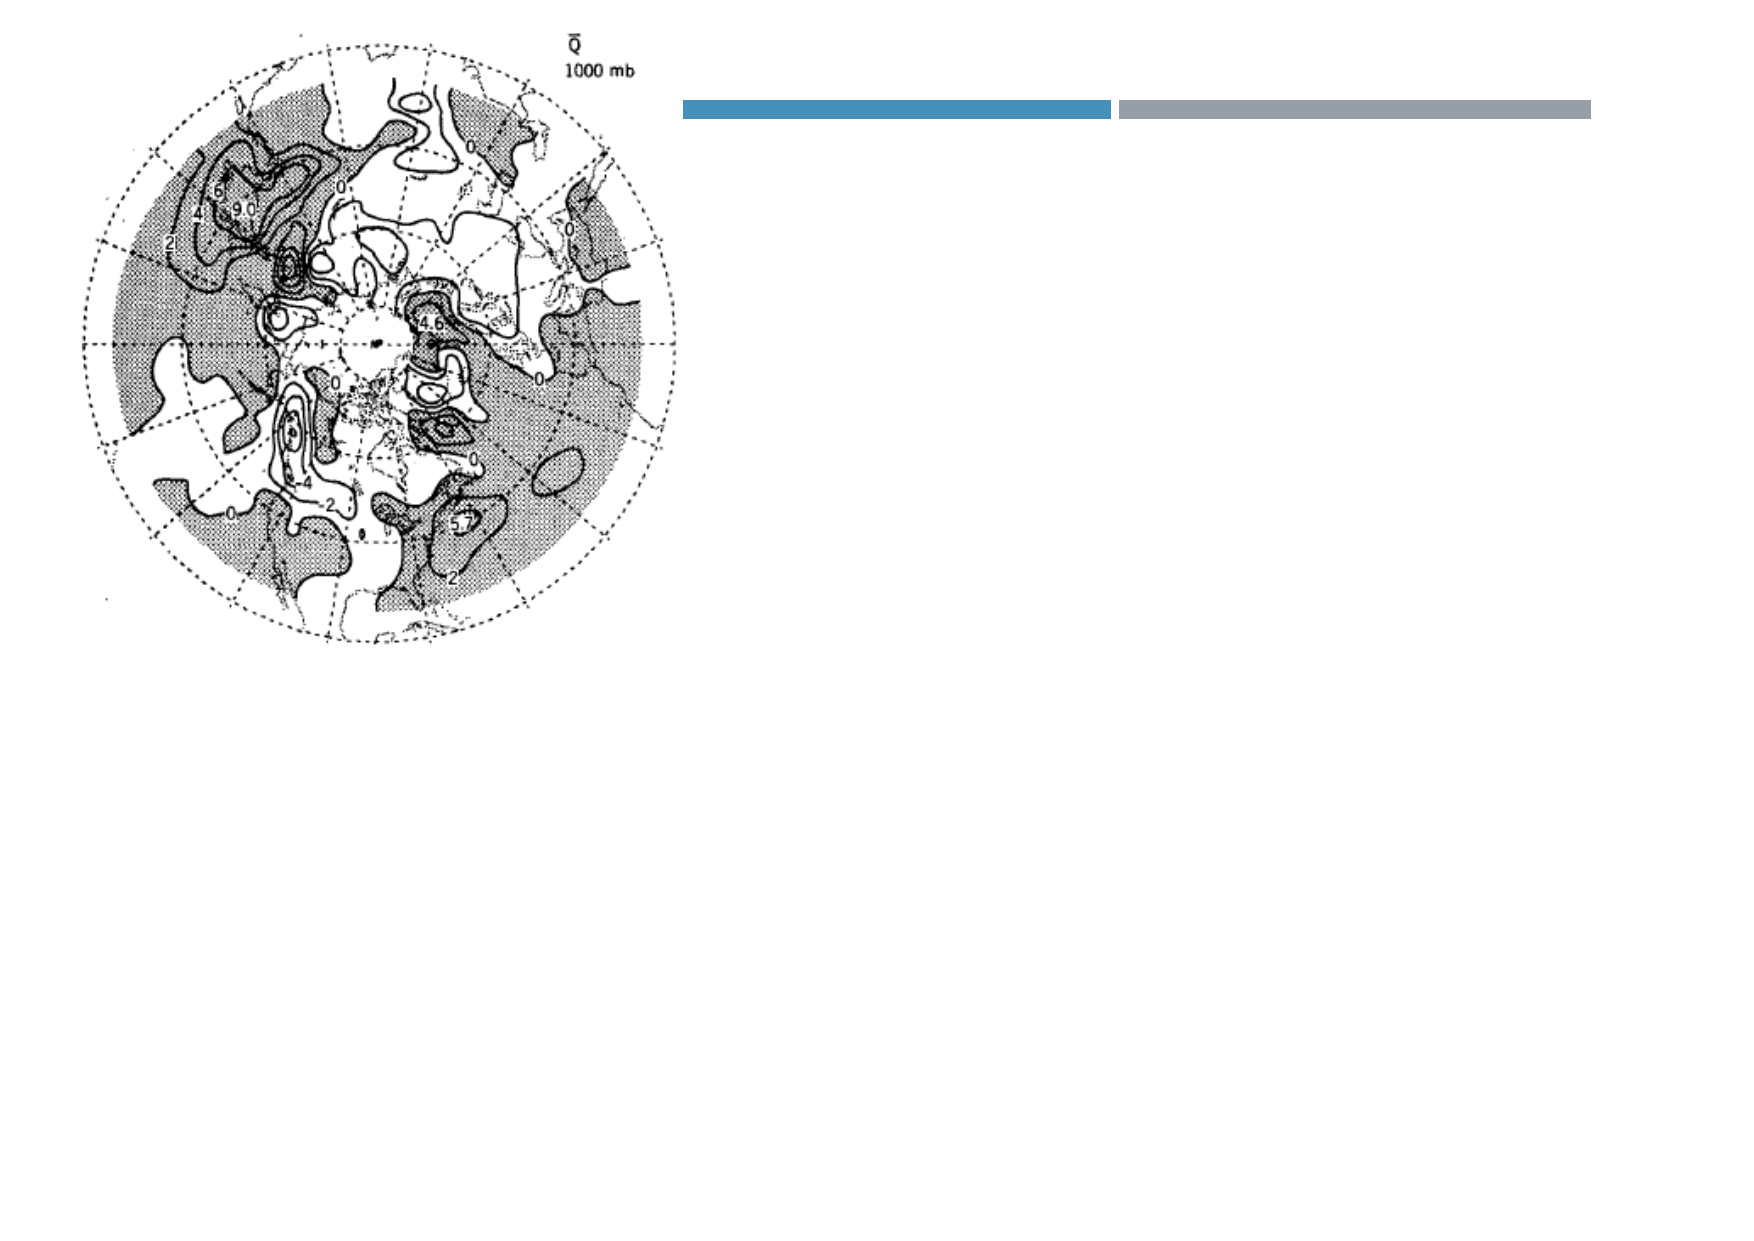
\includegraphics[width=0.85\textwidth]{images/ch06/p41_img01.png}
  \caption{Time-mean surface relative vorticity $\overline{\xi}$ at 1000\,hPa
    for DJF.  Cyclonic (positive) maxima over the Aleutian Low region and the
    Icelandic Low region, anticyclonic (negative) maxima over the Siberian
    High and the subtropical highs.  These surface vorticity centres are
    the \emph{stationary footprints} of the planetary wave pattern shown
    above, and through Ekman pumping (Eq.~\ref{eq:ch06_sw_omegaF}) they
    feed back to the free-tropospheric vertical motion.
    \hisu{지표 평균 vorticity.  Aleutian/Icelandic low의 양의 vorticity,
          Siberian high의 음의 vorticity가 stationary wave의 ``발자국''.
          Ekman pumping을 통해 자유 대기 $\overline{\omega}$의 하부 경계 조건이 된다.}}
  \label{fig:ch06_sw_xi1000}
\end{figure}

\begin{remark}[Closing the Loop]\label{rem:ch06_sw_closure}
그림 \ref{fig:ch06_sw_xi1000}은 본 절 전체를 \emph{닫아 준다}.
이 surface vorticity field가 \eqref{eq:ch06_sw_omegaF}을 통해 $\overline{\omega}_F$를 결정하고,
\eqref{eq:ch06_sw_omega_integral}을 통해 모든 고도의 $\overline{\omega}$의 출발점이 된다.
그리고 $\overline{\omega}$는 다시 vorticity stretching $(f+\overline{\zeta})\nabla\!\cdot\!\overline{\mathbf{V}}$를 통해
\eqref{eq:ch06_sw_vorbal_final}의 vorticity 균형을 닫는다.
즉 \textbf{stationary wave는 표면 vorticity로부터 출발해 다시 표면으로 돌아오는 닫힌 회로}이다.
\end{remark}

\hisu{지표 vorticity → Ekman pumping → 자유 대기 $\overline{\omega}$ → vortex stretching → 다시 지표 vorticity. 이 닫힌 회로가 stationary wave 유지의 본질.}

% --------------------------------------------------------------------------
\subsubsection*{Section Summary}
% --------------------------------------------------------------------------

\begin{remarkbox}
본 절 (§3)의 다섯 가지 핵심 메시지는 다음과 같다.
\begin{enumerate}
  \item \textbf{Stationary eddies dominate local maintenance}:
        시간 분산은 transient eddies가 지배하지만, 운동량·열·운동에너지의 \emph{지역적} 평균을
        유지하는 데에는 stationary eddies가 결정적이다 (Remark~\ref{rem:ch06_sw_brake}).
  \item \textbf{Transient vorticity flux convergence는 jet에 brake}:
        $-\nabla\!\cdot\!\overline{\mathbf{V}'\zeta'}$이 평균 jet을 감속시킨다 (\eqref{eq:ch06_sw_vorbal_final}).
  \item \textbf{Mountain torque vs.\ friction이 vertical motion의 lower BC}:
        $\overline{\omega}_M$과 $\overline{\omega}_F$ 두 항이 자유 대기 평균 vertical motion의 출발점을 결정한다
        (\eqref{eq:ch06_sw_omegaM}--\eqref{eq:ch06_sw_omegaF}).
  \item \textbf{Rotational/divergent 분해가 vorticity source를 분리}:
        $\overline{\mathbf{V}} = \overline{\mathbf{V}}_R + \overline{\mathbf{V}}_D$로 가르면 RWS \eqref{eq:ch06_sw_RWS}이
        깔끔히 떨어져 나오며, 이는 teleconnection 이론의 기초가 된다.
  \item \textbf{$\Psi$--$\chi$ Quarter-Phase Shift}:
        Theorem~\ref{thm:ch06_sw_qps}에 따라 streamfunction과 velocity potential은 $90^\circ$
        어긋나 있다.  이것이 stationary wave 3차원 구조의 기본 골격이며, Lau (1979)의 관측이
        이를 확증한다 (Fig.~\ref{fig:ch06_sw_composites}).
\end{enumerate}
\end{remarkbox}

\begin{hisublock}
\textbf{한국어 종합 정리}.
\begin{enumerate}
  \item Stationary wave는 변동 분산이 아니라 \emph{지역적 평균값}을 유지하는 주역이다.
  \item Transient eddy의 vorticity flux는 평균 jet을 가속하지 않고 \emph{감속}시킨다.
  \item 지표의 산악 끌어올림과 Ekman pumping이 \emph{자유 대기 $\overline{\omega}$의 하부 경계}를 결정.
  \item 회전·발산 분해가 \emph{Rossby wave source}(RWS)를 정의하고, 이는 열대-중위도 텔레커넥션의 다리.
  \item Streamfunction과 velocity potential의 $90^\circ$ 어긋남은 stationary wave의 \emph{생긴 모양}을 한 줄로 요약한다.
\end{enumerate}

\medskip
\textbf{다음 절(§4)로의 연결}: 본 절에서 인용한 다섯 편의 핵심 논문
(Blackmon et al.\ 1977; Held 1983; Lau 1979a, 1979b; Chen et al.\ 2005)을
§4 References Deep Dive에서 식·그림 수준으로 정밀하게 비교한다.
\end{hisublock}
% =============================================================================
%   SECTION 4 — References Deep Dive
% =============================================================================

\subsection{References Deep Dive}

본 챕터의 본문은 NH 겨울 순환의 \textgr{stationary}와 \textgr{transient} 성분이
각각 어디에 어떤 구조로 존재하고, 무엇이 그것을 유지하는지를 다루었다.
그러나 본문에서 인용한 모든 figure --- variance map, vertical cross-section,
eddy flux composite, 지형 강제 응답 --- 의 원 출처를 한자리에 모아두면
독자가 자신의 분석을 시작할 때 어떤 논문을 가장 먼저 펼쳐야 하는지 분명해진다.
이 절은 그러한 안내를 위해 다섯 편의 논문을 정밀하게 정리한다.

다섯 편은 \emph{어디(where)} -- \emph{왜 거기(why)} -- \emph{어떤 vertical 구조(how, vertically)} --
\emph{어떤 balance로 유지(how, balanced)} -- \emph{tropics extension} 의 다섯 질문에
한 편씩 대응한다.  \textbf{Blackmon \emph{et al.} (1977)}은 시간 필터링과 분산 분해로
지리적 분포를 처음 체계화했고, \textbf{Held (1983)}은 그 패턴이 왜 그 위치에 자리잡는지를
정상파 이론으로 답했다.  \textbf{Lau (1979a)}는 transient eddy의 수직 에너지 변환 경로를
정량화했으며, \textbf{Lau (1979b)}는 stationary wave를 vorticity와 heat balance로 풀어냈다.
끝으로 \textbf{Chen \emph{et al.} (2005)}은 동일한 분해 framework가 열대 monsoon
저기압의 서진(westward propagation)에도 적용됨을 보였다.

\hisu{이 다섯 편을 한 줄로 묶으면: ``어디 + 왜 + 어떻게 vertically + 어떻게 balanced + tropics까지.''}


% --------------------------------------------------------------------------
\subsubsection{Blackmon \emph{et al.} (1977): Band-Pass Decomposition of NH Winter Circulation}

\textbf{Blackmon, M.~L., Wallace, J.~M., Lau, N.-C., and Mullen, S.~L., 1977:
An observational study of the Northern Hemisphere wintertime circulation.
\emph{J.\ Atmos.\ Sci.}, \textbf{34}, 1040--1053.}

\medskip
\noindent\textbf{Motivation.}\quad
1970년대 중반까지 북반구 겨울 대순환에 대한 분석은 양극단 사이를 오가고 있었다.
한쪽에는 세 달 평균(DJF climatology)을 다루는 연구가 있었고 --- 이 경우 transient
정보가 모두 평균에 흡수되어 storm track의 존재 자체가 보이지 않는다 --- 다른 한쪽에는
개별 사이클론 사례 연구가 있었으나 통계적으로 어디에서 ``평균적으로''
transient activity가 가장 강한지를 객관적으로 답하지 못했다.
본 논문은 두 접근 사이의 빈 칸을 채우기 위해, 일별(daily) 자료에 \textgr{band-pass filter}를
체계적으로 적용해 시간 척도별로 분산을 분해하는 방법을 처음 정립했다.

\medskip
\noindent\textbf{Data \& Method.}\quad
자료는 1965--1976년 11겨울의 500~mb 지위고도 daily field, 2.5$^\circ\times$2.5$^\circ$ grid이다.
시간 분해는 세 채널로 이루어진다:
\begin{equation}\label{eq:ch06_dd_blackmon_filter}
  h(\mathbf{x},t) \;=\; h_{\mathrm{LP}}(\mathbf{x},t)
  \;+\; h_{\mathrm{BP}}(\mathbf{x},t)
  \;+\; h_{\mathrm{HP}}(\mathbf{x},t),
\end{equation}
여기서 LP는 $T>90$~days (stationary wave + low-frequency teleconnection),
BP는 $2.5\le T\le 6$~days (\textgr{baroclinic transient eddies}, 즉 storm track),
HP는 $T<2.5$~days (high-frequency noise + small-scale wave)이다.
세 성분은 서로 통계적으로 거의 독립이므로 분산 분해
\begin{equation}\label{eq:ch06_dd_blackmon_variance}
  \sigma^2_{\text{total}}
  \;=\; \sigma^2_{\mathrm{LP}}
  + \sigma^2_{\mathrm{BP}}
  + \sigma^2_{\mathrm{HP}}
\end{equation}
가 성립한다.  Heat transport와 같은 2차 통계량은
$\overline{v'T'} = n^{-1}\sum_i v'_i T'_i$로 daily anomaly product를 평균하여 얻는다.

\medskip
\noindent\textbf{Key Results.}
\begin{itemize}
  \item Total $\sigma^2$의 최대치는 35--55$^\circ$N의 좁은 띠를 따라 나타나며,
        이는 곧 \textgr{storm track}의 객관적 정의가 된다.
  \item Band-pass 성분은 고위도(50$^\circ$N 이북)에서 전체 분산의 60--80\%를 차지하나,
        아열대(35$^\circ$N 이남)에서는 standing/LP 성분이 우세하다.
  \item Pacific storm track은 150$^\circ$E--120$^\circ$W의 40--50$^\circ$N 위도대에,
        Atlantic storm track은 60$^\circ$W--20$^\circ$W의 45--55$^\circ$N 위도대에
        뚜렷이 자리한다 --- 두 jet exit region과 거의 일치.
  \item Band-pass $\overline{v'T'}$의 최대값은 850~mb 부근에서 10--15~K~m/s,
        30$^\circ$N 이북에서 mean meridional circulation의 열 수송을 능가한다.
  \item Standing wave의 진폭은 60$^\circ$N에서 500~mb 지위고도 $\pm$150~m,
        transient envelope보다 큰 평균 신호를 만든다.
\end{itemize}

\medskip
\noindent\textbf{Connection to Ch.~6.}\quad
본 챕터 \S1의 ``Storm Tracks and Variance Maps'' figure는 직접적으로 이 논문 Fig.~2--5에서
가져온 것이며, 본문 \S1.2에서 도입한 시간 필터링 \eqref{eq:ch06_dd_blackmon_filter}의 정의가
바로 Blackmon \emph{et al.}\ 의 분류에 따른 것이다.  또한 \S1.3 ``Eddy heat flux maps''의
850~mb $\overline{v'T'}$ composite도 본 논문의 결과를 reanalysis-era 자료로 재현한 것이다.

\begin{hisublock}
이 논문을 다음과 같이 활용하라:
\begin{itemize}
  \item 본 챕터 \S1.1의 figure는 이 논문 Fig.~2의 quantity와 동일하다 ---
        500~mb 지위고도의 LP/BP 분산 분포를 비교할 때 직접 참조.
  \item 본문 \eqref{eq:ch06_dd_blackmon_filter}--\eqref{eq:ch06_dd_blackmon_variance}는
        Holton \& Hakim Ch.~10 ``Mean Flow--Eddy Interaction''의 시간 평균 분해를
        \emph{daily-scale filter}로 일반화한 것이다.
  \item Storm track의 객관적 정의(BP variance maximum)는 본 책의 \S2와 \S3에서
        ``transient eddy structure''와 ``stationary structure'' 의 분리 기준이 된다.
  \item 한계: 본 논문은 500~mb 단일 level만 본다. Vertical structure는
        Lau (1979a)에서 보완되며 본 책 \S2가 그것을 다룬다.
\end{itemize}
\end{hisublock}


% --------------------------------------------------------------------------
\subsubsection{Held (1983): Theory of Stationary Waves}

\textbf{Held, I.~M., 1983: Stationary and quasi-stationary eddies in the extratropical troposphere: Theory.
In: B.~Saltzman (Ed.), \emph{Large-Scale Dynamical Processes in the Atmosphere},
Academic Press, Chapter~6, pp.~127--168.}

\medskip
\noindent\textbf{Motivation.}\quad
Blackmon \emph{et al.}\ (1977)이 standing wave가 ``어디에'' 있는지를 보였다면,
Held는 ``\emph{왜} 거기에'' 있는지를 묻는다.  관측된 NH 겨울 stationary pattern ---
북미 동부의 trough, 동대서양/서유럽의 ridge, 동아시아 trough ---
는 mean zonal wind $\bar u$의 강도와 어떻게 관계되는가?
그리고 Rocky Mountain과 Tibetan Plateau 같은 지형은 정량적으로 얼마나 기여하는가?
Held는 \textgr{stationary Rossby wave} 이론을 framework로 삼아 이 질문을
이론적으로 해부한다.

\medskip
\noindent\textbf{Data \& Method.}\quad
본 논문은 관측 자료에 의존하지 않는 이론적 chapter이다.  출발점은 베타 평면에서의
선형화된 \textgr{quasi-geostrophic vorticity equation}
\begin{equation}\label{eq:ch06_dd_held_qg}
  \pdt{\nabla^2\psi'} \;+\; \bar u\,\pdx{\nabla^2\psi'}
  \;+\; \beta\,\pdx{\psi'} \;=\; F(x,y),
\end{equation}
여기서 $F$는 지형 강제 $\bar u (f/H)\nabla h_{\text{topo}}$ 또는 diabatic vorticity source.
파동해 $\psi' = \hat\psi(y)\,e^{i(kx-\omega t)}$를 대입하면 분산 관계
\begin{equation}\label{eq:ch06_dd_held_dispersion}
  \omega \;=\; \bar u k \;-\; \frac{\beta\,k}{k^2 + l^2}
\end{equation}
가 나오고, \emph{stationary} 조건 $\omega = 0$은
\begin{equation}\label{eq:ch06_dd_held_resonant_k}
  \boxed{\;k_s^2 + l^2 \;=\; \frac{\beta}{\bar u}\;}
\end{equation}
의 \textgr{stationary wavenumber}를 정의한다.  지형 강제에 대한 정상상태 응답은
\begin{equation}\label{eq:ch06_dd_held_topo_response}
  \hat\psi_{\text{topo}}
  \;\propto\; \frac{f h_0 / H}{k^2 - k_s^2},
\end{equation}
이므로 $k\to k_s$에서 응답이 발산(resonance)한다.  Held는 베타 평면 분석에 이어
구면(sphere) 모델로 확장하고, 실제 지형과 diabatic forcing을 함께 부과해 응답 패턴을 그린다.

\medskip
\noindent\textbf{Key Results.}
\begin{itemize}
  \item Mean wind $\bar u$가 약해질수록 $k_s$가 작아져 stationary response 진폭이
        증가한다(공명에 접근).
  \item 실제 지형만으로 강제된 spherical 모델 응답은 관측된 NH winter
        standing pattern을 정성적으로 재현하며, 진폭의 50--70\%를 설명한다.
  \item Rocky Mountain은 가장 강한 강제원이고, Tibetan Plateau는 그 다음.
        두 산맥 모두 그 동쪽에 trough를 만든다 --- ``downstream trough'' 규칙.
  \item Diabatic forcing(특히 storm track 가열, ocean western boundary current)을
        추가하면 진폭이 70--90\%로 향상.
  \item 평균풍 약화 시 stationary pattern이 polewards로 이동 ---
        과거 빙기 climate state에서의 jet 이동 해석에 유용.
\end{itemize}

\medskip
\noindent\textbf{Connection to Ch.~6.}\quad
본 챕터 \S3.1 ``Stationary Wave Theory''의 모든 식 ---
linear vorticity equation, dispersion relation, stationary wavenumber $k_s = \sqrt{\beta/\bar u}$ ---
은 Held (1983)의 베타 평면 정식화를 그대로 따른 것이다.  본문에서
``mountain forcing'' 과 ``diabatic forcing'' 을 두 강제 메커니즘으로 구분한 것도 이 논문 분류이다.

\begin{hisublock}
이 논문을 다음과 같이 활용하라:
\begin{itemize}
  \item 본 챕터 \S3.1에서 도입한 $k_s^2 = \beta/\bar u$
        \eqref{eq:ch06_dd_held_resonant_k}는 Held (1983) Eq.~(3.4)와 동일한 식이다.
  \item ``왜 trough가 산맥 \emph{동쪽}에 있는가?'' 는 본 책 \S3.2 figure(지형 강제 응답)
        해설에서 직접 이 논문 Fig.~6.2의 mountain-forced response를 참고한다.
  \item Linear barotropic 가정의 한계 --- vertical propagation, baroclinic 효과 무시 ---
        는 Charney--Drazin(본 책 \S4에서 인용)와 함께 읽어야 한다.
  \item 본 책 \S3.3 ``Maintenance Mechanism'' 에서 ``stationary wave는 locally
        forced + globally dispersed'' 라고 적은 결론은 이 논문의 메시지이다.
\end{itemize}
\end{hisublock}


% --------------------------------------------------------------------------
\subsubsection{Lau (1979a): Vertical Energetics of Transient Disturbances}

\textbf{Lau, N.-C., 1979: The structure and energetics of transient disturbances in the Northern Hemisphere wintertime circulation.
\emph{J.\ Atmos.\ Sci.}, \textbf{36}, 982--995.  [Lau~1979a]}

\medskip
\noindent\textbf{Motivation.}\quad
Blackmon \emph{et al.}\ (1977)이 BP transient의 \emph{수평} 분포(storm track의 위치)는
규명했으나, transient eddy가 \emph{수직적으로} 어떻게 조직되고 어디에서 에너지를
획득하는지는 미해결로 남아 있었다.  특히 transient의 baroclinic structure --- 위상이 고도에
따라 서편(westward tilt)으로 기울어 있어 $\overline{\omega' T'}$가 양(positive, 즉 변환)이 되는지 ---
는 정량 검증이 필요했다.  Lau (1979a)는 다층 자료에 KE 수지를 적용해 이 질문에 답한다.

\medskip
\noindent\textbf{Data \& Method.}\quad
북반구 겨울 daily 자료를 850/700/500/300/200~mb 다섯 등압면에서 분석.
$\omega$는 omega equation으로 derived.  핵심 도구는 \textgr{transient eddy kinetic energy} 수지:
\begin{equation}\label{eq:ch06_dd_lau79a_kebudget}
  \pdt{K_E}
  \;+\; \overline{\mathbf{v}}\!\cdot\!\nabla K_E
  \;=\; \underbrace{-\,\overline{\mathbf{v}'\!\cdot\nabla\Phi'}}_{\text{geopotential conv.}}
  \;-\;\underbrace{\overline{\omega' \alpha'}}_{\text{baroclinic gen.}}
  \;+\; \mathcal{C}(\overline{K},K_E)
  \;-\; D,
\end{equation}
여기서 $K_E \equiv \tfrac{1}{2}(\overline{u'^2 + v'^2})$, $\alpha = 1/\rho$,
$\mathcal{C}$는 mean--eddy 변환, $D$는 마찰 소산.
연직 에너지 수송은 $\overline{\omega'\Phi'}$(geopotential flux)로,
연직 열 수송은 $\overline{\omega' T'}$로 분해한다.
또한 $\omega'$ 와 $T'$ 의 \textgr{phase lag}를 등압면별로 Fourier로 측정하여
구조의 baroclinicity를 정량화.

\medskip
\noindent\textbf{Key Results.}
\begin{itemize}
  \item 500~mb 평균 $\overline{\omega}$: ridge 위에서 하강, trough 위에서 약한 상승,
        peak subsidence 5--10~$\mu$bar/s.  $\sigma_\omega$의 peak는 storm track에서
        2--4~$\mu$bar/s.
  \item 상향 $\overline{\omega' \Phi'}$는 700--500~mb에서 극대($\sim 10$--$20$~W/m$^2$,
        40--50$^\circ$N) --- baroclinic energy를 상층으로 전달하는 직접 증거.
  \item $T$--$\omega$ 위상차: 850~mb에서 $T'$가 $\omega'$를 1--2일 선행
        (즉 warm air가 먼저, 상승은 뒤따름), 300~mb에서 in-phase ---
        고전적 \textgr{westward tilt with height}.
  \item Eddy heat flux $\overline{v'T'}$ peak는 700--500~mb에서 2--4~K~m/s,
        40--50$^\circ$N --- Blackmon Fig.~의 850~mb 값과 정합.
  \item Baroclinic conversion $-\overline{\omega'\alpha'}$가 KE 생성의 60--80\%를 담당;
        나머지는 mean--eddy 운동량 수렴.
\end{itemize}

\medskip
\noindent\textbf{Connection to Ch.~6.}\quad
본 챕터 \S2 ``Vertical Structure of Transient Eddies''의 cross-section figure
(40$^\circ$N $\sigma_\omega$, $\overline{\omega' \Phi'}$ vertical profile, $T$--$\omega$ phase lag)
는 모두 이 논문 Fig.~5--9에서 가져온 것이다.  본문 \S2.2 KE budget 4-term decomposition
\eqref{eq:ch06_dd_lau79a_kebudget}의 정식화도 Lau의 표기를 따른다.

\begin{hisublock}
이 논문을 다음과 같이 활용하라:
\begin{itemize}
  \item 본 책 \S2.1의 figure는 이 논문 Fig.~5와 동일한 quantity ---
        ``500~mb $\sigma_\omega$ map'' --- 를 사용한다.
  \item KE 수지의 네 항 \eqref{eq:ch06_dd_lau79a_kebudget}는 ``baroclinic eddies
        grow via $-\overline{\omega'\alpha'}$, decay via friction''이라는
        본 챕터의 핵심 메시지를 정량화한 것.
  \item Holton \& Hakim Eq.~(8.31) ``conversion of eddy available potential
        to eddy kinetic energy''와 본 논문 baroclinic term은 정확히 일치.
  \item 한계: time-mean composite이므로 storm life-cycle이 평균에 흡수된다.
        Life-cycle 분석(예: Simmons \& Hoskins 1978)과 함께 읽어라.
  \item 본 책 \S2.3의 ``westward tilt with height'' schematic은
        이 논문 Fig.~8 phase lag plot의 정성적 요약이다.
\end{itemize}
\end{hisublock}


% --------------------------------------------------------------------------
\subsubsection{Lau (1979b): Stationary Wave Vorticity and Heat Balance}

\textbf{Lau, N.-C., 1979: The structure and energetics of the wintertime mid-latitude planetary waves over the Northern Hemisphere.
\emph{J.\ Atmos.\ Sci.}/\emph{Mon.\ Wea.\ Rev.}, [Lau~1979b].}

\medskip
\noindent\textbf{Motivation.}\quad
Held (1983)이 stationary wave의 \emph{이론적} 메커니즘(공명, 지형 강제)을 다뤘다면,
Lau (1979b)는 \emph{관측} 자료에서 stationary wave가 어떤 vorticity 항과 heat 항의 균형으로
유지되고 있는지를 정량 분해한다.  특히 ``상층(300~mb)의 dominant balance는 무엇인가''
와 ``열 수송과 운동량 수송이 stationary 성분에서 얼마나 큰가''가 핵심 질문이다.

\medskip
\noindent\textbf{Data \& Method.}\quad
NH 겨울 자료, 850/500/300~mb 세 등압면, 동아시아(30--90$^\circ$E)와 북태평양/대서양 영역.
Stationary 성분은 long-term seasonal mean의 zonal anomaly로 정의: $X^* = \bar X - [\bar X]_\lambda$.
\textgr{Stationary vorticity balance}:
\begin{equation}\label{eq:ch06_dd_lau79b_vortbal}
  \bar u\,\pdx{\zeta^*}
  \;+\; v^*\,\pdy{\bar\zeta}
  \;+\; (f+\bar\zeta)\,\nabla\!\cdot\!\mathbf{v}^*
  \;=\; -\nabla\!\cdot(\overline{\mathbf{v}'\zeta'})_{\text{trans}}
  \;-\; D_\zeta,
\end{equation}
여기서 윗첨자 $*$는 stationary anomaly, 마지막 항은 transient eddy로부터의 vorticity flux convergence.
\textgr{Stationary heat balance}:
\begin{equation}\label{eq:ch06_dd_lau79b_heatbal}
  \bar u\,\pdx{T^*}
  \;+\; v^*\,\pdy{\bar T}
  \;-\; S_p\,\omega^*
  \;=\; \frac{Q^*}{c_p}
  \;-\; \nabla\!\cdot(\overline{\mathbf{v}'T'})_{\text{trans}},
\end{equation}
$S_p$는 static stability.  Cross-section은 25$^\circ$/45$^\circ$/60$^\circ$N 세 위도에서
그려져 wave structure의 위도 의존성을 보인다.

\medskip
\noindent\textbf{Key Results.}
\begin{itemize}
  \item 850--300~mb thickness anomaly의 진폭은 50--100~m, dipolar 구조
        (warm anomaly 40--50$^\circ$N, cold anomaly 60--70$^\circ$N).
  \item 60$^\circ$N cross-section: $Z^*$와 $T^*$가 연직으로 \emph{in-phase},
        500--300~mb에서 peak $\pm 100$~m, $\pm 5$~K --- equivalent barotropic.
  \item 45$^\circ$N: 위상이 다소 westward tilt, 진폭 약화. 25$^\circ$N: 진폭이 더 약하고
        tropical 영역의 위상 전이가 보인다.
  \item Stationary $\overline{v^* u^*}$ momentum flux: 중위도 jet에서 5--10~m$^2$/s$^2$
        의 poleward 수송 --- transient와 같은 부호.
  \item Stationary $\overline{v^* T^*}$ heat flux: 40--50$^\circ$N에서 2--4~K~m/s
        poleward --- transient flux와 비슷한 크기의 기여.
  \item 300~mb dominant balance: $\bar u\,\partial_x \zeta^* \approx -\nabla\cdot(\overline{\mathbf{v}'\zeta'})$
        즉 ``upper vorticity advection ↔ transient flux convergence'' ---
        stationary wave가 상층에서는 transient에 의해 유지된다는 결론.
\end{itemize}

\medskip
\noindent\textbf{Connection to Ch.~6.}\quad
본 챕터 \S3 ``Structure of Stationary Wave''의 세 cross-section(25$^\circ$/45$^\circ$/60$^\circ$N),
thickness anomaly map, stationary momentum/heat flux map은 모두 이 논문 Fig.~3--12에서
가져온 것이다.  본문 \S3.4 ``Maintenance Balance'' 의 균형식
\eqref{eq:ch06_dd_lau79b_vortbal}--\eqref{eq:ch06_dd_lau79b_heatbal} 역시 동일.

\begin{hisublock}
이 논문을 다음과 같이 활용하라:
\begin{itemize}
  \item 본 책 \S3.2의 ``60$^\circ$N cross-section''은 이 논문 Fig.~5
        ($Z^*$, $T^*$의 위도-기압 단면)와 동일한 quantity.
  \item Held (1983)의 \emph{이론적} stationary wave와 이 논문의 \emph{관측적}
        stationary wave를 비교: 60$^\circ$N의 equivalent-barotropic 구조는
        Held의 barotropic 가정의 정량적 정당성을 제공한다.
  \item 300~mb dominant balance ``$\bar u\,\partial_x\zeta^* \approx -\nabla\cdot(\overline{\mathbf{v}'\zeta'})$''
        는 본 책 \S3.5의 핵심 결론이며,  transient와 stationary가
        \emph{서로 maintenance에 기여한다}는 ``two-way coupling''의 직접 증거.
  \item 한계: seasonal composite이므로 \textgr{intraseasonal} 변동(MJO, NAO,
        sudden warming) 효과는 모두 ``stationary'' 신호에 흡수된다.
\end{itemize}
\end{hisublock}


% --------------------------------------------------------------------------
\subsubsection{Chen \emph{et al.} (2005): Westward Propagation of Indian Monsoon Depressions}

\textbf{Chen, T.-C., Yoon, J.-H., St-Pierre, T., and Tao, S.-Y., 2005:
A study of a westward-propagating low-pressure system over the Indian summer monsoon region.
\emph{Tellus~A}, \textbf{57}, 451--468.}

\medskip
\noindent\textbf{Motivation.}\quad
본 챕터는 NH 겨울 중위도 순환에 집중했지만, ``stationary/transient 분해''
framework가 열대에도 적용된다는 점은 학생들이 잘 놓치는 부분이다.
인도 여름 monsoon 저기압(monsoon depression)은 \emph{동풍} 환경 ($\bar u < 0$)에서
\emph{서쪽으로} 이동한다 --- 단순 advection으로는 설명되지 않는 현상.
Chen \emph{et al.}\ (2005)는 \textgr{Helmholtz decomposition}으로 회전류와 발산류를 분리하고
Rossby wave dispersion으로 이 ``서진'' 메커니즘을 정량적으로 해명한다.

\medskip
\noindent\textbf{Data \& Method.}\quad
ERA-40 reanalysis, JJAS (Jun--Sep), 850~mb 중심, 인도양--남아시아 영역.
\textgr{Helmholtz decomposition}:
\begin{equation}\label{eq:ch06_dd_chen_helmholtz}
  \mathbf{v} \;=\; \mathbf{v}_\psi \;+\; \mathbf{v}_\chi,
  \qquad
  \mathbf{v}_\psi \;=\; (-\,\partial_y\psi,\;\partial_x\psi),
  \qquad
  \mathbf{v}_\chi \;=\; (\partial_x\chi,\;\partial_y\chi),
\end{equation}
여기서 $\psi$는 streamfunction(회전류), $\chi$는 velocity potential(발산류).
$\zeta = \nabla^2\psi$, $D = \nabla^2\chi$.
Fourier 분해 $\psi(x,y,t) = \sum_n \hat\psi_n(y,t)\,e^{ik_n x}$ 이후
phase speed $c = \omega/k$와 \textgr{group velocity} $c_g = d\omega/dk$를 계산.
Linear Rossby wave 분산
\begin{equation}\label{eq:ch06_dd_chen_phasespeed}
  c \;=\; \bar u \;-\; \frac{\beta}{k^2 + l^2}
\end{equation}
이 기준이 된다.

\medskip
\noindent\textbf{Key Results.}
\begin{itemize}
  \item 관측된 서진 속도: 2--4~m/s (200--400~km/day) --- 단순 environment flow
        ($\bar u \approx -5$~m/s)와 비슷하나 정확히 일치하지 않음.
  \item Composite 850~mb 바람장: 닫힌 cyclonic circulation 2--4~m/s, monopolar
        velocity potential(상층 발산, 하층 수렴).
  \item Velocity potential 수지: divergence anomaly $\Delta\chi$의 peak는
        성숙기 $5$--$10\times 10^{-5}$~s$^{-1}$.
  \item Vorticity 섭동의 peak는 850~mb에서 $\zeta' \approx 5$--$8\times 10^{-5}$~s$^{-1}$.
  \item Diabatic heating peak는 600--500~mb에서 5--10~K/day --- 대류가 발산류를 구동.
  \item Linear 이론 \eqref{eq:ch06_dd_chen_phasespeed}: $\bar u = -5$~m/s, $k = 4$--$6$
        (zonal wavelength 4000--6000~km)에서 $c \approx -6$~m/s --- 관측과 정합.
  \item 메커니즘: 저기압이 lag-phased velocity potential anomaly를 만들고,
        그것이 group velocity를 서편으로 수정 → 서진 유지.
\end{itemize}

\medskip
\noindent\textbf{Connection to Ch.~6.}\quad
본 챕터의 NH 겨울 focus에 대해, 이 논문은 \emph{tropical extension}을 제공한다.
\textgr{Helmholtz decomposition}\eqref{eq:ch06_dd_chen_helmholtz}는 본 책 \S3
``rotational + divergent wind'' framework의 응용이며, ``zonally asymmetric
circulation''이 NH 중위도뿐 아니라 tropical monsoon 시스템에도 동일한 도구로 분석
가능하다는 것을 보여준다.

\begin{hisublock}
이 논문을 다음과 같이 활용하라:
\begin{itemize}
  \item 본 책 \S3에서 도입한 streamfunction--velocity potential 분해는
        이 논문 Eqs.~(2.1)--(2.3)와 동일하다 ---
        중위도 stationary wave에 쓴 도구를 tropics에서도 그대로 적용.
  \item ``동풍 환경에서 왜 서진하는가?'' 의 답은 group velocity가
        phase speed와 다르다는 점 --- 본 책 \S3.1
        \eqref{eq:ch06_dd_held_dispersion}의 dispersion relation으로 검토.
  \item Chen \emph{et al.}\ Fig.~10의 velocity potential evolution은
        ``divergent wind이 wave packet의 propagation을 modulate''
        한다는 본 책 \S3 후반부 메시지의 tropical 사례.
  \item 한계: composite이 개별 case를 평균화한다. 실제 monsoon depression은
        7--10일 주기로 발생, individual life cycle은 본 논문에서 다루지 않음.
  \item 본 책 후반의 Ch.~7(angular momentum)에서 tropical Hadley/Walker 셀과
        다시 연결된다.
\end{itemize}
\end{hisublock}


% =============================================================================
%   Chapter 6 Summary — Wrap-up
% =============================================================================

\subsection*{Chapter 6 Summary}

\begin{remarkbox}
\textbf{이 챕터의 핵심을 정리하면:}
\begin{enumerate}
  \item \textgr{Time filtering}이 NH 겨울 순환 분석의 핵심 도구이다 ---
        low-pass($T>90$~days)는 stationary, band-pass($2.5$--$6$~days)는
        transient(storm track), high-pass는 small-scale noise.
        Blackmon \emph{et al.}\ (1977)의 분산 분해
        \eqref{eq:ch06_dd_blackmon_variance}가 출발점.
  \item \textgr{Jet stream}은 thermal wind 균형으로 climatological mean에서 정의되지만,
        그 위치와 강도는 \emph{ageostrophic wind}(divergent component)에 의해
        유지된다 --- entrance에서 가속, exit에서 감속.
  \item \textgr{Transient eddies}는 baroclinic conversion
        $-\overline{\omega'\alpha'}$로 성장한다(KE 수지
        \eqref{eq:ch06_dd_lau79a_kebudget}).
        Vertical structure는 ``westward tilt with height''이며,
        에너지는 850~mb에서 들어와 500~mb를 거쳐 상층으로 운반된다 (Lau~1979a).
  \item \textgr{Stationary waves}는 두 메커니즘으로 강제된다:
        (i) \textbf{mountain forcing}(Rocky, Tibetan) ---
        $\hat\psi \propto h_0/(k^2 - k_s^2)$에서 $k_s = \sqrt{\beta/\bar u}$
        근방에서 공명, (ii) \textbf{diabatic forcing}(storm track heating,
        western boundary current).  Held (1983)의 이론적 framework.
  \item Stationary wave의 \emph{local maintenance}는 vorticity balance
        \eqref{eq:ch06_dd_lau79b_vortbal}와 heat balance
        \eqref{eq:ch06_dd_lau79b_heatbal}로 풀이되며, 상층(300~mb)에서는
        ``mean advection ↔ transient flux convergence''가 dominant balance ---
        즉 stationary와 transient는 서로 maintenance에 기여한다 (Lau~1979b).
  \item 동일한 \textgr{Helmholtz decomposition} framework는 열대 monsoon
        depression의 서진(westward propagation)에도 적용 가능
        \eqref{eq:ch06_dd_chen_helmholtz} --- group velocity가 phase speed와
        다른 점이 메커니즘의 핵심 (Chen \emph{et al.}\ 2005).
  \item 다섯 편의 논문은 통합된 그림을 만든다:
        \emph{어디(Blackmon~77) + 왜(Held~83) + 어떻게 vertically(Lau~79a)
        + 어떻게 balanced(Lau~79b) + tropics 확장(Chen~05)}.
\end{enumerate}
\end{remarkbox}

\begin{hisublock}
\textbf{한국어 종합 정리}:
\begin{enumerate}
  \item Low-pass = stationary, band-pass = transient ---
        두 성분의 분리는 ``평균이 같아도 분산이 다르면 다른 climate''
        라는 통찰을 정량화한다.
  \item 제트 기류는 평균 thermal wind로 정의되지만, 그 강도와 위치의
        \emph{시간 변화}는 비지균(ageostrophic) 수렴/발산이 결정한다.
        Entrance(서쪽 끝)에서 jet은 가속되고 exit(동쪽 끝)에서 감속한다.
  \item Transient eddy는 baroclinic 변환으로 자라난다:
        하층 warm air가 상승, 상층 cold air가 하강하며 위치에너지가 KE로 변환.
        ``서편으로 기울어진'' 구조(westward tilt with height)가 이 메커니즘의
        시각적 지문.
  \item Stationary wave는 ``공명파장''($k_s = \sqrt{\beta/\bar u}$) 근방에서
        지형과 가열에 의해 강제된다.  $\bar u$가 약해지면 진폭이 커지고
        극지방으로 이동한다 --- 빙기/현대 climate 비교에 활용.
  \item Stationary wave 자체도 transient의 flux convergence로 유지되며,
        반대로 transient도 stationary 배경류 위에서 storm track을 형성한다.
        두 성분은 \emph{독립이 아닌 결합}되어 있다.
  \item Helmholtz 분해는 NH 중위도뿐 아니라 인도 monsoon에도 적용된다 ---
        ``동풍에서의 서진''이라는 직관에 반하는 현상도 Rossby dispersion으로
        설명 가능.  Climate dynamics의 framework는 위도대를 가리지 않는다.
\end{enumerate}

\medskip
\textbf{다음 챕터로의 연결}: Ch.~7에서는 \textgr{angular momentum budget}을 통해
본 챕터의 momentum 수송 관점을 zonal mean 관점으로 통합한다.
본 챕터에서 ``transient/stationary $\overline{v'u'}$가 jet을 유지한다''는
관점이 Ch.~7에서는 ``surface friction(easterly belt에서 흡수, westerly belt에서
방출)으로부터 받은 AAM이 eddy stress와 mountain torque를 통해 위도 간 재분배된다''
라는 통합적 그림으로 확장된다.  특히 본 챕터 \S3의 mountain forcing
(Held~1983, Lau~1979b)은 Ch.~7의 \textgr{mountain torque}와 직접 연결되며,
Hadley/Walker 셀과 monsoon 시스템(Chen~2005)도 angular momentum 균형 안에서
재해석된다.
\end{hisublock}

\vspace{6pt}
\noindent\textit{References:
Blackmon, Wallace, Lau, and Mullen (1977), \emph{J.~Atmos.~Sci.},
\textbf{34}, 1040--1053;
Held (1983), in Saltzman (Ed.), \emph{Large-Scale Dynamical Processes
in the Atmosphere}, Academic Press, Ch.~6, pp.~127--168;
Lau (1979a), \emph{J.~Atmos.~Sci.}, \textbf{36}, 982--995;
Lau (1979b), \emph{J.~Atmos.~Sci.}/\emph{Mon.~Wea.~Rev.};
Chen, Yoon, St-Pierre, and Tao (2005), \emph{Tellus~A}, \textbf{57}, 451--468.}
